% This is the Reed College LaTeX thesis template. Most of the work 
% for the document class was done by Sam Noble (SN), as well as this
% template. Later comments etc. by Ben Salzberg (BTS). Additional
% restructuring and APA support by Jess Youngberg (JY).
% Your comments and suggestions are more than welcome; please email
% them to cus@reed.edu
%
% See http://web.reed.edu/cis/help/latex.html for help. There are a 
% great bunch of help pages there, with notes on
% getting started, bibtex, etc. Go there and read it if you're not
% already familiar with LaTeX.
%
% Any line that starts with a percent symbol is a comment. 
% They won't show up in the document, and are useful for notes 
% to yourself and explaining commands. 
% Commenting also removes a line from the document; 
% very handy for troubleshooting problems. -BTS

% As far as I know, this follows the requirements laid out in 
% the 2002-2003 Senior Handbook. Ask a librarian to check the 
% document before binding. -SN

%%
%% Preamble
%%
% \documentclass{<something>} must begin each LaTeX document
\documentclass[12pt,twoside]{reedthesis}
% Packages are extensions to the basic LaTeX functions. Whatever you
% want to typeset, there is probably a package out there for it.
% Chemistry (chemtex), screenplays, you name it.
% Check out CTAN to see: http://www.ctan.org/
%%
\usepackage{graphicx, latexsym} 
\usepackage{amssymb,amsthm,amsmath,algorithm}
\usepackage{longtable,booktabs,setspace} 
\usepackage[hyphens]{url}
\usepackage{rotating}
% \usepackage{natbib}
\usepackage[sortcites, citestyle=numeric,bibstyle=numeric, natbib=true, backend=bibtex]{biblatex}
\usepackage[noabbrev]{cleveref}
\usepackage{paralist}
\usepackage{algpseudocode}
\usepackage{pstricks} %for pictures%
\usepackage{dirtytalk} %for quotations%
\usepackage{subcaption} %for subcaptions and subfigures%
\usepackage{nameref} 
\usepackage{wrapfig}
\usepackage{dsfont} %for special R%
\captionsetup{format=hang,justification=raggedright}

% path to figures
\graphicspath{ {figs/} }

% custom algpseudocode command for multi-line statements
\makeatletter
\let\OldStatex\Statex
\renewcommand{\Statex}[1][3]{%
  \setlength\@tempdima{\algorithmicindent}%
  \OldStatex\hskip\dimexpr#1\@tempdima\relax}
\makeatother
% Comment out the natbib line above and uncomment the following two lines to use the new 
% biblatex-chicago style, for Chicago A. Also make some changes at the end where the 
% bibliography is included. 
%\usepackage{biblatex-chicago}
%\bibliography{thesis}
\bibliography{ifj_thesis}
% \usepackage{times} % other fonts are available like times, bookman, charter, palatino

\title{Tiling the Heavens \\  In special cases where \say{the Heavens} is $\mathds{R}^2$}


\author{Isabella F. Jorissen}
% The month and year that you submit your FINAL draft TO THE LIBRARY (May or December)
\date{May 2016}
\division{Mathematics and Natural Sciences}
\advisor{James Fix}
%If you have two advisors for some reason, you can use the following
%\altadvisor{Your Other Advisor}
%%% Remember to use the correct department!
\department{Mathematics}
% if you're writing a thesis in an interdisciplinary major,
% uncomment the line below and change the text as appropriate.
% check the Senior Handbook if unsure.
%\thedivisionof{The Established Interdisciplinary Committee for}
% if you want the approval page to say "Approved for the Committee",
% uncomment the next line
%\approvedforthe{Committee}
% \newtheorem{def}{Definition}
\setlength{\parskip}{0pt}
%%
%% End Preamble
%%
%% The fun begins:
\begin{document}

  \maketitle
  \frontmatter % this stuff will be roman-numbered
  \pagestyle{empty} % this removes page numbers from the frontmatter

% Acknowledgements (Acceptable American spelling) are optional
% So are Acknowledgments (proper English spelling)
    \chapter*{Acknowledgements}
    Without Jim's advice to me as a prospie, I would not be here today, nearing the end of my final semester at Reed, writing the acknowledgments section of my Math-CS thesis. Jim, thank you for learning with me throughout this process. Thank you for your encouragement when my thesis felt unoriginal and unambitious; moreover, thank you for reminding me that learning about something \say{old} is a worthwhile adventure in and of itself.\par

    I feel humbled by my friends, family, and mentors who have supported me as I've navigated the Reed experience. Brooke, you have pushed me to grow as a person and community member--- often faster than I thought I could. I have been baffled, at times, by your strong opinion that my opinions are worth voicing. I cannot express how instrumental you have been in helping me learn to stand my ground.\par

    To Alessandra, Elise, Maddie, and the rest of the gang, thank you for patiently waiting through my asocial phases, for educating me, and for the parties. As I'm writing this, I'm reminded of the gratitude and respect I have for each of you. I love you all dearly; thank you for your friendship.\par

    To Elaine, you have been a part of my life at Reed since Day One, and I wouldn't have it any other way.\par

    To Mom and Dad, it will always be wonderful to return home to you two. You have always encouraged me to push myself further, and have always welcomed me back with open arms. If I have developed the ability to commit to a task, or the grit to muscle through something that feels way over my head, it is because of you. \par

    Thank you all for your faith in me, your commitment, and your love. 


% The preface is optional
% To remove it, comment it out or delete it.
    % \chapter*{Preface}
    % This is a story about a math problem. There will be some words (don't worry about their meaning too much), some concepts (the words will help some), and a many pretty diagrams (to pull it all together). This is a story about a lot of things, depending on your perspective. In a way, it's a story about figuring out where you ought to go based on where you are. At least, that one of the ways I like to think about it. I've thrown in a little High Performance Computing for good measure, since ---if you're anything like me--- you'll want to know where your destination is as quickly as possible.

    % This math problem has a lot of names, and has been discovered, re-discovered, named, re-named, used, and re-used in more disciplines than I'm willing to count or list. I'd argue that the ``conceptual'' ``mathematical'' structure itself ``belongs'' to the realm of Computational Geometry, where it's referred to as the Voronoi Diagram. It has many aliases: Dirichlet Tesselation, Thiessen Polygons, Plant Polygons, and Wigner-Seitz Cell, among others. 

    % In the names of Tradition and Clarity, I've done my best to use exoteric language whenever possible, and to indulge in mathematical notation where appropriate. You're welcome to treat either as an endless stream of notation. My only advice to you, in the words of a Reed math professor I once had: \say{remain calm.}


	% This is an example of a thesis setup to use the reed thesis document class.

    \tableofcontents
    \listofalgorithms
    \listoffigures

% The abstract is not required if you're writing a creative thesis (but aren't they all?)
% If your abstract is longer than a page, there may be a formatting issue.
    \chapter*{Abstract}
      This thesis gives a gentle introduction to the Voronoi diagram. We begin with a summary of Descartes' cosmology, finishing with an examination of his graphical representation of the heavens. We linger on the modern mathematical diagram his drawing evokes: the Voronoi diagram. We define the Voronoi diagram and its straight line dual, the Delaunay Triangulation, in $\mathds{R}^2$. We present two algorithms to construct the Voronoi diagram: a brute-force algorithm relying on the intersection of half-planes, and Steven Fortune's classic sweep line algorithm. We examine Guibas and Stolfi's divide-and-conquer algorithm for the Delaunay triangulation. With an eye on the benefits of GPGPU programming, we conclude with a survey of previous efforts to parallelize the algorithms for the construction of the Voronoi and Delaunay diagrams. 
	
	% \chapter*{Dedication}
	% You can have a dedication here if you wish.

  \mainmatter % here the regular arabic numbering starts
  \pagestyle{fancyplain} % turns page numbering back on

%The \introduction command is provided as a convenience.
%if you want special chapter formatting, you'll probably want to avoid using it altogether
% \onehalfspacing
  \chapter{The Voronoi Diagram}
  % \chapter*{The Voronoi Diagram}
  %   \addcontentsline{toc}{chapter}{The Voronoi Diagram}
  %   \setcounter{chapter}{1}
  %   \setcounter{section}{0}
  % \chaptermark{The Voronoi Diagram}

  \say{... To make this long discourse less boring for you, I want to wrap up part of it in the guise of a fable, in the course of which I hope the truth will not fail to manifest itself sufficiently clearly, and that this will be no less pleasing to you than if I were to set it forth wholly naked,} \citeauthor[p.~21]{descartes}.


% TO DO: vortex theory / trim this http://plato.stanford.edu/entries/descartes-physics/
  \section{Descartes' Cosmological Picture} % (fold)
  \label{sec:the_world}
    Ren\'{e} Descartes spent four years writing \emph{The World}, and abandoned it in 1633 after the Roman Inquisition condemned Galileo and his heliocentric theory. It remained largely unpublished for thirty-one years after its abandonment, save for some fragments which appeared in \emph{Principia philosophiae}. \emph{Treatise on Light}, first published as \emph{The World}, was not published until fifteen years after Descartes' death, on a leap year almost four hundred years ago. \par

    Stepping into the world which Descartes presents in \emph{Treatise on Light} is astonishing in its own right, as his theory culminates in a cosmology where heavenly bodies lie unperturbed at the centers of endlessly swirling corpuscles. For our purposes, the salient portion of Descartes' theory lies in this vortex theory; his illustrations of the movement of bodies within the heavens are often touted as the first, however informal, use of the Voronoi diagram. \par

    Under Descartes' view-- which builds off of his contemporaries-- there exists a trinity of elements. He writes, \say{the Philosophers maintain that above the clouds there is a kind of air much subtler than ours, \ldots They say too that above this air there is yet another body, more subtle still, which they call the element of fire,}\cite[p.~17]{descartes}. The third and final element is the element of earth, and it is the least \say{fine} of the three elements. These three elements may combine to create mixed or composite elements. Descartes believes that the elements of a higher order, that is to say, of a subtler sort, fill the gaps between the elements of a lower order so that they might constitute a perfectly solid body. \say{I say that this subtler air and this element of fire fill the gaps between the parts of the gross air that we breathe, so that these bodies, interlaced with one another, make up a mass as solid as any body can be,} \cite[p.~17]{descartes}. \par 

    % Descartes superimposes this trinity of elements onto the principal parts of the universe: \say{the Sun and the fixed stars as the first kind, the heavens as the second, and the Earth with the planets and comets as the third,}\citep[][p. 20]{descartes}. In the section \emph{How, in the world as described, the heavens, the sun and the stars are formed}, Descartes asks us to imagine a new world in which we might have a number of bodies made up of the same matter. God agitates each body, giving it direction and motion; under this model, bodies are colliding constantly. The effects of a collision might be the breaking up or change in direction of one or more bodies. The smallest fragments, the products of many collisions, take the form of the finest first element which Descartes describes. The largest bodies do not break apart. Rather, they join together and form the third element.\par

    % The inclination of these \say{agitated} bodies is to move in a straight line, but the bodies all have a variety of masses and levels of agitation associated with them, so there emerges a rough ordering of the bodies about the center. 



    % ____old

    In the section \emph{How, in the world as described, the heavens, the sun and the stars are formed}, Descartes asks us to imagine a new world in which we might have a number of bodies made up of the same matter. For Descartes, any given body of matter is surrounded on all sides by other bodies, arranged in such a way that there is no void between any two of them \citep[p.~25]{descartes}. God agitates each body, giving it direction and motion; under this model, bodies are colliding constantly. The effects of a collision might be the breaking up or change in direction of one or more bodies. The smallest fragments, the products of many collisions, take the form of the finest first element which Descartes describes. The largest bodies do not break apart. Rather, they join together and form the third element. \par

    The inclination of these \say{agitated} bodies is to move in a straight line, but the bodies all have a variety of masses and levels of agitation associated with them, so there emerges a rough ordering of the bodies about the center. Broadly, the smallest and least agitated bodies turn about the area closest to the center, while the larger or more agitated bodies trace out the larger circles around the center; at first blush, their movement might even resemble a straight line. Descartes superimposes this trinity of elements onto the principal parts of the universe: \say{the Sun and the fixed stars as the first kind, the heavens as the second, and the Earth with the planets and comets as the third,}\citep[p.~20]{descartes}. Then, the center around which the bodies turn is a star, composed entirely of the first element; the elements which turn around it are the heavens; and the other earthly bodies are composed entirely of the third element.\par

   % Furthermore, he notes that it is impossible for bodies to move in a straight line, in fact, each must travel along curved path of motion. \par


    \begin{wrapfigure}{r}{0.54\textwidth}
      \centering
      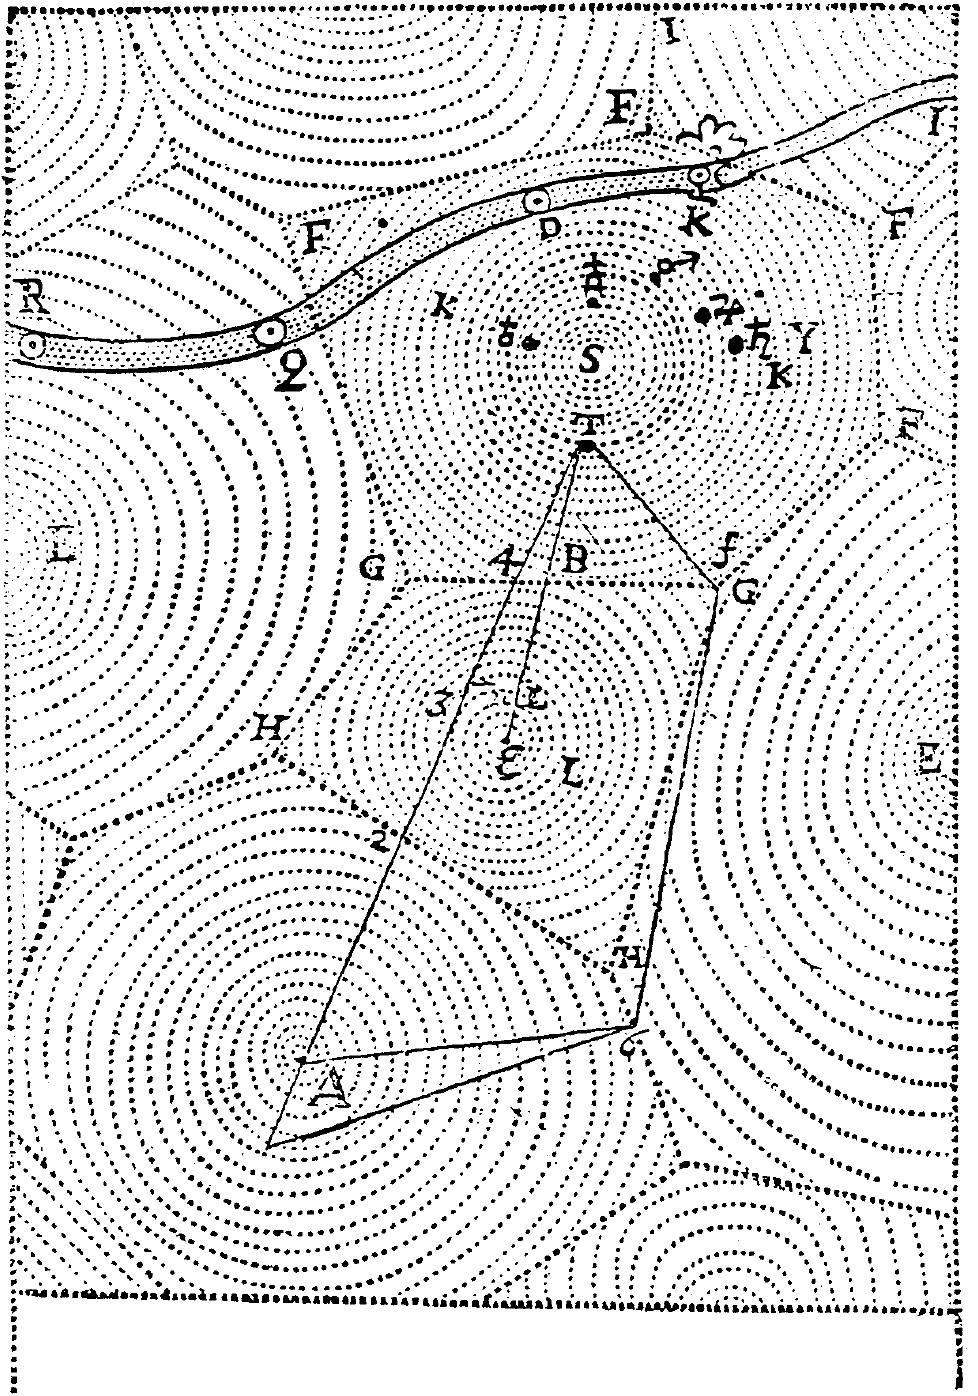
\includegraphics[width=.4\textwidth]{descartes_transparent_heavenly}
      \caption{Descartes' Heavenly Regions}
      \label{fig:descartes_heavenly}
    \end{wrapfigure}
   % ABOVE ^^^ IS THIS NOT A CONTRADICTION? Above descartes says that the higher order elements penetrate the lwoer order ones

   % The center, description of which we have delicately and deliberately escaped, is a star: a heavenly body composed entirely of the first element. The bodies which are composed of the second element and which turn about a center are called the heavens \citep[][p. 35]{descartes}. \par

   Descartes' depicted his cosmological understanding with a diagram, one most directly likened to a Voronoi diagram through his description of the heavens as a whole. Shown in \cref{fig:descartes_heavenly}, there is a heaven (we might call it a heavenly region) for each star. He writes: \say{So there are as many different heavens as there are stars, and since the number of stars is indefinite so too is the number of heavens. And the firmament is just a surface without thickness separating all the heavens from one another,}\citep[p. 35]{descartes}. The heavens, then, is a system of vortices whose centers are these heavenly bodies.\par

   With Descartes' cosmology in the back of our minds, we look to \cref{fig:descartes_heavenly}. What Descartes has drawn around each star are (roughly) concentric circles representing the matter turning about the star. Examining the region near $S$ more closely, we can see that the largest circles intersect with the circles emanating out of the other stars. In Descartes' terms, when circles surrounding a given star intersect with another set of circles, they do so at the \emph{firmament}, which separates the heavenly regions from another. Visually, the firmament between any two heavenly regions--- take, for example, $S$ and $\epsilon$ --- occurs along the set of points equidistant from both $S$ and $\epsilon$. The \say{corners} of the firmament, as Descartes calls them, are points where three circles--- each originating from a distinct heavenly body--- intersect. Many believe Descartes to be the first to depict our own object of study, the Voronoi diagram.\par
   % For those who are already familiar with the Voronoi diagram, it is easy to recognize the visual similarities between Descartes' graphical representation of the heavens and the Voronoi diagram. Perhaps more interesting, however, are the similarities between what he understands the diagram to be and the definition of a Voronoi diagram. As we mentioned earlier, Descartes believes that every star has a heaven associated with it. For example, the matter in the region defined as \textsc{hggh} is the heaven which rotates around $\epsilon$. Similarly, the heaven of star $S$ is precisely the matter in the region \textsc{fggf}. When we define the Voronoi diagram of a set of sites, we will note that every site has a corresponding region. The \emph{firmament}, as Descartes calls it, can be readily adapted to the Voronoi diagram with a shift in jargon: the firmament which separates the heavens from each other are referred to as \emph{edges} in the Voronoi diagram. Should we have the desire to squint, we might even be able to glimpse an oblique reference to a Voronoi vertex: Descartes writes of the matter which lives at the intersection of three or more circles, at what appear to be \say{corners} of the firmament, it is likely smaller, and less agitated than the matter surrounding it.  

  % section the_world (end)

  \section{Definition of the Voronoi Tessellation in $\mathds{R}^d$} % (fold)
  \label{sec:definition_of_the_voronoi_diagram_in_rd}
    Rather than dwelling on Descartes' understanding of the cosmos, we focus on the mathematical diagram that his picture evokes. To that end, let $P:=\{p_{1}, p_{2},\ldots, p_{n}\}$ be a finite set of $n$ distinct points in $\mathds{R}^d$. The Voronoi diagram of $P$, $\mbox{Vor}(P)$, is a division of $\mathds{R}^d$ into $n$ regions. Specifically, $$\mbox{Vor}(P):=\{V_{1}, V_{2}, \ldots, V_{n}\}$$ where each region $V_{i}$ is defined by 
    $$V_{i} := \{\,q \in \mathds{R}^d \mid \delta(q, p_{i}) \leq \delta(q, p_{j}) \text{ for all }\, p_{j}\in P\,\text{ where }j\neq i \}.$$ We take the $\delta(q, p)$ to be $\lVert p-q \rVert$, the usual measure of distance in $\mathds{R}^d$. 
     \Cref{fig:first_sight} shows a Voronoi diagram of nine sites in the plane $\mathds{R}^2$.\par

    \begin{figure}[!htb]
      \centering
      \input{figs/intro/first_sight.tex}
      \caption{A Voronoi Diagram on nine sites}
      \label{fig:first_sight}
    \end{figure} 

    The Voronoi diagram in $\mathds{R}^2$ consists of Voronoi vertices, Voronoi regions, and Voronoi edges. For the purposes of this thesis, we will be working with diagrams in $\mathds{R}^2$. We compute the diagram on a set of sites, $P$, which are points in $\mathds{R}^2$. A Voronoi region, or cell, is bounded by Voronoi edges; every point contained within the region is closer to the site associated with that region than it is to any other site. Voronoi edges, represented by solid lines in \cref{fig:first_sight}, are the set of points which are equidistant from the sites on either side of the edge. These edges intersect at Voronoi vertices; every vertex is equidistant to three sites.\par 

    As we have just seen, the Voronoi diagram is a tiling of the plane $\mathds{R}^2$ according to a proximity relationship between the point-set $P$ and the points in the plane. In the next sections, we pick apart the Voronoi diagram and related structures. In deepening our understanding of the diagram, we will see that the information about proximity that the Voronoi diagram encodes can be applied to an array of problems in both \say{real life} and computational geometry, among many other areas of interest. 

    % section definition_of_the_voronoi_diagram_in_re_d_ (end)
  
  \section{A Half-Plane Characterization} % (fold)
  \label{sec:half_plane_char}
    Every Voronoi region can be thought of as a (possibly unbounded) convex polygon whose edges are the bounding lines of the convex regions and whose vertices are the points of intersection between the bounding lines.  Let's unpack that a little bit. Given two sites $p_{i}$ and $p_{j}$, imagine the line, $\ell$ connecting them. Let $b$ be the perpendicular bisector of $\ell$, which splits the plane into two half-planes. Define the half-plane along $b$ containing $p_{i}$ with $h(p_{i}, p_{j})$; similarly, define the half-plane containing $p_{j}$ with $h(p_{j}, p_{i})$. We can connect this notion of half-planes to our original definition of a Voronoi region: note that with the exception of the set of points lying on $b$, all of the points in $h(p_{i}, p_{j})$ will \emph{not} be in $p_{j}$'s region, since every point in $h(p_{i}, p_{j})$ is closer to $p_{i}$ than it is to $p_{j}$. The points lying along $b$ will be included in both regions, since they are equidistant from $p_{i}$ and $p_{j}$. The dashed line in \cref{fig:one_half_plane} is the perpendicular bisector of $p$ and $q$. The shaded region represents the half-plane $h(p, q)$.\par

    Define set of half-planes containing $p_{i}$ as $H_{i} := \{\,h(p_{i}, p_{j}) \mid j\neq i \}$. There are $n-1$ half-planes in $H_{i}$. Consider the intersection of any two of these half-planes, $h(p_{i}, p_{j})$ and $h(p_{i}, p_{k})$. The set of points lying in the intersection of $h(p_{i}, p_{j})$ and $h(p_{i}, p_{k})$ are all of the points which are at least as close or closer to $p_{i}$ as they are to $p_{j}$ or $p_{k}$. Extrapolating a bit further, if we performed this intersection over all $n-1$ half-planes, we would have the necessary information to determine the set of points which are at least as close or closer to $p_{i}$ as they are to all other sites. Which is, of course, the description of the $V_{i}$ exactly. So we can also describe the region as the intersection of a set of half-planes:

    $$V_{i} = \bigcap_{j \neq i} h(p_{i}, p_{j})$$ 

    \Cref{fig:all_half_planes} illustrates how $V_{p}$ is formed by the intersection of half-planes, it is the darkest shaded region bounded by a solid border.\par

    \begin{figure}[H]
      \centering
      \begin{subtable}{.475\textwidth}
        % Define new PST objects, if not already defined
\ifx\PSTloaded\undefined
\def\PSTloaded{t}
\psset{arrowsize=.01 3.2 1.4 .3}
\psset{dotsize=.2}
\catcode`@=11

\newpsobject{PST@Border}{psline}{linewidth=.003,linestyle=solid}
\newpsobject{PST@Axes}{psline}{linewidth=.0015,linestyle=dotted,dotsep=.004}
\newpsobject{PST@Solid}{psline}{linewidth=.0015,linestyle=solid}
\newpsobject{PST@Dashed}{psline}{linewidth=.0025,linestyle=dashed,dash=.01 .01}
\newpsobject{PST@Dotted}{psline}{linewidth=.0025,linestyle=dotted,dotsep=.008}
\newpsobject{PST@LongDash}{psline}{linewidth=.0015,linestyle=dashed,dash=.02 .01}
\newpsobject{PST@Diamond}{psdots}{linewidth=.001,linestyle=solid,dotstyle=square,dotangle=45}
\newpsobject{PST@Filldiamond}{psdots}{linewidth=.001,linestyle=solid,dotstyle=square*,dotangle=45}
\newpsobject{PST@Cross}{psdots}{linewidth=.001,linestyle=solid,dotstyle=+,dotangle=45}
\newpsobject{PST@Plus}{psdots}{linewidth=.001,linestyle=solid,dotstyle=+}
\newpsobject{PST@Square}{psdots}{linewidth=.001,linestyle=solid,dotstyle=square}
\newpsobject{PST@Circle}{psdots}{linewidth=.001,linestyle=solid,dotstyle=o}
\newpsobject{PST@Triangle}{psdots}{linewidth=.001,linestyle=solid,dotstyle=triangle}
\newpsobject{PST@Pentagon}{psdots}{linewidth=.001,linestyle=solid,dotstyle=pentagon}
\newpsobject{PST@Fillsquare}{psdots}{linewidth=.001,linestyle=solid,dotstyle=square*}
\newpsobject{PST@Fillcircle}{psdots}{linewidth=.001,linestyle=solid,dotstyle=*}
\newpsobject{PST@Filltriangle}{psdots}{linewidth=.001,linestyle=solid,dotstyle=triangle*}
\newpsobject{PST@Fillpentagon}{psdots}{linewidth=.001,linestyle=solid,dotstyle=pentagon*}
\newpsobject{PST@Arrow}{psline}{linewidth=.001,linestyle=solid}
\catcode`@=12

\fi
\psset{unit=\textwidth,xunit=\textwidth,yunit=\textwidth}
\pspicture(0.000000,0.000000)(1.000000,1.000000)
\ifx\nofigs\undefined
\catcode`@=11


% eqn: y = 0.876946-0.305226 x

% \pspolygon[linecolor=white, fillstyle=solid,fillcolor=gray,opacity=0.15](0.0, 0.0)(0.0,0.876946)(1.0, .57172)(1.0,0.0)
% \psline[linestyle=dashed](0.0,0.876946)(1.0, .57172)
% \psline(0.3150,0.7808)
% (0.5427,0.7113)


% y = 0.858998-1.23189 x
\pspolygon[linecolor=white, fillstyle=solid,fillcolor=gray,opacity=0.15](0.0, 1.0)(0.0,0.858998)(0.697301, 0.0)(1.0,0.0)(1.0,1.0)
\psline[linestyle=dashed](0.0,0.858998)(0.697301, 0.0)
% \psline(0.3605,0.4149)
% (0.2031,0.6088)

% y = 1.53709 x+0.296618
% \pspolygon[linecolor=white, fillstyle=solid,fillcolor=gray,opacity=0.15](0.0, 0.296618)(0.457606, 1.0)(1.0,1.0)(1.0,0.0)(0.0,0.0)
% \psline[linestyle=dashed](0.0,0.296618)(0.457606, 1.0)
% \psline(0.3150,0.7808)
% (0.2031,0.6088)

% y = 0.990173 x+0.0579426
% \pspolygon[linecolor=white, fillstyle=solid,fillcolor=gray,opacity=0.15](0.0,0.0579426)(0.0,1.0)(0.951407, 1.0)
% \psline[linestyle=dashed](0.0,0.0579426)(0.951407, 1.0)
% \psline(0.5742,0.6265)
% (0.3605,0.4149)

% %  y = 2.17228-2.69206 x
% \pspolygon[linecolor=white, fillstyle=solid,fillcolor=gray,opacity=0.15](0.0, 0.0)(0.0, 1.0)(0.0,1.0)(0.435458, 1.0)(0.806921,0.0)
% \psline[linestyle=dashed](0.806921,0.0)(0.435458, 1.0)
% \psline(0.5427,0.7113)
% (0.5742,0.6265)

% \psline(0.3565,0.3639)
% (0.3605,0.4149)

% \psline(0.7035,0.5732)
% (0.9519,0.6751)

% \psline(0.7324,0.3287)
% (0.7035,0.5732)

% \psline(0.5742,0.6265)
% (0.7035,0.5732)

% \psline(0.5410,0.2304)
% (0.3565,0.3639)

% \psline(0.5410,0.2304)
% (0.7324,0.3287)

% \psline(0.5427,0.7113)
% (0.6412,0.9678)



% \psline(0.7324,0.3287)
% (0.9509,0.2326)

% \psline(0.5410,0.2304)
% (0.5523,0.0320)

% \psline(0.2031,0.6088)
% (0.0400,0.6170) 

% \psline(0.3150,0.7808)
% (0.2440,0.9679)

% \psline(0.3565,0.3639)
% (0.0583,0.1580)

\psdots[linecolor=gray](0.1426,0.4554)
\psdots[linecolor=gray](0.1587,0.7674)
\psdots(0.3674,0.6343)
% \psdots[linecolor=gray](0.3694,0.1336)
\psdots[linecolor=gray](0.4416,0.8727)
\psdots[linecolor=gray](0.5821,0.4217)
% \psdots[linecolor=gray](0.7225,0.1534)
\psdots[linecolor=gray](0.7265,0.7654)
% \psdots[linecolor=gray](0.8570,0.4534)

\rput[l](0.4,0.6343){$p$}
\rput[r](0.12,0.4554){$q$}

\rput[b]{-45}(0.55,0.2){$h(p, q)$}

% \PST@Circle(0.3150,0.7808)
% \PST@Circle(0.5427,0.7113)
% \PST@Circle(0.2031,0.6088)
% \PST@Circle(0.5742,0.6265)
% \PST@Circle(0.7035,0.5732)
% \PST@Circle(0.3605,0.4149)
% \PST@Circle(0.7324,0.3287)
% \PST@Circle(0.3565,0.3639)
% \PST@Circle(0.5410,0.2304)
\catcode`@=12
\fi
\endpspicture

        \caption{One half-plane, $h(p, q)$}
        \label{fig:one_half_plane}
      \end{subtable}%
      \begin{subtable}{.475\textwidth}
      \centering
        \input{figs/intro/half_plane.tex}
        \caption{$V_{p}$ from half-plane intersections}
        \label{fig:all_half_planes}
      \end{subtable}
      \caption{Half-Plane Intersections}
      \label{fig:half_planes}
    \end{figure}

    Recall that a set is convex if the line segment connecting any two points in the set is also in the region. Because the half-plane is a convex set and the intersection of convex regions is also convex, the Voronoi region is convex. In \cref{sec:a_naive_approach} we describe an algorithm to construct the Voronoi diagram using an approach which relies on half-plane intersections.\par

    % In summary, every Voronoi region can be thought of as a (possibly unbounded) convex polygon whose edges are the bounding lines of the convex regions and whose vertices are the points of intersection between the bounding lines. 

    Note that some of the edges will be line segments, while others will extend out towards infinity. We will refer to the latter type of edge as a \emph{half infinite edge}. Since each Voronoi region was the result of $n-1$ half-plane intersections, we know that each such region has, at most, $n-1$ edges. \par
  % section  (end)

  \section{The Dual} % (fold)
  \label{sec:the_dual}
    While the Voronoi diagram can be computed directly with relative--- though certainly not always computational--- ease, it can also be computed somewhat indirectly, that is, through the construction of its dual, the \emph{Delaunay subdivision}. For those not already familiar with the idea of duality, choose a site $p_{i} \in P$. Using $\mbox{Vor}(P)$ as a reference, draw a line connecting $p_{i}$ to the sites of the regions adjacent to it, as in \cref{fig:del_intuition1}. Do this for all the sites. The resulting diagram is the unique Delaunay triangulation of $P$, shown in \cref{fig:del_intuition2}.\par

    If we assume that the set of sites $P$ is \say{well-behaved,}\footnote{We'll wave our hands at this for now, and in \cref{sec:the_fine_print} we'll define more precisely what it means for the set of sites to be \say{well-behaved.}} then the resulting diagram is the unique Delaunay triangulation of those sites, $\mbox{Del}(P)$. In particular, we'll assume that exactly three Voronoi regions meet at every Voronoi vertex for the remainder of this discussion. One of the many advantages of working with this dual is the ability to work with triangular faces instead of with polygonal regions with an unknown number of sides. \par

    % We can develop our intuition for the Delaunay triangulation and the primal-dual relationship by constructing $\mbox{Del}(P)$ from $\mbox{Vor}(P)$. 

    To get an idea for this entity before its definition, choose a site $p_{i} \in P$. Using $\mbox{Vor}(P)$ as a reference, draw a line connecting $p_{i}$ to the sites of the regions adjacent to it, as in \cref{fig:del_intuition1}. Do this for all the sites. The resulting diagram is the unique Delaunay Triangulation of $P$, as shown in \cref{fig:del_intuition2}.

    \begin{figure}[!htb]
      \centering
      \begin{subtable}{.475\textwidth}
        % Define new PST objects, if not already defined
\ifx\PSTloaded\undefined
\def\PSTloaded{t}
\psset{arrowsize=.01 3.2 1.4 .3}
\psset{dotsize=.2}
\catcode`@=11

\newpsobject{PST@Border}{psline}{linewidth=.003,linestyle=solid}
\newpsobject{PST@Axes}{psline}{linewidth=.0015,linestyle=dotted,dotsep=.004}
\newpsobject{PST@Solid}{psline}{linewidth=.0015,linestyle=solid}
\newpsobject{PST@Dashed}{psline}{linewidth=.0025,linestyle=dashed,dash=.01 .01}
\newpsobject{PST@Dotted}{psline}{linewidth=.0025,linestyle=dotted,dotsep=.008}
\newpsobject{PST@LongDash}{psline}{linewidth=.0015,linestyle=dashed,dash=.02 .01}
\newpsobject{PST@Diamond}{psdots}{linewidth=.001,linestyle=solid,dotstyle=square,dotangle=45}
\newpsobject{PST@Filldiamond}{psdots}{linewidth=.001,linestyle=solid,dotstyle=square*,dotangle=45}
\newpsobject{PST@Cross}{psdots}{linewidth=.001,linestyle=solid,dotstyle=+,dotangle=45}
\newpsobject{PST@Plus}{psdots}{linewidth=.001,linestyle=solid,dotstyle=+}
\newpsobject{PST@Square}{psdots}{linewidth=.001,linestyle=solid,dotstyle=square}
\newpsobject{PST@Circle}{psdots}{linewidth=.001,linestyle=solid,dotstyle=o}
\newpsobject{PST@Triangle}{psdots}{linewidth=.001,linestyle=solid,dotstyle=triangle}
\newpsobject{PST@Pentagon}{psdots}{linewidth=.001,linestyle=solid,dotstyle=pentagon}
\newpsobject{PST@Fillsquare}{psdots}{linewidth=.001,linestyle=solid,dotstyle=square*}
\newpsobject{PST@Fillcircle}{psdots}{linewidth=.001,linestyle=solid,dotstyle=*}
\newpsobject{PST@Filltriangle}{psdots}{linewidth=.001,linestyle=solid,dotstyle=triangle*}
\newpsobject{PST@Fillpentagon}{psdots}{linewidth=.001,linestyle=solid,dotstyle=pentagon*}
\newpsobject{PST@Arrow}{psline}{linewidth=.001,linestyle=solid}
\catcode`@=12

\fi
\psset{unit=\textwidth,xunit=\textwidth,yunit=\textwidth}
\pspicture(0.000000,0.000000)(1.000000,1.000000)
\ifx\nofigs\undefined
\catcode`@=11

\PST@Border(0.3150,0.7808)
(0.3150,0.7808)
(0.5427,0.7113)

\PST@Border(0.2031,0.6088)
(0.2031,0.6088)
(0.3605,0.4149)

\PST@Border(0.7035,0.5732)
(0.7035,0.5732)
(0.9519,0.6751)

\PST@Border(0.7324,0.3287)
(0.7324,0.3287)
(0.7035,0.5732)

\PST@Border(0.5742,0.6265)
(0.5742,0.6265)
(0.7035,0.5732)

\PST@Border(0.5410,0.2304)
(0.5410,0.2304)
(0.3565,0.3639)

\PST@Border(0.3565,0.3639)
(0.3565,0.3639)
(0.3605,0.4149)

\PST@Border(0.5427,0.7113)
(0.5427,0.7113)
(0.3150,0.7808)

\PST@Border(0.2031,0.6088)
(0.2031,0.6088)
(0.0400,0.6170)

\PST@Border(0.5410,0.2304)
(0.5410,0.2304)
(0.7324,0.3287)

\PST@Border(0.3565,0.3639)
(0.3565,0.3639)
(0.5410,0.2304)

\PST@Border(0.3605,0.4149)
(0.3605,0.4149)
(0.3565,0.3639)

\PST@Border(0.5427,0.7113)
(0.5427,0.7113)
(0.6412,0.9678)

\PST@Border(0.7324,0.3287)
(0.7324,0.3287)
(0.9509,0.2326)

\PST@Border(0.3605,0.4149)
(0.3605,0.4149)
(0.2031,0.6088)

\PST@Border(0.7324,0.3287)
(0.7324,0.3287)
(0.9509,0.2326)

\PST@Border(0.5410,0.2304)
(0.5410,0.2304)
(0.5523,0.0320)

\PST@Border(0.7035,0.5732)
(0.7035,0.5732)
(0.7324,0.3287)

\PST@Border(0.5742,0.6265)
(0.5742,0.6265)
(0.5427,0.7113)

\PST@Border(0.7324,0.3287)
(0.7324,0.3287)
(0.5410,0.2304)

\PST@Border(0.3150,0.7808)
(0.3150,0.7808)
(0.2440,0.9679)

\PST@Border(0.5410,0.2304)
(0.5410,0.2304)
(0.5523,0.0320)

\PST@Border(0.2031,0.6088)
(0.2031,0.6088)
(0.0400,0.6170)

\PST@Border(0.2031,0.6088)
(0.2031,0.6088)
(0.3150,0.7808)

\PST@Border(0.5427,0.7113)
(0.5427,0.7113)
(0.6412,0.9678)

\PST@Border(0.3150,0.7808)
(0.3150,0.7808)
(0.2031,0.6088)

\PST@Border(0.7035,0.5732)
(0.7035,0.5732)
(0.5742,0.6265)

\PST@Border(0.5742,0.6265)
(0.5742,0.6265)
(0.3605,0.4149)

\PST@Border(0.3605,0.4149)
(0.3605,0.4149)
(0.5742,0.6265)

\PST@Border(0.5427,0.7113)
(0.5427,0.7113)
(0.5742,0.6265)

\PST@Border(0.3150,0.7808)
(0.3150,0.7808)
(0.2440,0.9679)

\PST@Border(0.3565,0.3639)
(0.3565,0.3639)
(0.0583,0.1580)

\PST@Border(0.7035,0.5732)
(0.7035,0.5732)
(0.9519,0.6751)

\PST@Border(0.3565,0.3639)
(0.3565,0.3639)
(0.0583,0.1580)

\PST@Dashed(0.1426,0.4554)
(0.1426,0.4554)
(0.3694,0.1336)

\PST@Dashed(0.1426,0.4554)
(0.1426,0.4554)
(0.5821,0.4217)

\PST@Dashed(0.1426,0.4554)
(0.1426,0.4554)
(0.1587,0.7674)

\PST@Dashed(0.1587,0.7674)
(0.1587,0.7674)
(0.1426,0.4554)

\PST@Dashed(0.3674,0.6343)
(0.3674,0.6343)
(0.1426,0.4554)

\PST@Dashed(0.5821,0.4217)
(0.5821,0.4217)
(0.1426,0.4554)

\PST@Dashed(0.1426,0.4554)
(0.1426,0.4554)
(0.3674,0.6343)

\PST@Dashed(0.3694,0.1336)
(0.3694,0.1336)
(0.1426,0.4554)

\PST@Fillcircle(0.1426,0.4554)
\PST@Fillcircle(0.1587,0.7674)
\PST@Fillcircle(0.4416,0.8727)
\PST@Fillcircle(0.7265,0.7654)
\PST@Fillcircle(0.8570,0.4534)
\PST@Fillcircle(0.7225,0.1534)
\PST@Fillcircle(0.3694,0.1336)
\PST@Fillcircle(0.3674,0.6343)
\PST@Fillcircle(0.5821,0.4217)
\PST@Circle(0.3150,0.7808)
\PST@Circle(0.5427,0.7113)
\PST@Circle(0.2031,0.6088)
\PST@Circle(0.5742,0.6265)
\PST@Circle(0.7035,0.5732)
\PST@Circle(0.3605,0.4149)
\PST@Circle(0.7324,0.3287)
\PST@Circle(0.3565,0.3639)
\PST@Circle(0.5410,0.2304)
\catcode`@=12
\fi
\endpspicture

        \caption{A site connected to its adjacent sites}
        \label{fig:del_intuition1}
      \end{subtable}%
      \begin{subtable}{.475\textwidth}
        \input{figs/intro/del_intuition_done.tex}
        \caption{All sites connected to neighboring sites}
        \label{fig:del_intuition2}
      \end{subtable}
      \caption{Voronoi Diagram (Solid) and Delaunay Triangulation (Dashed)}
      \label{fig:del_intuition}
    \end{figure}

    % move degenerate case to a last paragraph where you can finally be honest with them
    % Note that we are being a bit cavalier with this description of the Delaunay triangulation. If four or more sites were co-circular, our result would be a Delaunay subdivision, which could be quickly modified (via the addition of edges, if necessary) to be a Delaunay triangulation. Furthermore, the Delaunay triangulation of a  Voronoi diagram whose sites are in general position is unique.\par

    Let's take a couple steps back and work to define the Delaunay triangulation a bit more rigorously, so we can better examine its properties and relation to the Voronoi diagram. It's useful, for our purposes, to consider the \emph{convex hull}. The convex hull of a set of points $P$ is the smallest convex region containing $P$. Roughly, it is the intersection of all of the convex sets containing $P$. Precisely: given points $q_{1}$,... $q_{k}$, a \emph{convex combination} of those points is defined as $\Sigma\alpha_{i}q_{i}$, where the $\alpha_{i}$'s are non-negative and $\Sigma\alpha_{i}=1.$  So, for our point set $P$, we are interested in the convex hull, denoted $\mbox{conv}(P)$, defined as the set:

    $$
     \mbox{conv}(P) = \{\, \alpha_{1}p_{1} + ... + \alpha_{n}p_{n} \ \mid\ \text{for$ \,\alpha_{i} \in \Re, \; \alpha_{i} \geq 0$ and $\Sigma\alpha_{i} = 1$}\,\} 
    $$

    \Cref{fig:convex_hull} illustrates the convex hull of the same point set used in \cref{fig:del_intuition1,fig:del_intuition2}. 
    This region of the plane is best understood in terms of a complete description of its boundary, as shown in \cref{fig:convex_hull}.\par

    \begin{figure}[!htb]
      \centering
      
% Define new PST objects, if not already defined
\ifx\PSTloaded\undefined
\def\PSTloaded{t}
\psset{arrowsize=.01 3.2 1.4 .3}
\psset{dotsize=.2}
\catcode`@=11

\newpsobject{PST@Border}{psline}{linewidth=.003,linestyle=solid}
\newpsobject{PST@Axes}{psline}{linewidth=.0015,linestyle=dotted,dotsep=.004}
\newpsobject{PST@Solid}{psline}{linewidth=.0015,linestyle=solid}
\newpsobject{PST@Dashed}{psline}{linewidth=.0015,linestyle=dashed,dash=.01 .01}
\newpsobject{PST@Dotted}{psline}{linewidth=.0025,linestyle=dotted,dotsep=.008}
\newpsobject{PST@LongDash}{psline}{linewidth=.0015,linestyle=dashed,dash=.02 .01}
\newpsobject{PST@Diamond}{psdots}{linewidth=.001,linestyle=solid,dotstyle=square,dotangle=45}
\newpsobject{PST@Filldiamond}{psdots}{linewidth=.001,linestyle=solid,dotstyle=square*,dotangle=45}
\newpsobject{PST@Cross}{psdots}{linewidth=.001,linestyle=solid,dotstyle=+,dotangle=45}
\newpsobject{PST@Plus}{psdots}{linewidth=.001,linestyle=solid,dotstyle=+}
\newpsobject{PST@Square}{psdots}{linewidth=.001,linestyle=solid,dotstyle=square}
\newpsobject{PST@Circle}{psdots}{linewidth=.001,linestyle=solid,dotstyle=o}
\newpsobject{PST@Triangle}{psdots}{linewidth=.001,linestyle=solid,dotstyle=triangle}
\newpsobject{PST@Pentagon}{psdots}{linewidth=.001,linestyle=solid,dotstyle=pentagon}
\newpsobject{PST@Fillsquare}{psdots}{linewidth=.001,linestyle=solid,dotstyle=square*}
\newpsobject{PST@Fillcircle}{psdots}{linewidth=.001,linestyle=solid,dotstyle=*}
\newpsobject{PST@Filltriangle}{psdots}{linewidth=.001,linestyle=solid,dotstyle=triangle*}
\newpsobject{PST@Fillpentagon}{psdots}{linewidth=.001,linestyle=solid,dotstyle=pentagon*}
\newpsobject{PST@Arrow}{psline}{linewidth=.001,linestyle=solid}
\catcode`@=12

\fi
\psset{unit=2.5in,xunit=2.5in,yunit=2.5in}
\pspicture(0.000000,0.000000)(1.000000,1.000000)
\ifx\nofigs\undefined
\catcode`@=11

% .1426
% .1587
% .3694

\PST@Border(0.1426,0.4554)
(0.1426,0.4554)
(0.3694,0.1336)

% \PST@Border(0.7265,0.7654)
% (0.7265,0.7654)
% (0.8570,0.4534)

% \PST@Border(0.1587,0.7674)
% (0.1587,0.7674)
% (0.3674,0.6343)

% \PST@Border(0.1426,0.4554)
% (0.1426,0.4554)
% (0.5821,0.4217)

\PST@Border(0.3694,0.1336)
(0.3694,0.1336)
(0.7225,0.1534)

% \PST@Border(0.5821,0.4217)
% (0.5821,0.4217)
% (0.3694,0.1336)

\PST@Border(0.7225,0.1534)
(0.7225,0.1534)
(0.3694,0.1336)

\PST@Border(0.1426,0.4554)
(0.1426,0.4554)
(0.1587,0.7674)

\PST@Border(0.1587,0.7674)
(0.1587,0.7674)
(0.4416,0.8727)

% \PST@Border(0.5821,0.4217)
% (0.5821,0.4217)
% (0.8570,0.4534)

% \PST@Border(0.8570,0.4534)
% (0.8570,0.4534)
% (0.5821,0.4217)

% \PST@Border(0.5821,0.4217)
% (0.5821,0.4217)
% (0.3674,0.6343)

\PST@Border(0.1587,0.7674)
(0.1587,0.7674)
(0.1426,0.4554)

% \PST@Border(0.7225,0.1534)
% (0.7225,0.1534)
% (0.5821,0.4217)

% \PST@Border(0.3674,0.6343)
% (0.3674,0.6343)
% (0.1426,0.4554)

% \PST@Border(0.5821,0.4217)
% (0.5821,0.4217)
% (0.7265,0.7654)

% \PST@Border(0.3674,0.6343)
% (0.3674,0.6343)
% (0.4416,0.8727)

% \PST@Border(0.7265,0.7654)
% (0.7265,0.7654)
% (0.5821,0.4217)

% \PST@Border(0.3674,0.6343)
% (0.3674,0.6343)
% (0.5821,0.4217)

% \PST@Border(0.4416,0.8727)
% (0.4416,0.8727)
% (0.3674,0.6343)

\PST@Border(0.4416,0.8727)
(0.4416,0.8727)
(0.1587,0.7674)

\PST@Border(0.7225,0.1534)
(0.7225,0.1534)
(0.8570,0.4534)

\PST@Border(0.7265,0.7654)
(0.7265,0.7654)
(0.4416,0.8727)

% \PST@Border(0.3694,0.1336)
% (0.3694,0.1336)
% (0.5821,0.4217)

% \PST@Border(0.5821,0.4217)
% (0.5821,0.4217)
% (0.1426,0.4554)

% \PST@Border(0.1426,0.4554)
% (0.1426,0.4554)
% (0.3674,0.6343)

% \PST@Border(0.5821,0.4217)
% (0.5821,0.4217)
% (0.7225,0.1534)

\PST@Border(0.8570,0.4534)
(0.8570,0.4534)
(0.7225,0.1534)

% \PST@Border(0.3674,0.6343)
% (0.3674,0.6343)
% (0.1587,0.7674)

\PST@Border(0.4416,0.8727)
(0.4416,0.8727)
(0.7265,0.7654)

\PST@Border(0.8570,0.4534)
(0.8570,0.4534)
(0.7265,0.7654)

% \PST@Border(0.7265,0.7654)
% (0.7265,0.7654)
% (0.3674,0.6343)

\PST@Border(0.3694,0.1336)
(0.3694,0.1336)
(0.1426,0.4554)

% \PST@Border(0.3674,0.6343)
% (0.3674,0.6343)
% (0.7265,0.7654)

\PST@Fillcircle(0.1426,0.4554)
\PST@Fillcircle(0.1587,0.7674)
\PST@Fillcircle(0.4416,0.8727)
\PST@Fillcircle(0.7265,0.7654)
\PST@Fillcircle(0.8570,0.4534)
\PST@Fillcircle(0.7225,0.1534)
\PST@Fillcircle(0.3694,0.1336)
\PST@Fillcircle(0.3674,0.6343)
\PST@Fillcircle(0.5821,0.4217)

\catcode`@=12
\fi
\endpspicture

      \caption{Convex hull of a set of points}
      \label{fig:convex_hull}
    \end{figure}

    A triangulation is a subdivision of the plane into triangular faces. More specifically, the triangulation of a point-set is a set of non-overlapping triangles where the union of the regions bounded by the triangles is the convex hull of $P$. The vertices of the triangles are taken from the point set, and each point in the set must be the vertex of at least one triangle. The boundary of the Delaunay triangulation of P is the convex hull of $P$. It's important to note here that every edge in the convex hull of a set of sites is an edge in the Delaunay triangulation.\par

    We can confirm the Delaunayhood of a triangulation in two ways. For two sites $a, b \in P$, we say that that the edge $\overline{ab}$ connecting them is Delaunay if and only if there is a circle passing through them that contains no other sites in $P$. When this is true, we call the edge \emph{locally Delaunay}. When every edge in the triangulation is locally Delaunay, we may say that the triangulation is \emph{globally Delaunay}. An equivalent understanding of the Delaunay property operates on the faces of the triangulation instead of its edges. It is often referred to as the \emph{empty circle condition}. The \emph{empty circle condition} stipulates that for a triangle defined by three sites $a, b, c \in P$, the circumcircle of that triangle contains no other sites in $P$. These tests correspond to the geometric properties of the corresponding Voronoi diagram. Asking whether or not a face of the triangulation satisfies the empty circle condition is equivalent to checking whether or not a circle centered at a Voronoi vertex includes no sites and intersects with three sites.\par

    So, given a triangulation, as in \cref{fig:delaunayhood_small}, one way to confirm its Delaunayhood is as follows: for each edge $e$ in the triangulation, we consider the two triangles on either side of the edge.  In the case of \cref{fig:delaunayhood_small}, the triangles which share edge $e$ are $\Delta dab$ and $\Delta bcd$. Because $a$ is not contained in the circumcircle of $\Delta bcd$, shown as a dashed line in \cref{fig:delaunayhood_small}, we say that $e$ passes the circle test. Specifically, we have shown that there is a circle namely, the circle passing through $b$, $c$, and $d$, that does not contain $a$ or $c$. Symmetrically, we could ask whether or not $c$ is contained in the circumcircle of $\Delta dab$, another possible circle.\par

    \begin{figure}[!htb]
      \centering
      
% Define new PST objects, if not already defined
\ifx\PSTloaded\undefined
\def\PSTloaded{t}
% \psset{arrowsize=.01 3.2 1.4 .3}
\psset{dotsize=.2}
\catcode`@=11
\catcode`@=12

\fi
% \psset{unit=2in,xunit=2in,yunit=2in}
\psset{unit=.33\textwidth,xunit=.33\textwidth,yunit=.33\textwidth}
\pspicture(-0.25000, 0.000)(.7500,.8)
\ifx\nofigs\undefined
\catcode`@=11

%labels
\rput[b](.25, .80){$a$}
\rput[Br](-0.05, 0.25){$b$}
\rput[t](.35, .075){$c$}
\rput[Bl](.55, .5){$d$}

\rput[b]{30}(.3, .33){$e$}

%sites
\psdots(0.0, 0.25)
\psdots(.5, .5)
\psdots(.25, .75)
\psdots(.375, .125)

%convex hull
\psline(0.0, 0.25)(.25, 0.75)
\psline(.25, 0.75)(.5, .5)
\psline(.5, .5)(.375, .125)
\psline(0.0, 0.25)(.375, .125)

%cross edges
\psline(0.0, 0.25)(.5, .5)

%circle
\pscircle[linestyle=dashed](0.25, 0.375){0.279508}

\catcode`@=12
\fi
\endpspicture

      \caption{Testing the Delaunayhood of a small triangulation}
      \label{fig:delaunayhood_small}
    \end{figure}

    Note that this formulation only confirms the existence of a circle passing through $b$ and $d$ that contains neither $a$ nor $c$. It tell us nothing of the remaining sites in $P$. However, an important result was proven in \textcite{lee}: a triangulation T of the point set $P$ is Delaunay if and only if every edge passes the circle test.

  \section{The Fine Print}
  \label{sec:the_fine_print}
    In the previous section, we waved our hands at the constraint that the set of sites, $P$, be \say{well behaved.} Here, we pause to introduce the notion of \emph{general position}, and to make note of a special case. Later, when we examine more sophisticated algorithms to compute the Voronoi Diagram and Delaunay Triangulation, we will assume that the set of sites is in general position and that the special case is not the case.
    \subsection{General Position} % (fold)
    \label{sub:general_position}
    
      When the set of sites we'd like to operate on is in \emph{general position}, we can rest assured that we will not be tasked with handling any degenerate cases. These degenerate cases result from the geometric constraints which characterize the Delaunay and Voronoi diagrams. We might also note that since it is the enforcement of these properties which causes these special cases, that the notion of general position is particular to the metric we use.\par

      When constructing Delaunay or Voronoi diagrams in Euclidean space we say that a set of sites, $P$, is in \emph{general position} when no four sites in $P$ are co-circular.

      Though it isn't a particularly daunting task to understand why four co-circular sites would result in a degenerate case, it's not an exercise I'll leave to you, dear Reader. It is easiest to see the effects of such a scenario play out in the Delaunay triangulation, but I'll also note how it affects the Voronoi diagram. \par

      Four co-circular sites in $P$ results in a degenerate case because the Delaunay triangulation of $P$ will not be unique. In particular, consider the simplest case of this, as illustrated in \cref{fig:co_circular}. When we attempt to triangulate $abcd$, we have a choice between inserting an edge $bd$ and an edge $ac$. Since both of these edges satisfy the Delaunay condition, we have two valid triangulations of $P$. If we didn't try to triangulate $abcd$ at all, then our Delaunay triangulation would be a Delaunay subdivision, since one of its facets has four sides. The corresponding effect in the Voronoi diagram would be a Voronoi vertex with out-degree four instead of three. 

      \begin{figure}[H]
        \centering
        
% Define new PST objects, if not already defined
\ifx\PSTloaded\undefined
\def\PSTloaded{t}
% \psset{arrowsize=.01 3.2 1.4 .3}
\psset{dotsize=.2}
\catcode`@=11
\catcode`@=12

\fi
% \psset{unit=2in,xunit=2in,yunit=2in}
\psset{unit=.33\textwidth,xunit=.33\textwidth,yunit=.33\textwidth}
\pspicture(-0.25000, -0.12500)(.7500,1.000000)
\ifx\nofigs\undefined
\catcode`@=11

%labels
\rput[b](.25, .80){$a$}
\rput[Br](-0.05, 0.25){$b$}
\rput[Br](-.1, .5){$c$}
\rput[Bl](.55, .3){$d$}

%sites
\psdots(0.0, 0.25) %b
\psdots(.5, .25) %d
\psdots(.25, .75) %a
\psdots(-.051863, .5) %c

%convex hull
\psline(0.0, 0.25)(.5, .25)
\psline(.25, 0.75)(.5, .25)
\psline(.25, .75)(-.051863, .5)
\psline(0.0, 0.25)(-.051863, .5)

%cross edges
% \psline(0.0, 0.25)(.5, .5)

%circle
\pscircle[linestyle=dashed](0.25, 0.4375){0.3125}

\catcode`@=12
\fi
\endpspicture

        \caption{Four Co-circular sites}
        \label{fig:co_circular}
      \end{figure}

      As we will discover in \cref{sec:fortune_s_algorithm}, a Voronoi vertex exists at the center of the circumcircle of the corresponding facet of the Delaunay triangulation. In \cref{fig:co_circular} for example, suppose we inserted edge $ab$. Then we would have two faces, namely $acb$ and $bda$. Since these four sites are co-circular, the circumcircle of the two faces is the same, leading us to insert two Voronoi vertices in the same location (that is to say, the at the center of the circle). Note that we would have had inserted the Voronoi vertex at the same location even if we had inserted edge $bd$. In practice, we will often ignore this degeneracy by allowing two Voronoi vertices in the same location.\par

    % subsection general_position (end)
    \subsection{The Special Case} % (fold)
    \label{sub:special_case}

      When all of the sites in $P$ are collinear, we find ourselves with a special case. Consider one of the simplest scenarios, where $P$ is a set of three collinear sites: $a$, $b$, and $c$, as shown in \cref{fig:collinear}. This time, we'll focus on what the effects would be like in the Voronoi Diagram. The dashed lines in the figure denote the perpendicular bisectors of the line segments connecting adjacent sites.
      \begin{figure}[!htb]
        \centering
        
% Define new PST objects, if not already defined
\ifx\PSTloaded\undefined
\def\PSTloaded{t}
% \psset{arrowsize=.01 3.2 1.4 .3}
\psset{dotsize=.2}
\catcode`@=11
\catcode`@=12

\fi
% \psset{unit=2in,xunit=2in,yunit=2in}
\psset{unit=.33\textwidth,xunit=.33\textwidth,yunit=.33\textwidth}
\pspicture(0.000, -0.2500)(1.000, .75)
\ifx\nofigs\undefined
\catcode`@=11

%labels
\rput[Br](0.20, 0.0){$a$} %b
\rput[Bb](.5, 0.05){$b$} %d
\rput[Bl](.8, 0.0){$c$} %a

%sites
\psdots(0.25, 0.0) %b
\psdots(.5, 0.0) %d
\psdots(.75, 0.0) %a


%lines
\psline[linestyle=dashed, arrowsize=3pt 4]{<->}(0.375, -0.2)(0.375, .70)
\psline[linestyle=dashed, arrowsize=3pt 4]{<->}(0.625, -0.2)(0.625, .70)
\psline[linewidth=1pt, linestyle=dotted](.25, 0.0)(.75, 0.0)
% \psline[linestyle=dashed](0.75, -0.2)(0.75, .5)

%cross edges
% \psline(0.0, 0.25)(.5, .5)

%circle
% \pscircle[linestyle=dashed](0.25, 0.4375){0.3125}

\catcode`@=12
\fi
\endpspicture

        \caption{Voronoi Diagram of Three Collinear Sites}
        \label{fig:collinear}
      \end{figure}

      \noindent More generally, note that if all $n$ sites in $P$ are collinear, then there cannot be a triangulation of these sites. Further, the Voronoi Diagram of $P$ is a set of regions whose boundaries are the $n-1$ parallel lines bisecting adjacent sites. 

    % subsection special_cases (end)


    % In \cref{sec:properties_of_voronoi_and_delaunay_diagrams} we will explore some of the convenient and interesting geometric consequences of a triangulation with the Delaunay property.\par

  \section{A Graph Representation} % (fold)
  \label{sec:a_graph_rep}

    When the dimension of the space in which we compute the Voronoi Diagram or Delaunay triangulation is low (i.e $d = 2,\; d=3 $), it is difficult to divorce the geometric realities of the diagram as it is represented in $\mathds{R}^d$ from the more subtle topological and combinatorial aspects of the diagrams. As the dimension increases, our ability to reason about and visualize the Voronoi diagram and Delaunay Triangulations by relying on its geometric properties diminishes. In this section, we introduce the notion of the Voronoi and, implicitly, Delaunay \emph{graphs}--- where $d=2$--- and shift our focus onto the relationships between the disparate components of the diagrams.\par

    \subsection{Obtaining the Voronoi Graph} % (fold)
    \label{sub:voronoi_graph}

      The various components of a Voronoi diagram--- its edges, vertices, and regions--- relate to each other in a non-geometric way. Namely, there is an underlying combinatorial structure associated with a diagram. Consider the set of edges of a Voronoi diagram. An edge connects two Voronoi vertices. We can leverage this fact to describe the Voronoi diagram in a combinatorial way: as a graph.\par

      Recall that a graph is a collection of vertices and edges. Given $\mbox{Vor}(P)$, let $C$ be the set of Voronoi vertices and let $E$ be the set of Voronoi edges. Every Voronoi edge $e$ in $E$ is a pair $(c_{i}, c_{j})$ for two distinct $c_{i}, c_{j}$  in $C$. Through describing $\mbox{Vor}(P)$ in this way, we recognize it as a graph whose embedding in $\mathds{R}^2$ satisfies the geometric characteristics of the Voronoi diagram.\par

      Our attempts to consider $\mbox{Vor}(P)$ as a graph will be thwarted if we don't address the edges which do not necessarily connect two Voronoi vertices. These are the \emph{half-infinite edges}, discussed in \cref{sec:half_plane_char}. To account for this, we can introduce a vertex \say{at infinity}. Then, we assign the vertex at infinity to be second endpoint of each half infinite edge in the diagram. \Cref{fig:vertex_at_infinity} illustrates how the addition of a vertex at infinity changes the Voronoi diagram of nine sites we saw in \cref{fig:first_sight}.\par

      \begin{figure}[!htb]
        \centering
        % Define new PST objects, if not already defined
\ifx\PSTloaded\undefined
\def\PSTloaded{t}
\psset{arrowsize=.01 3.2 1.4 .3}
\psset{dotsize=.2}
\catcode`@=11

\newpsobject{PST@Border}{psline}{linewidth=.003,linestyle=solid}
\newpsobject{PST@Axes}{psline}{linewidth=.0015,linestyle=dotted,dotsep=.004}
\newpsobject{PST@Solid}{psline}{linewidth=.0015,linestyle=solid}
\newpsobject{PST@Dashed}{psline}{linewidth=.0025,linestyle=dashed,dash=.01 .01}
\newpsobject{PST@Dotted}{psline}{linewidth=.0025,linestyle=dotted,dotsep=.008}
\newpsobject{PST@LongDash}{psline}{linewidth=.0015,linestyle=dashed,dash=.02 .01}
\newpsobject{PST@Diamond}{psdots}{linewidth=.001,linestyle=solid,dotstyle=square,dotangle=45}
\newpsobject{PST@Filldiamond}{psdots}{linewidth=.001,linestyle=solid,dotstyle=square*,dotangle=45}
\newpsobject{PST@Cross}{psdots}{linewidth=.001,linestyle=solid,dotstyle=+,dotangle=45}
\newpsobject{PST@Plus}{psdots}{linewidth=.001,linestyle=solid,dotstyle=+}
\newpsobject{PST@Square}{psdots}{linewidth=.001,linestyle=solid,dotstyle=square}
\newpsobject{PST@Circle}{psdots}{linewidth=.001,linestyle=solid,dotstyle=o}
\newpsobject{PST@Triangle}{psdots}{linewidth=.001,linestyle=solid,dotstyle=triangle}
\newpsobject{PST@Pentagon}{psdots}{linewidth=.001,linestyle=solid,dotstyle=pentagon}
\newpsobject{PST@Fillsquare}{psdots}{linewidth=.001,linestyle=solid,dotstyle=square*}
\newpsobject{PST@Fillcircle}{psdots}{linewidth=.001,linestyle=solid,dotstyle=*}
\newpsobject{PST@Filltriangle}{psdots}{linewidth=.001,linestyle=solid,dotstyle=triangle*}
\newpsobject{PST@Fillpentagon}{psdots}{linewidth=.001,linestyle=solid,dotstyle=pentagon*}
\newpsobject{PST@Arrow}{psline}{linewidth=.001,linestyle=solid}
\catcode`@=12

\fi
\psset{unit=.3\textwidth,xunit=.3\textwidth,yunit=.3\textwidth}
\pspicture(-.25000,-0.25000)(1.250,1.2500)
\ifx\nofigs\undefined
\catcode`@=11

\psline(0.3150,0.7808)(0.5427,0.7113)
\psline(0.7324,0.3287)(0.7035,0.5732)
\psline(0.5742,0.6265)(0.7035,0.5732)
\psline(0.5410,0.2304)(0.3565,0.3639)
\psline(0.5410,0.2304)(0.7324,0.3287)
\psline(0.3605,0.4149)(0.3565,0.3639)
\psline(0.3605,0.4149)(0.2031,0.6088)
\psline(0.2031,0.6088)(0.3150,0.7808)
\psline(0.5742,0.6265)(0.3605,0.4149)
\psline(0.5427,0.7113)(0.5742,0.6265)

% half infinite edges
\psline(0.7324,0.3287)(0.9509,0.2326)
\psline(0.7035,0.5732)(0.9519,0.6751)
\psline(0.3565,0.3639)(0.0583,0.1580)
\psline(0.5410,0.2304)(0.5523,0.0320)
\psline(0.2031,0.6088)(0.0400,0.6170)
\psline(0.5427,0.7113)(0.6412,0.9678)
\psline(0.3150,0.7808)(0.2440,0.9679)

\psbezier[linestyle=dashed](0.0583,0.1580)(-.5, -.1)(-.5, 1.75)(1.15, 1.15)
\psbezier[linestyle=dashed](0.0400,0.6170)(-.25, .7)(0.0, 1.5)(1.15, 1.15)
\psbezier[linestyle=dashed](0.2440,0.9679)(0.1, 1.25)(0.9, 1.25)(1.15, 1.15)
\psbezier[linestyle=dashed](0.6412,0.9678)(.75, 1.1)(1.0, 1.1)(1.15, 1.15)

\psbezier[linestyle=dashed](0.9519,0.6751)(1.1, .8)(1.1, 1.0)(1.15, 1.15)
\psbezier[linestyle=dashed](0.9509,0.2326)(1.25, 0.1)(1.25, .8)(1.15, 1.15)
\psbezier[linestyle=dashed](0.5523,0.0320)(1.0, -.5)(1.5, .5)(1.15, 1.15)


\psdots(0.1426,0.4554)
\psdots(0.1587,0.7674)
\psdots(0.4416,0.8727)
\psdots(0.7265,0.7654)
\psdots(0.8570,0.4534)
\psdots(0.7225,0.1534)
\psdots(0.3694,0.1336)
\psdots(0.3674,0.6343)
\psdots(0.5821,0.4217)
\psdots[dotstyle=o](0.3150,0.7808)
\psdots[dotstyle=o](0.5427,0.7113)
\psdots[dotstyle=o](0.2031,0.6088)
\psdots[dotstyle=o](0.5742,0.6265)
\psdots[dotstyle=o](0.7035,0.5732)
\psdots[dotstyle=o](0.3605,0.4149)
\psdots[dotstyle=o](0.7324,0.3287)
\psdots[dotstyle=o](0.3565,0.3639)
\psdots[dotstyle=o](0.5410,0.2304)

% vertex @infinity
\rput[b](1.15, 1.2){$v_{\infty}$}
\psdots[dotstyle=o](1.15, 1.15)

\catcode`@=12
\fi
\endpspicture

        \caption{Connecting Half-Infinite Edges to $v_{\infty}$}
        \label{fig:vertex_at_infinity}
      \end{figure}

    \subsection{Orienting the Voronoi Graph}
    \label{sub:voronoi_orient}
      Not much has been said about how the faces (regions) of the Voronoi diagram are represented combinatorially. To that end, we may think of (the boundary of) a Voronoi face as an ordered collection of edges. Consider a Voronoi face $V_{i}$ in $\mbox{Vor}(P)$ whose region is bounded by a closed $k$-gon. Note that the $k$ vertices of $V_{i}$ are some collection $v_{1}, \ldots, v_{k}$ such that each $v \in C$. Imagine you are standing atop $v_{1}$ in such a way that the site associated with that region, $p_{i}$, is to your left. Walk along the boundary of the region in a counterclockwise direction to the next vertex, call it $v_{2}$. We've just walked along the edge connecting $v_{1}$ to $v_{2}$. Often, we will think of $v_{1}$ as the edge's origin, and of $v_{2}$ as its destination.\par

      We can continue in this fashion until we've walked the entire perimeter of the region $V_{i}$. At the end of such an excursion, we will have curated a list of edges, namely, $(v_{1}, v_{2}), \ldots, (v_{k-1}, v_{k}), (v_{k}, v_{1})$. Note that each edge in this ordered set is such that the destination of a given edge is the source of the next edge in the set.\par

      When describing edges and faces in this manner, we impose a counterclockwise orientation on the Voronoi graph. What we've done, somewhat implicitly, is convert the undirected Voronoi graph to a directed one. More precisely, for every undirected edge $(c_{i}, c_{j}) \in C$ we create two directed edges, namely, $(c_{i}, c_{j})$ and $(c_{j}, c_{i})$. \par

      This has an effect on the dual diagram as well. Specifically, recall that there is a vertex in $\mbox{Del}(P)$ located at each site in $P$. In particular, consider the vertex located at $p_{i}$, i.e the Delaunay vertex corresponding with the region $V_{i}$. We know that the directed Voronoi edge $(v_{1}, v_{2})$ borders $p_{i}$ on the left. Let its \emph{twin}, the oppositely directed edge with the same endpoints, $(v_{2}, v_{1})$, border some site $p_{j}$ on its left.\footnote{What this means is that the undirected edge $v_{1}$ $v_{2}$ is a shared edge of the regions $V_{i}$ and $V_{j}$.} This implies that there is an directed edge in the Delaunay diagram $(p_{i}, p_{j})$. More generally, for a given Voronoi edge, $e$, let $a$ be the face to the left of $e$ and let and $b$ be the face to the left of \textit{e.twin}. Then there is an edge $(a, b)$ in $\mbox{Del}(P)$. Connecting this back to our previous example, we see that the Delaunay vertex at $p_{i}$ has out-degree $k$. In summary, the effects of imposing a counterclockwise orientation on the description of the Voronoi region $V_{i}$ propagate to the Delaunay vertex at $p_{i}$: namely, we can consider the fan of edges originating at $p_{i}$ to have the same counterclockwise ordering. 
    % subsection voronoi_grapn (end)

    \subsection{An Upper Bound} % (fold)
    \label{sub:an_upper_bound}

      We can leverage the properties of a planar\footnote{Recall that when a graph is planar, it can be embedded in the plane in a way that no edges in the graph intersect unless they have the same endpoints. This is clearly the case for a Voronoi diagram embedded in $\mathds{R}^2$} graph further. Specifically, we can apply \emph{Euler's Formula} to show upper bounds on the number of vertices, edges, and faces in $\mbox{Vor}(P)$. 

      \emph{Euler's Formula} states that any planar graph with $v$ vertices, $e$ edges, and $f$ faces (regions, for our purposes) the following is true: $v - e + f = 2.$ Furthermore, if the graph is \emph{simple,}\footnote{A simple graph is one which does not contain multiple edges with the same endpoints or edges whose two endpoints are the same, often called a \say{loop}.} that $e \leq 3n -6$.\par

      We apply Euler's Formula to slightly modified $\mbox{Vor}(P)$. Let $n = |V|$, the number of Voronoi regions; $k = |C|$, the number of vertices not including the vertex at infinity, and $m = |E|$, the number of edges.
      $$(k + 1) - m + n = 2.$$ 
      Since every edge has exactly two endpoints and every vertex is of degree three,\footnote{This doesn't include the vertex at infinity, which will have out-degree \emph{at least} three.} we can say that $2m \geq 3(k + 1)$. Together with Euler's formula, this implies that when $n\geq 3$, the number of vertices is at most $2n-5$ and the number of edges is at most $3n-6$. Through recognizing that the number of regions is equal to the number of sites and that the upper bounds on $k$ and $m$ correspond linearly with $n$, we can say that the Voronoi diagram has linear complexity. 

      % Once we determine the topological (or combinatorial) properties of the either diagram, we can compute and enforce the geometric properties (the mapping of vertices to locations in $\Re^2$) in linear time, \citealp[p. 74]{guibas}.\par

      % When we introduced the Delaunay triangulation in \cref{sec:the_dual} we defined the \emph{empty circle property}, or condition. We can systematically determine whether or not the embedding of a graph is \emph{globally Delaunay} by checking that each face is \emph{locally Delaunay}, meaning that the circumcircle passing through the vertices of the face is empty.\par
    
    % subsection delaunay_graph (end)

    % We know that $\mbox{Vor}(P)$ will have $n$ regions; and we can put an upper bound on the number of edges and vertices it has by recognizing that a Voronoi diagram in $\mathds{R}^2$ is \emph{nearly} a planar graph. We make the Voronoi diagram of $P$ into a planar graph by introducing a vertex ``at infinity''. Then, we assign the vertex at infinity to be the source (or destination, when appropriate) to the half infinite edges (that is to say, all edges without two endpoints).\par

    % Note that the size of the Voronoi graph is linear in the number of sites. \emph{Euler's Formula} states that any planar graph with $v$ vertices, $e$ edges, and $f$ faces (regions, for our purposes) the following is true:
    % $v - e + f = 2.$ 
    % subsection an_upper_bound (end)

  % section the_voronoi_diagram_and_its_dual (end)
  \section{Applications} % (fold)
  \label{sec:applications_of_voronoi_and_delaunay_diagrams}
    Beyond the intrinsic allure of the Voronoi diagram and its straight line dual, the Delaunay triangulation, lies a fascinating set of linear time reductions to some central proximity problems. This means that if we take the time to pre-process a set of sites into a Voronoi diagram, then we can answer many different questions in linear (or better!) time. This is especially significant when the time complexity of answering that question is greater than $\mathcal{O}(n)$.\par 

    The Voronoi diagram is often motivated by the classic Post Office problem.  Though perhaps slightly dated, the Post Office problem captures one of the central use cases for the Voronoi diagram, which is its ability to answer the \emph{nearest neighbor problem}. Briefly, the Post Office problem supposes that you are at a point $q$, perhaps in a suburb or city that is unfamiliar to you, and that you'd like to send a piece of mail. Given that there are a number of post offices in the area near you,  the Post Office problem asks: \say{Which post office has the most convenient location?}, that is to say, which office is closest to our query point $q$? If we wanted to answer lots of questions like this one, it would be a boon to devote time beforehand to build a Voronoi diagram using the point-set determined by the locations of the offices. Then, the question becomes: \say{Which Voronoi region contains $q$?}. This is a familiar question, and one can answer in $\mathcal{O}(\log n)$ time with linear auxiliary storage \cite[p.~214]{shamos}.\par

    However, a more pressing question is posed by what we might call the \say{Starbucks problem.} Given the locations of every Starbucks in a given area, which point is furthest from every Starbucks? Consider the point-set $P$ composed of the location of each Starbucks. To answer this question, we begin by just considering the closed regions of the Voronoi diagram on $P$, $\mbox{Vor}(P)$. We recall that points located on Voronoi edges are equidistant from the sites on either side of the edge. Voronoi vertices, further, are equidistant from three sites. Our quest is to find the point $q$\footnote{We assume that $q$ is within the boundary of the diagram, by which we mean the union of all of the closed Voronoi regions in $\mbox{Vor}(P)$.} that maximizes the distance to the site nearest to it. Clearly this must occur at a Voronoi vertex. At this point, this problem is precisely the issue of finding the \emph{largest empty circle} (LEC) in the Voronoi diagram. More precisely, the LEC of a point-set is the largest circle whose center is contained in the convex hull of the point-set and also includes no points in the point-set. Applying this to the Starbucks problem, we consider a circle centered at each Voronoi vertex, whose radius is determined by the distance to the nearest site in $P$. The Voronoi vertex with the largest circle, then, is the location of our caffeine-deprived friend. \par

    In our treatment of the Starbucks problem, however, we didn't consider the unbounded Voronoi regions. This can be addressed easily. In fact, \textcite{shamos_hoey} showed in their \citeyear{shamos_hoey} paper that the center of the largest empty circle is either located at a Voronoi vertex in $\mbox{Vor}(P)$, or it is a circle whose center is located at one of the points where the boundary of $\mbox{Vor}(P)$ intersects with $\mbox{conv(P)}$. 

    Related to the nearest-neighbor problem are the \emph{closest pair} and \emph{all nearest neighbors} problems. The closest pair problem asks, given a set of sites $P$, which pair of points $p_{i}$ and $p_{j}$ in $P$ are closest? The all nearest neighbors problem can be framed similarly: given a set of sites $P$, return a collection of pairs ($p_{i}$, $p_{j}$) such that $p_{j}$ is the nearest neighbor of $p_{i}$.\footnote{Note here that the closest pair problem is really a specification of the nearest neighbors problem where the query point $q$ is some $p_{i}$ in $P$ and not arbitrary $q$ in $\mathds{R}^2$.} When given a Voronoi diagram on those sites, the all nearest neighbors problem can be answered in linear time by recognizing that the nearest neighbor of a single site must be one of the sites with which it shares an edge. Equivalently, we can consider the Delaunay triangulation on the same set of sites, $\mbox{Del}(P)$. Recall that each vertex on the Delaunay triangulation is a site of $\mbox{Vor}(P)$. Furthermore, note that the line segment connecting a vertex $p_{i}$ of $\mbox{Del}(P)$ to its nearest neighbor is, and must be, one of the edges in $\mbox{Del}(P)$. So, if we spend time on the order of $\mathcal{O}(n)$ computing the result of the all nearest neighbors problem on $\mbox{Vor}(P)$, we will, by definition, have the answer to the closest pair problem for each site in $P$.\par 

    We conclude this section by noting that the Voronoi diagram and Delaunay triangulations are not just used as stepping stones to efficiently answer other proximity problems. In two dimensions, Delaunay diagrams are optimal with respect to several geometric criterion, including the property that the Delaunay triangulation maximizes the minimum angle.\footnote{For more reading on the optimality of the Delaunay triangulation, and contrained Delaunay triangulations, I refer the interested reader to \textcite{del_book}.} Moreover, a novel application of Voronoi diagrams was proposed in a paper co-authored by Andrew Bray, \citetitle{bray2015} \cite{bray2015}. \citeauthor{bray2015} proposed a novel form of residual diagram where the partitions are determined by the Voronoi cells generated from an observed point pattern. They applied the Voronoi residual analysis to a model widely used to describe earthquake catalogs, Epidemic-Type
    Aftershock Sequence model. They compared their results to the Hector Mine earthquake catalog, and found that the Voronoi residual analysis suggested the model over-predicted seismicity on the periphery of the fault and under-predicted seismicity along the fault. 

    \chapter{Constructing the Voronoi Diagram}
  % \chapter*{Constructing the Voronoi Diagram}
  %   \addcontentsline{toc}{chapter}{Constructing the Voronoi Diagram}
  %   \chaptermark{Constructing the Voronoi Diagram}
  %   \markboth{Constructing the Voronoi Diagram}{Constructing the Voronoi Diagram}
  %   \setcounter{chapter}{2}
  %   \setcounter{section}{0}
    % In \cref{sec:formalizing_the_post_office_problem} we saw a naive algorithm for computing the Voronoi diagram of a set of $n$ sites. The time complexity of the half-plane intersection algorithm, as we discovered in \cref{sec:a_naive_approach}, is $\mathcal{O}(n^{2}\log n)$. 

    In this chapter, we will first pause to consider a brute-force half-plane intersection algorithm. It is a natural extension of the discussion in \cref{sec:half_plane_char} and runs in $\mathcal{O}(n^3)$ time. However, there are far more optimal approaches to the construction of the Voronoi diagram. They fall into three rough categories: incremental approaches, divide and conquer approaches, and sweep line approaches. The worst case time complexity for each of these is $\mathcal{O}(n^{2})$, $\mathcal{O}(n\log n)$ and $\mathcal{O}(n\log n)$ respectively. In \cref{sec:fortune_s_algorithm}, we will examine a classic algorithm to compute the Voronoi diagram: Steven Fortune's sweep line algorithm.\par

    Before we move on, we might note that we can't do better than $\mathcal{O}(n\log n)$. Curious reader that you are, you might wonder: \say{Why?} And the answer is this: we can show, quite easily, in fact, that the problem of sorting numbers is \emph{reducible} to the problem of computing the Voronoi diagram. This means that given a set of integers, we can use an algorithm to construct of Voronoi diagram as a subroutine to compute the sorted set. Furthermore, it implies that we will never be able to construct the Voronoi diagram faster (in terms of complexity) than we will be able to sort integers. Thus, an immediate consequence of this reduction is a tight bound on the Voronoi diagram: it can be constructed in optimal time $\theta(n\log n)$.\par

  \section{A Na{\"i}ve Approach} % (fold)
  \label{sec:a_naive_approach}
    In \cref{sec:half_plane_char}, we described a Voronoi cell as the intersection of half-planes containing the site associated with that region. In the same section, we saw that the Voronoi region is a convex region, which may or may not be unbounded. Finally, we noted that if $|P| = n$, then no region $V_{i}$ in $\mbox{Vor}(P)$ can have more than $n-1$ edges. \par


    From these observations, we can cobble together an algorithm for constructing $\mbox{Vor}(P)$, though the strategy is a brutal one. For each site $p_{i}$ in $P$, we compute the set of $n-1$ half-planes containing $p_{i}$; we refer to this set as $H_{i}$. Then, we find the point of intersection (if there is one) of every unique pair of half-planes. Since $|H_{i}| = n-1$, note that there are $\frac{(n-1)(n-2)}{2}$ pairs of half planes. \par

    Note that a half-plane is a region bounded by some line $ax + by + c = 0$.\footnote{For visual clarification, refer to \cref{fig:one_half_plane} in \cref{sec:half_plane_char}.} Correspondingly, it can be described with an inequality of the form $ax + by + c \leq 0$. Knowing that the region $V_{i}$ is bounded by the Voronoi edges which are segments of the boundaries of some $H_{i}$, our goal is to determine where the endpoints of those edges are, namely, where they intersect to meet at a Voronoi vertex. 

    For example, given two half-planes $h(p_{i}, p_{j})$ and $h(p_{i}, p_{k})$, we compute the point of intersection, $q$. In order for $q$ to be a Voronoi vertex, it must be the case that it satisfies: $q \leq ax + by + c$ for each of the half-planes in $H_{i}$. That is to say, that $q$ must lie within (or on the boundary of) the common intersection of all half-planes in $H_{i}$. If $q$ satisfies this property, then it will be a vertex of the convex region, $V_{i}$, we are describing. \par

    When we have performed this step for each pair of half-planes, we will have a convex set, which we refer to as $\textit{intersections}$ in \cref{v_half_plane}, consisting of at most $n-1$ points. To describe the region fully, we find the Voronoi edges of this region through computing the convex hull of this set. We repeat this process for each site in $P$. \nameref{v_half_plane} provides a pseudocode implementation of this approach.\par

      \begin{algorithm}[H]
      \caption{\textsc{VoronoiFromHalfPlanes}}\label{v_half_plane}
      \begin{algorithmic}[1]
      \Require Set of sites, $P$, which are in \emph{general position}
      \Procedure{VoronoiFromHalfPlanes}{$P$}\Comment{Construct $\mbox{Vor}(P)$}
      \State $\mbox{Vor}(P)\gets \{\} $\Comment{Initialize empty diagram}
      \For{$p_{i}$ in $P$}
        \State $\textit{half\_planes}\gets$ $H_{i}$  \Comment{Set of half planes containing $p$}
        \State $\textit{intersections}\gets \{\} $ \Comment{Set of half plane intersections}
        \For{each pair of half planes, $(h_{j}, h_{k})$ in $\textit{half\_planes}$}
          \State $q \gets$ \Call{HalfPlaneIntersection}{$h_{j}$, $h_{k}$} \label{hpi}
          \State $\textit{is\_in}\gets$\Call{HalfPlaneSetContains}{$H_{i}$, $q$}\label{hpc}
          \If{$\textit{is\_in}$}
            \State \Call{AddIntersection}{$\textit{intersections}$, $q$}
          \EndIf
        \EndFor
        \State $V_{p}\gets$\Call{ConvexHull}{$\textit{intersections}$}\label{conv_hull}
        \State \Call{AddRegion}{$\mbox{Vor}(P)$, $V_{p}$}
      \EndFor
      \State \textbf{return} $\mbox{Vor}(P)$
      \EndProcedure
      \end{algorithmic} 
      \end{algorithm}

    We use helper functions to abstract away the cumbersome math associated with computing many straight line intersections. Namely, \textsc{HalfPlaneIntersection} in line \ref{hpi} takes two half planes $h(p_{i}, p_{j})$ and $h(p_{i}, p_{k})$, referred to as $h_{j}$, $h_{k}$, and returns the point of intersection, if there is one. \textsc{HalfPlaneSetContains}, used on line \ref{hpc}, takes the set of half-planes, $H_{i}$, associated with the site $p_{i}$ along with $q$, and returns \textsc{True} if the point is contained in every half-plane in the set. By the time we reach line \ref{conv_hull}, we have a distinct set of points, $intersections$, which are completely contained in the common intersection of $H_{i}$. These points are the Voronoi vertices of this region. To determine the Voronoi edges, and describe $V_{i}$ in terms of its boundary, we compute the convex hull of $intersections$ function \textsc{ConvexHull}. 

  
  % subsection constructing_a_voronoi_region (end)
  % section a_naive_approach (end)

  \section{A Sweep Line Approach} % (fold)
  \label{sec:fortune_s_algorithm}
    In the 1980's Steven Fortune proposed an algorithm with asymptotic running time $\mathcal{O}(n\log n)$ and using $\mathcal{O}(n)$ space. Fortune's algorithm makes use of a \say{sweep line}; this approach conceptually works by imagining a horizontal line, one that starts above the sites and then descends past the sites, ending below them \cite{fortune}.

    \subsection{The Actors in Our Play} % (fold)
    \label{sub:the_actors_in_our_play}

% subsection the_actors_in_our_play (end)
      \subsubsection{Events} % (fold)
      \label{ssub:events}
        Very generally, the points of interest in any sweep line algorithm denote moments where we must evaluate whether or not we need to do anything else before continuing to scan the plane. Within the context of Fortune's algorithm, encountering a point of interest signifies that we've learned something new about the Voronoi diagram, such as a Voronoi edge or Voronoi vertex. \par

        We call the points of interest \emph{events}, and there are two types of events we concern ourselves with. The first type, the \emph{site event}, is the simplest. When the sweep line encounters a site, we learn that the Voronoi diagram will have one more region, and we'll also discover two of its bounding edges. In \cref{sub:putting_it_all_together}, we will take a closer look at how to handle a site event. The other type of event is called a \emph{circle event}. When the sweep line intersects with the location associated with the circle event, it signals the addition of a new Voronoi vertex. In \cref{sub:putting_it_all_together}, we'll see how those come about and what it means to handle a circle event.\par

        Finally, to store these upcoming events we might keep them in a \emph{priority queue}, which keeps the events sorted by descending $y$-coordinate (since the sweep line is traveling \say{down} the plane). Note that we know about all of site events in advance, but we may need to add and remove circle events as necessary. A priority queue will allow us to maintain the sorted order and perform these kinds of operations in optimal time. 

      \subsubsection{The Beachfront} % (fold)
      \label{ssub:the_beachfront}
        Now, an astute reader might wonder how exactly we construct the Voronoi diagram with nothing but a priority queue and a vague notion of a line that falls down the plane. After all, there's no obvious method by which the intersection of the sweep line with a point of interest might yield a Voronoi vertex or edge. Further, it would seem that even if we could provide such a relationship, it would be subject to change as soon as the sweep line encountered the next point of interest. \par

        Enter the \emph{beachfront}.\footnote{The notion of a beachfront is slightly misleading, as it's not warm and sunny and there are no palm trees swaying in the distance here.} As we'll soon see, the beachfront is a way for us to monitor the \say{in-progress} portion of the Voronoi diagram. It is a frontier of sorts: every point on or above the beachfront has already been associated with a region, while the points below have not. As the sweep line descends, the parabolic arcs which make up the beachfront shrink and swell. The intersection of adjacent arcs in the sequence trace out Voronoi edges. Arcs are added when site events occur and removed when circle events are handled.\par

        Why parabolas? To answer this question, consider the portion of the plane that the sweep line has already encountered: this portion constitutes a closed half-plane, $s^+$. In \cref{fig:beachfront_se}, $s^+$ is the shaded gray area. If a site exists in $s^+$,---as $p_{j}$ does--- then any point $q$ in $s^+$ which is closer to that site than it is to $s$ will not be assigned to a site below $s$. When the sweep line $s$ encounters $p_{j}$ we handle the site event: we consider the locus of points which are closer to $p_{j}$ than to $s$. The set of points equidistant to $s$ and $p_{j}$ form a parabolic arc. This arc, denoted $\alpha$, in \cref{fig:beachfront_se}, is added to a a sequence of parabolic arcs called the \emph{beachfront}. In \cref{fig:beachfront_se}, $\alpha$ is the first arc in the beachfront. We will refer to the beachfront as $\beta(P)$. \par

        % Reader, a crucial observation is that the points above $\alpha(P)$ will be \say{assigned} to a site already encountered by $s$. \par

        \begin{figure}[!h]        
          \centering
          \input{figs/ch1/fortune/site_event.tex}
          \caption{Adding the first arc, $\alpha$, to the beachfront}
          \label{fig:beachfront_se}
        \end{figure}

        Reader, it is important to make a distinction between the parabola defined by the site's location and the sweep line, and the arc inserted into the beachfront, which is a segment of that parabola. When subsequent site events occur, as in \cref{fig:fortune_1}, the inserted arc $\omega$, intersects with the arc directly above it, effectively splitting into two pieces. At the moment where the new arc, $\omega$, is inserted into the beachfront, it is a simple vertical line (or a parabola with no width). To insert $\omega$ into the beachfront, we split the arc above it, $\alpha$ into two arcs and insert $\omega$ in between the split arcs. We record the points where $\omega$ intersects with the arcs adjacent to it, and we refer to these points as \emph{breakpoints}\footnote{Note that this means that the right breakpoint of $\omega$ is the same as the left breakpoint of the arc which is adjacent on the right. Similarly, the right breakpoint of the arc adjacent to $\omega$ on the left is equal to $\omega$'s left breakpoint.} As $s$ moves downward, the breakpoints of each arc in the beachfront $\beta(P)$ change since the parabola that governs the arc widens. Another way to understand this is to recognize that that parabola whose corresponding arc is $\omega$ has as its focus the site $p_{i}$ and $s$ as its directrix. If we were to draw lines that tracked the movement of the breakpoints for the beachfront as the sweep line descended, they would each trace out the Voronoi edges. \par


        The second way the beachfront's structure changes is when an arc disappears. Circle events trigger the removal of an arc from the beachfront. We'll define the notion of a circle event by studying a small portion of the beachfront. Consider the arcs $\gamma$, $\alpha$, and $\omega$, which are segments of the parabolas defined by three sites $p_{i}$, $p_{j}$, and $p_{k}$, as in \cref{fig:fortune_2,fig:fortune_3}. Define a circle, $C$, with the three sites $p_{i}$, $p_{j}$, $p_{k}$. Though the reasons aren't immediately obvious, we want to keep track of two points: the center of the circle, $q$, and the lowest point of the circle, $\ell$.\par

        If $\alpha$ is the arc that is shrinking, when does it disappear? Recall that the center of the circle, $q$, is equidistant from $p_{i}$, $p_{j}$, $p_{k}$ and $l$. When the sweep line reaches $\ell$, the arcs corresponding to $p_{i}$ and $p_{k}$, $\gamma$ and $\omega$, respectively, intersect at $q$. At this point, the right breakpoint of $\gamma$ and the left breakpoint of $\omega$ become equal to the left and right breakpoints of $\alpha$, and $\alpha$ disappears. So, we handle the circle event $C$ when the sweep line reaches $\ell$. The effect of this on the beachfront is the removal of arc $\alpha$. Outside the context of the beachfront, the circle event signals the introduction of a Voronoi vertex at $q$, the point where the two edges traced out by the intersections of $\gamma$, $\alpha$, and $\omega$ meet.\par

        To summarize, the beachfront is a sequence of parabolic arc segments. The size of the beachfront, that is, the number of arcs composing the beachfront, must be less than or equal to $2n-1$, where $n$ is the number of sites. Each arc is associated with a site, and there may be multiple arcs associated with the same site. As the sweep line moves downward, the equations of the parabolas governing the arcs change, triggering a shift in the breakpoints of those arcs as well. The structure of the beachfront is a function of site events and circle events. A site event occurs when the sweep line intersects with a site (i.e they both have the same $y$-coordinate) and a circle event occurs when the sweep line intersects with the lowest point (that is to say, the point with the minimum $y$-coordinate) of a circle. Arcs are added to the beachfront when site events occur, and removed when circle events occur. Looking past the horizon of the beachfront, the effect of an adding an arc is the growth of a new edge, and the effect of removing an arc is the addition of a vertex at the intersection of two edges.\par

      % subsection the_beachfront (end)


    \subsection{Putting It All Together} % (fold)
    \label{sub:putting_it_all_together}

      Armed with an understanding of how site events and circle events effect the structure of the beachfront, we might consider ourselves sufficiently motivated to understand the particulars of how each of these parts yields information about the Voronoi diagram. We know that the sweep line travels downward, handling site and circle events as it encounters them. In fact, we know a lot about the site events; since we know all the sites before the sweep line begins, we can simply order the sites by decreasing $y$-coordinate and initialize the event queue with that information. Unlike site events, we don't know exactly when or how many circle events will occur.\footnote{Some circle events will be \emph{false alarms}, a highly technical term we'll be defining soon. Aside from these false alarms, recall that handling a circle event adds a vertex to the finished diagram, and we know from \cref{sub:voronoi_graph} that an upper bound for the number of vertices is $2n-5$ for a Voronoi diagram on $n$ sites.} So, circle events complicate the problem insofar as they punctuate an otherwise predictable order of site events. What we do know is that we'd like to maintain an event queue, which consists of---and is ordered by---all of the site events and the known circle events. \par

      Circle events must be sought out. Recall that a unique circle is defined by three non-collinear points. Circle events trigger the removal of an arc from the beachfront and the addition of a vertex at the center of the circle, which is also the point where the edges traced out by the breakpoints of the removed arc meet. We define a circle event for every triple of consecutive arcs on the beachfront. This means that we need to check for new circle events whenever the sequence of arcs in the beachfront changes.\par

      So when we handle a site event and add it to the beachfront, there are three possibilities:
      \begin{itemize}
      \setlength\itemsep{.5em}
      \item The inserted arc is the first in the beachfront
      \item The inserted arc breaks up the segment above it, as in \cref{fig:site_event_cases0}
      \item The inserted arc intersects the beachfront at the intersection of two arcs, as in \cref{fig:site_event_cases1}
      \end{itemize}
      In the first case, we clearly don't need to add a circle event, since there are no other arcs in the beachfront. In the second case, we need to consider the three new triples of arcs. Note that there is at least one circle event in the queue: $C(p_{i}, p_{j}, p_{k})$, with corresponding arcs $\gamma$, $\alpha$, $\omega$. Let $\chi$ be the inserted arc corresponding to $p_{m}$, so arc $\alpha$ is split into $\alpha'$ and $\alpha''$, as in \cref{fig:site_event_cases0}. The new triples are, from left to right: $\gamma$, $\alpha'$, $\chi$; $\alpha'$, $\chi$, $\alpha''$; and $\chi$, $\alpha''$, $\omega$. Since the second triple has both $\alpha'$ and $\alpha''$ in it, we know that we do not need to add a circle event here. However, we need to add circles for the other two, these circles are: $C(p_{i}, p_{m}, p_{j})$ and $C(p_{m}, p_{j}, p_{k})$. \par

      In the third case, we didn't have to split an arc, but we still need to consider new triples. Namely: $\gamma$, $\alpha$, $\chi$; $\alpha$, $\chi$, $\omega$; and if there is an arc to the right of $\omega$, call it $\psi$:  $\chi$, $\omega$, $\psi$. We add circle events for each of these three triples.\par

      \begin{figure}[!htb]
        \centering
        \begin{subtable}{0.475\textwidth}
          \centering
          \ifx\PSTloaded\undefined
\def\PSTloaded{t}
\psset{arrowsize=.01 3.2 1.4 .3}
\psset{dotsize=.2}
\catcode`@=11

\newpsobject{PST@Border}{psline}{linewidth=.002,linestyle=solid}
\newpsobject{PST@ThickBorder}{psline}{linewidth=.003,linestyle=solid}
\newpsobject{PST@Axes}{psline}{linewidth=.0015,linestyle=dotted,dotsep=.004}
\newpsobject{PST@Solid}{psline}{linewidth=.0015,linestyle=solid}
\newpsobject{PST@Dashed}{psline}{linewidth=.0015,linestyle=dashed,dash=.01 .01}
\newpsobject{PST@Dotted}{psline}{linewidth=.0025,linestyle=dotted,dotsep=.008}
\newpsobject{PST@LongDash}{psline}{linewidth=.0015,linestyle=dashed,dash=.02 .01}
\newpsobject{PST@Diamond}{psdots}{linewidth=.001,linestyle=solid,dotstyle=square,dotangle=45}
\newpsobject{PST@Filldiamond}{psdots}{linewidth=.001,linestyle=solid,dotstyle=square*,dotangle=45}
\newpsobject{PST@Cross}{psdots}{linewidth=.001,linestyle=solid,dotstyle=+,dotangle=45}
\newpsobject{PST@Plus}{psdots}{linewidth=.001,linestyle=solid,dotstyle=+}
\newpsobject{PST@Square}{psdots}{linewidth=.001,linestyle=solid,dotstyle=square}
\newpsobject{PST@Circle}{psdots}{linewidth=.001,linestyle=solid,dotstyle=o}
\newpsobject{PST@Triangle}{psdots}{linewidth=.001,linestyle=solid,dotstyle=triangle}
\newpsobject{PST@Pentagon}{psdots}{linewidth=.001,linestyle=solid,dotstyle=pentagon}
\newpsobject{PST@Fillsquare}{psdots}{linewidth=.001,linestyle=solid,dotstyle=square*}
\newpsobject{PST@Fillcircle}{psdots}{linewidth=.001,linestyle=solid,dotstyle=*}
\newpsobject{PST@Filltriangle}{psdots}{linewidth=.001,linestyle=solid,dotstyle=triangle*}
\newpsobject{PST@Fillpentagon}{psdots}{linewidth=.001,linestyle=solid,dotstyle=pentagon*}
\newpsobject{PST@Arrow}{psline}{linewidth=.001,linestyle=solid}
\catcode`@=12

\fi
\psset{unit=\textwidth,xunit=\textwidth,yunit=\textwidth}
\pspicture(0.000000,0.0500)(1.000000,1.000000)
\ifx\nofigs\undefined
\catcode`@=11

\rput[l](0.09,0.7793){$\gamma$}
\psline(0.0532,0.9679)
(0.0542,0.9610)
(0.0568,0.9427)
(0.0594,0.9248)
(0.0620,0.9072)
(0.0646,0.8900)
(0.0672,0.8731)
(0.0698,0.8566)
(0.0724,0.8404)
(0.0751,0.8246)
(0.0777,0.8092)
(0.0803,0.7940)
(0.0829,0.7793)
(0.0855,0.7649)
(0.0881,0.7508)
(0.0907,0.7371)
(0.0933,0.7237)
(0.0959,0.7107)
(0.0985,0.6981)
(0.1011,0.6858)
(0.1037,0.6738)
(0.1063,0.6622)
(0.1089,0.6509)
(0.1115,0.6400)
(0.1141,0.6295)
(0.1167,0.6193)
(0.1193,0.6094)
(0.1220,0.5999)
(0.1246,0.5908)
(0.1272,0.5820)
(0.1298,0.5735)
(0.1324,0.5655)
(0.1350,0.5577)
(0.1376,0.5503)
(0.1402,0.5433)
(0.1428,0.5366)
(0.1454,0.5303)
(0.1480,0.5243)
(0.1506,0.5186)
(0.1532,0.5133)
(0.1558,0.5084)
(0.1584,0.5038)
(0.1610,0.4996)
(0.1636,0.4957)
(0.1662,0.4922)
(0.1688,0.4890)
(0.1715,0.4862)
(0.1741,0.4837)
(0.1767,0.4816)
(0.1793,0.4798)
(0.1819,0.4784)
(0.1845,0.4773)
(0.1871,0.4766)
(0.1897,0.4762)
(0.1923,0.4762)
(0.1949,0.4765)
(0.1975,0.4772)
(0.2001,0.4782)
(0.2027,0.4796)
(0.2053,0.4814)
(0.2079,0.4835)
(0.2105,0.4859)
(0.2131,0.4887)
(0.2157,0.4918)
(0.2184,0.4953)
(0.2210,0.4992)
(0.2236,0.5034)
(0.2262,0.5079)
(0.2288,0.5128)
(0.2314,0.5180)
(0.2340,0.5236)
(0.2366,0.5296)
(0.2392,0.5359)
(0.2418,0.5425)
(0.2444,0.5495)
(0.2470,0.5569)
(0.2496,0.5646)
(0.2522,0.5727)
(0.2548,0.5811)
(0.2574,0.5898)
(0.2600,0.5989)
(0.2626,0.6084)
(0.2653,0.6182)
(0.2679,0.6284)
(0.2705,0.6389)
(0.2731,0.6498)
(0.2757,0.6610)
(0.2783,0.6725)
(0.2809,0.6845)
(0.2835,0.6967)
(0.2861,0.7093)
(0.2887,0.7223)
(0.2913,0.7356)
(0.2925,0.7420)


\rput[t](0.37,0.67){$\alpha'$}
\rput[t](0.58,0.625){$\alpha''$}
\psline(0.2925,0.7420)
(0.2925,0.7420)
(0.2951,0.7401)
(0.2977,0.7383)
(0.3003,0.7366)
(0.3029,0.7348)
(0.3055,0.7330)
(0.3081,0.7313)
(0.3108,0.7296)
(0.3134,0.7279)
(0.3160,0.7262)
(0.3186,0.7245)
(0.3212,0.7228)
(0.3238,0.7212)
(0.3264,0.7196)
(0.3290,0.7180)
(0.3316,0.7164)
(0.3342,0.7148)
(0.3368,0.7132)
(0.3394,0.7117)
(0.3420,0.7102)
(0.3446,0.7087)
(0.3472,0.7072)
(0.3498,0.7057)
(0.3524,0.7042)
(0.3550,0.7028)
(0.3577,0.7013)
(0.3603,0.6999)
(0.3629,0.6985)
(0.3655,0.6971)
(0.3681,0.6958)
(0.3707,0.6944)
(0.3733,0.6931)
(0.3759,0.6918)
(0.3785,0.6905)
(0.3811,0.6892)
(0.3837,0.6879)
(0.3863,0.6867)
(0.3889,0.6854)
(0.3915,0.6842)
(0.3941,0.6830)
(0.3967,0.6818)
(0.3993,0.6806)
(0.4019,0.6795)
(0.4045,0.6783)
(0.4072,0.6772)
(0.4098,0.6761)
(0.4124,0.6750)
(0.4150,0.6739)
(0.4176,0.6729)
(0.4202,0.6718)
(0.4228,0.6708)
(0.4254,0.6698)
(0.4280,0.6688)
(0.4306,0.6678)
(0.4332,0.6668)
(0.4358,0.6659)
(0.4384,0.6649)
(0.4410,0.6640)
(0.4436,0.6631)
(0.4462,0.6622)
(0.4488,0.6614)
(0.4514,0.6605)
(0.4541,0.6597)
(0.4567,0.6589)
(0.4593,0.6581)
(0.4619,0.6573)
(0.4645,0.6565)
(0.4671,0.6557)
(0.4697,0.6550)
(0.4723,0.6543)
(0.4749,0.6536)
(0.4775,0.6529)
(0.4801,0.6522)
(0.4827,0.6515)
(0.4853,0.6509)
(0.4879,0.6503)
(0.4905,0.6497)
(0.4931,0.6491)
(0.4957,0.6485)
(0.4983,0.6479)
(0.5010,0.6474)
(0.5036,0.6469)
(0.5062,0.6463)
(0.5088,0.6458)
(0.5114,0.6454)
(0.5140,0.6449)
(0.5166,0.6444)
(0.5192,0.6440)
(0.5218,0.6436)
(0.5244,0.6432)
(0.5270,0.6428)
(0.5296,0.6424)
(0.5322,0.6421)
(0.5348,0.6417)
(0.5374,0.6414)
(0.5400,0.6411)
(0.5426,0.6408)
(0.5452,0.6406)
(0.5478,0.6403)
(0.5505,0.6401)
\psline (0.5505,0.6401)
(0.5531,0.6398)
(0.5557,0.6396)
(0.5583,0.6394)
(0.5609,0.6393)
(0.5635,0.6391)
(0.5661,0.6390)
(0.5687,0.6388)
(0.5713,0.6387)
(0.5739,0.6386)
(0.5765,0.6385)
(0.5791,0.6385)
(0.5817,0.6384)
(0.5843,0.6384)
(0.5869,0.6384)
(0.5895,0.6384)
(0.5921,0.6384)
(0.5947,0.6384)
(0.5974,0.6385)
(0.6000,0.6386)
(0.6026,0.6386)
(0.6052,0.6387)
(0.6078,0.6388)
(0.6104,0.6390)
(0.6130,0.6391)
(0.6156,0.6393)
(0.6182,0.6395)
(0.6208,0.6397)
(0.6234,0.6399)
(0.6260,0.6401)
(0.6286,0.6403)
(0.6312,0.6406)
(0.6338,0.6409)
(0.6364,0.6412)
(0.6390,0.6415)
(0.6416,0.6418)
(0.6442,0.6421)
(0.6469,0.6425)
(0.6495,0.6429)
(0.6521,0.6432)
(0.6547,0.6437)
(0.6573,0.6441)
(0.6599,0.6445)
(0.6625,0.6450)
(0.6651,0.6454)
(0.6677,0.6459)
(0.6703,0.6464)
(0.6729,0.6469)
(0.6755,0.6475)
(0.6781,0.6480)

\rput[t](0.735,0.565){$\omega$}
\psline(0.6781,0.6480)
(0.6781,0.6480)
(0.6807,0.6457)
(0.6833,0.6434)
(0.6859,0.6411)
(0.6885,0.6389)
(0.6911,0.6367)
(0.6937,0.6345)
(0.6963,0.6324)
(0.6989,0.6303)
(0.7015,0.6282)
(0.7041,0.6262)
(0.7067,0.6242)
(0.7093,0.6222)
(0.7120,0.6202)
(0.7146,0.6183)
(0.7172,0.6164)
(0.7198,0.6146)
(0.7224,0.6127)
(0.7250,0.6109)
(0.7276,0.6091)
(0.7302,0.6074)
(0.7328,0.6057)
(0.7354,0.6040)
(0.7380,0.6024)
(0.7406,0.6007)
(0.7432,0.5992)
(0.7458,0.5976)
(0.7484,0.5961)
(0.7510,0.5946)
(0.7536,0.5931)
(0.7562,0.5917)
(0.7588,0.5903)
(0.7615,0.5889)
(0.7641,0.5875)
(0.7667,0.5862)
(0.7693,0.5849)
(0.7719,0.5837)
(0.7745,0.5825)
(0.7771,0.5813)
(0.7797,0.5801)
(0.7823,0.5790)
(0.7849,0.5779)
(0.7875,0.5768)
(0.7901,0.5758)
(0.7927,0.5747)
(0.7953,0.5738)
(0.7979,0.5728)
(0.8005,0.5719)
(0.8031,0.5710)
(0.8057,0.5701)
(0.8084,0.5693)
(0.8110,0.5685)
(0.8136,0.5677)
(0.8162,0.5670)
(0.8188,0.5663)
(0.8214,0.5656)
(0.8240,0.5650)
(0.8266,0.5644)
(0.8292,0.5638)
(0.8318,0.5632)
(0.8344,0.5627)
(0.8370,0.5622)
(0.8396,0.5617)
(0.8422,0.5613)
(0.8448,0.5609)
(0.8474,0.5605)
(0.8500,0.5602)
(0.8526,0.5599)
(0.8553,0.5596)
(0.8579,0.5593)
(0.8605,0.5591)
(0.8631,0.5589)
(0.8657,0.5588)
(0.8683,0.5586)
(0.8709,0.5585)
(0.8735,0.5585)
(0.8761,0.5584)
(0.8787,0.5584)
(0.8813,0.5584)
(0.8839,0.5585)
(0.8865,0.5586)
(0.8891,0.5587)
(0.8917,0.5588)
(0.8943,0.5590)
(0.8969,0.5592)
(0.8995,0.5594)
(0.9021,0.5597)
(0.9048,0.5600)
(0.9074,0.5603)
(0.9100,0.5607)
(0.9126,0.5611)
(0.9152,0.5615)
(0.9178,0.5619)
(0.9204,0.5624)
(0.9230,0.5629)
(0.9256,0.5635)
(0.9282,0.5640)
(0.9308,0.5646)
(0.9334,0.5653)
(0.9360,0.5659)
\psline(0.9360,0.5659)
(0.9386,0.5666)
(0.9412,0.5673)
(0.9438,0.5681)
(0.9464,0.5689)
(0.9490,0.5697)
(0.9517,0.5705)
(0.9519,0.5706)


\rput[t](0.06,0.27){$s$}
\psline(0.0400,0.3)
(0.0400,0.3)
(0.0726,0.3)
(0.1051,0.3)
(0.1377,0.3)
(0.1703,0.3)
(0.2028,0.3)
(0.2354,0.3)
(0.2680,0.3)
(0.3005,0.3)
(0.3331,0.3)
(0.3657,0.3)
(0.3982,0.3)
(0.4308,0.3)
(0.4634,0.3)
(0.4960,0.3)
(0.5285,0.3)
(0.5611,0.3)
(0.5937,0.3)
(0.6262,0.3)
(0.6588,0.3)
(0.6914,0.3)
(0.7239,0.3)
(0.7565,0.3)
(0.7891,0.3)
(0.8216,0.3)
(0.8542,0.3)
(0.8868,0.3)
(0.9193,0.3)
(0.9519,0.3)

% \pscircle[linestyle=dashed](0.567623, 0.428336){.380616}
\psline[linestyle=dashed](0.5010,0.3)(0.5010,0.6474)

% \PST@Fillcircle(0.1911,0.4840)
% \PST@Fillcircle(0.5881,0.8084)
% \PST@Fillcircle(0.8781,0.6485)

\rput[r](0.15,0.484){$p_{i}$}
\PST@Fillcircle(0.1911,0.4840)

\rput[r](0.47,0.27){$p_{m}$}
\PST@Fillcircle(0.5010,0.3)

\rput[t](0.588,0.78){$p_{j}$}
\PST@Fillcircle(0.5881,0.8084)

\rput[r](0.85,0.6485){$p_{k}$}
\PST@Fillcircle(0.8781,0.6485)

% (0.8781,0.6485)(0.5881,0.8084)(0.1911,0.4840)
\catcode`@=12
\fi
\endpspicture

          \caption{Site event at $p_{m}$ splits arc $\alpha$ into $\alpha'$ and $\alpha''$}
          \label{fig:site_event_cases0}
        \end{subtable}
        \begin{subtable}{0.475\textwidth}
          \centering
          \input{figs/ch1/fortune/site_event_cases1.tex}
          \caption{Site event at $p_{m}$ is directly below the intersection of $\alpha$ and $\omega$}
          \label{fig:site_event_cases1}
        \end{subtable}
        \caption{Inserting $\chi$: two ways a site event might affect the beachfront}
        \label{fig:site_event_cases}
      \end{figure}

      Note that in both of these cases, the arcs associated with $C(p_{i}, p_{j}, p_{k})$, $\gamma$, $\alpha$, $\omega$, are no longer sequential. The edges traced out by the intersections of these arcs will no longer meet at $C(p_{i}, p_{j}, p_{k})$'s center. So we call $C(p_{i}, p_{j}, p_{k})$ a \emph{false alarm}, and we remove it from the event queue.

      As long as the sites associated with the arcs are not collinear and are distinct, we will be able to describe a circle with a finite radius. Note that a circle event exists in the event queue if and only if it satisfies:
      \begin{itemize}
      \setlength\itemsep{.5em}
      \item The property that the circle defined by the sites corresponding to the triple of arcs intersects the sweep line
      \item The circle event hasn't already been deleted from the event queue
      \end{itemize}\par
      If the circle event was already deleted from the event queue, we've either already handled it, or it was an \emph{false alarm}. As we've seen, it's often the case that handling a site event has a cascading effect wherein the event itself doesn't create a circle event, but creates a situation where one or more circle events would need to added or removed from the event queue. Similarly, handling a circle event can also lead to the creation or removal of one or more circle events, since the disappearance of an arc can lead to new combinations of triples on the beachfront.\par

      \Cref{fig:construct_vorof_3} illustrates the application of Fortune's algorithm to a small set of three sites: $p_{i}$, $p_{j}$, and $p_{k}$. To understand how to handle a circle event, let's investigate this example. In \cref{fig:fortune_0,fig:fortune_1,fig:fortune_2} we are adding arcs to the beachfront by handling the site events associated with $p_{j}$, $p_{k}$, and $p_{i}$, respectively. In \cref{fig:fortune_2}, we also add a circle event to the event queue, since there are now three consecutive arcs in the beachfront with distinct sites. At this point, the circle event is the only event in the queue left to handle. \Cref{fig:fortune_3} illustrates how the arc $\alpha$ has shrunk as the sweep line has moved downward.  The dotted lines reveal how the breakpoints of $\alpha$ have shifted during this time. When the sweep line intersects with $\ell$, these edges will meet at $q$, and we will add a Voronoi vertex at $q$, as shown in \cref{fig:fortune_done}. At this point the event queue is empty, and the Voronoi diagram of $p_{i}$, $p_{j}$, and $p_{k}$ is three open regions.  However, note that the beachfront is not empty after handling this circle event. In particular, the arcs $\gamma$ and $\omega$ remain. The edge separating $V_{i}$ and $V_{j}$ is a half-infinite edge. Generally, what remains of the beachfront after all of the events have been handled are the remaining half-infinite edges. As a post-processing step of sorts, we will often determine a reasonable bounding box for the diagram, so we can determine the location in $\mathds{R}^2$ of any (half-infinite) edge endpoints going to the vertex at infinity.
   
      \begin{figure}[!htb]
        \centering
        \begin{subtable}{0.475\textwidth}
          \centering
          % GNUPLOT: LaTeX picture using PSTRICKS macros
% Define new PST objects, if not already defined
\ifx\PSTloaded\undefined
\def\PSTloaded{t}
\psset{arrowsize=.01 3.2 1.4 .3}
\psset{dotsize=.2}
\catcode`@=11

\newpsobject{PST@Border}{psline}{linewidth=.002,linestyle=solid}
\newpsobject{PST@ThickBorder}{psline}{linewidth=.003,linestyle=solid}
\newpsobject{PST@Axes}{psline}{linewidth=.0015,linestyle=dotted,dotsep=.004}
\newpsobject{PST@Solid}{psline}{linewidth=.0015,linestyle=solid}
\newpsobject{PST@Dashed}{psline}{linewidth=.0015,linestyle=dashed,dash=.01 .01}
\newpsobject{PST@Dotted}{psline}{linewidth=.0025,linestyle=dotted,dotsep=.008}
\newpsobject{PST@LongDash}{psline}{linewidth=.0015,linestyle=dashed,dash=.02 .01}
\newpsobject{PST@Diamond}{psdots}{linewidth=.001,linestyle=solid,dotstyle=square,dotangle=45}
\newpsobject{PST@Filldiamond}{psdots}{linewidth=.001,linestyle=solid,dotstyle=square*,dotangle=45}
\newpsobject{PST@Cross}{psdots}{linewidth=.001,linestyle=solid,dotstyle=+,dotangle=45}
\newpsobject{PST@Plus}{psdots}{linewidth=.001,linestyle=solid,dotstyle=+}
\newpsobject{PST@Square}{psdots}{linewidth=.001,linestyle=solid,dotstyle=square}
\newpsobject{PST@Circle}{psdots}{linewidth=.001,linestyle=solid,dotstyle=o}
\newpsobject{PST@Triangle}{psdots}{linewidth=.001,linestyle=solid,dotstyle=triangle}
\newpsobject{PST@Pentagon}{psdots}{linewidth=.001,linestyle=solid,dotstyle=pentagon}
\newpsobject{PST@Fillsquare}{psdots}{linewidth=.001,linestyle=solid,dotstyle=square*}
\newpsobject{PST@Fillcircle}{psdots}{linewidth=.001,linestyle=solid,dotstyle=*}
\newpsobject{PST@Filltriangle}{psdots}{linewidth=.001,linestyle=solid,dotstyle=triangle*}
\newpsobject{PST@Fillpentagon}{psdots}{linewidth=.001,linestyle=solid,dotstyle=pentagon*}
\newpsobject{PST@Arrow}{psline}{linewidth=.001,linestyle=solid}
\catcode`@=12

\fi
\psset{unit=2.5in,xunit=2.5in,yunit=2.5in}
\pspicture(0.000000,0.250000)(1.000000,1.000000)
\ifx\nofigs\undefined
\catcode`@=11

\rput[l](0.47,0.95){\scriptsize{$\alpha$}}
\PST@ThickBorder(0.5237,0.9679)
(0.5247,0.9627)
(0.5273,0.9499)
(0.5299,0.9376)
(0.5326,0.9258)
(0.5352,0.9146)
(0.5378,0.9039)
(0.5404,0.8937)
(0.5430,0.8841)
(0.5456,0.8751)
(0.5482,0.8665)
(0.5508,0.8585)
(0.5534,0.8511)
(0.5560,0.8442)
(0.5586,0.8378)
(0.5612,0.8320)
(0.5638,0.8267)
(0.5664,0.8219)
(0.5690,0.8177)
(0.5716,0.8141)
(0.5742,0.8109)
(0.5768,0.8083)
(0.5794,0.8063)
(0.5821,0.8048)
(0.5847,0.8038)
(0.5873,0.8034)
(0.5899,0.8035)
(0.5925,0.8041)
(0.5951,0.8053)
(0.5977,0.8070)
(0.6003,0.8093)
(0.6029,0.8121)
(0.6055,0.8154)
(0.6081,0.8193)
(0.6107,0.8237)
(0.6133,0.8287)
(0.6159,0.8342)
(0.6185,0.8403)
(0.6211,0.8468)
(0.6237,0.8540)
(0.6263,0.8616)
(0.6290,0.8698)
(0.6316,0.8786)
(0.6342,0.8878)
(0.6368,0.8977)
(0.6394,0.9080)
(0.6420,0.9189)
(0.6446,0.9304)
(0.6472,0.9423)
(0.6498,0.9548)
(0.6524,0.9679)

\rput[l](0.0450,0.770){\scriptsize{\emph{s}}}
\PST@Border(0.0400,0.7983)
(0.0400,0.7983)
(0.0726,0.7983)
(0.1051,0.7983)
(0.1377,0.7983)
(0.1703,0.7983)
(0.2028,0.7983)
(0.2354,0.7983)
(0.2680,0.7983)
(0.3005,0.7983)
(0.3331,0.7983)
(0.3657,0.7983)
(0.3982,0.7983)
(0.4308,0.7983)
(0.4634,0.7983)
(0.4960,0.7983)
(0.5285,0.7983)
(0.5611,0.7983)
(0.5937,0.7983)
(0.6262,0.7983)
(0.6588,0.7983)
(0.6914,0.7983)
(0.7239,0.7983)
(0.7565,0.7983)
(0.7891,0.7983)
(0.8216,0.7983)
(0.8542,0.7983)
(0.8868,0.7983)
(0.9193,0.7983)
(0.9519,0.7983)

\rput[l](0.22,0.4840){\scriptsize{$p_{i}$}}
\PST@Fillcircle(0.1911,0.4840)

\rput[l](0.56,0.85){\scriptsize{$p_{j}$}}
\PST@Fillcircle(0.5881,0.8084)

\rput[l](0.80,0.6485){\scriptsize{$p_{k}$}}
\PST@Fillcircle(0.8781,0.6485)
\catcode`@=12
\fi
\endpspicture

          \caption{Handling the first site event}
          \label{fig:fortune_0}
        \end{subtable}%
        \begin{subtable}{0.475\textwidth}
          \centering
          % GNUPLOT: LaTeX picture using PSTRICKS macros
% Define new PST objects, if not already defined
\ifx\PSTloaded\undefined
\def\PSTloaded{t}
\psset{arrowsize=.01 3.2 1.4 .3}
\psset{dotsize=.2}
\catcode`@=11

\newpsobject{PST@Border}{psline}{linewidth=.002,linestyle=solid}
\newpsobject{PST@ThickBorder}{psline}{linewidth=.003,linestyle=solid}
\newpsobject{PST@Axes}{psline}{linewidth=.0015,linestyle=dotted,dotsep=.004}
\newpsobject{PST@Solid}{psline}{linewidth=.0015,linestyle=solid}
\newpsobject{PST@Dashed}{psline}{linewidth=.0015,linestyle=dashed,dash=.01 .01}
\newpsobject{PST@Dotted}{psline}{linewidth=.0025,linestyle=dotted,dotsep=.008}
\newpsobject{PST@LongDash}{psline}{linewidth=.0015,linestyle=dashed,dash=.02 .01}
\newpsobject{PST@Diamond}{psdots}{linewidth=.001,linestyle=solid,dotstyle=square,dotangle=45}
\newpsobject{PST@Filldiamond}{psdots}{linewidth=.001,linestyle=solid,dotstyle=square*,dotangle=45}
\newpsobject{PST@Cross}{psdots}{linewidth=.001,linestyle=solid,dotstyle=+,dotangle=45}
\newpsobject{PST@Plus}{psdots}{linewidth=.001,linestyle=solid,dotstyle=+}
\newpsobject{PST@Square}{psdots}{linewidth=.001,linestyle=solid,dotstyle=square}
\newpsobject{PST@Circle}{psdots}{linewidth=.001,linestyle=solid,dotstyle=o}
\newpsobject{PST@Triangle}{psdots}{linewidth=.001,linestyle=solid,dotstyle=triangle}
\newpsobject{PST@Pentagon}{psdots}{linewidth=.001,linestyle=solid,dotstyle=pentagon}
\newpsobject{PST@Fillsquare}{psdots}{linewidth=.001,linestyle=solid,dotstyle=square*}
\newpsobject{PST@Fillcircle}{psdots}{linewidth=.001,linestyle=solid,dotstyle=*}
\newpsobject{PST@Filltriangle}{psdots}{linewidth=.001,linestyle=solid,dotstyle=triangle*}
\newpsobject{PST@Fillpentagon}{psdots}{linewidth=.001,linestyle=solid,dotstyle=pentagon*}
\newpsobject{PST@Arrow}{psline}{linewidth=.001,linestyle=solid}
\catcode`@=12

\fi
\psset{unit=2.5in,xunit=2.5in,yunit=2.5in}
\pspicture(0.000000,0.250000)(1.000000,1.000000)
\ifx\nofigs\undefined
\catcode`@=11

\rput[l](0.23,0.94){\scriptsize{$\alpha$}}
\PST@ThickBorder(0.2702,0.9679)
(0.2716,0.9658)
(0.2742,0.9618)
(0.2768,0.9579)
(0.2794,0.9540)
(0.2820,0.9502)
(0.2846,0.9463)
(0.2872,0.9425)
(0.2898,0.9388)
(0.2924,0.9351)
(0.2950,0.9314)
(0.2976,0.9277)
(0.3002,0.9241)
(0.3028,0.9205)
(0.3055,0.9169)
(0.3081,0.9134)
(0.3107,0.9099)
(0.3133,0.9064)
(0.3159,0.9030)
(0.3185,0.8996)
(0.3211,0.8963)
(0.3237,0.8929)
(0.3263,0.8896)
(0.3289,0.8864)
(0.3315,0.8831)
(0.3341,0.8799)
(0.3367,0.8767)
(0.3393,0.8736)
(0.3419,0.8705)
(0.3445,0.8674)
(0.3471,0.8644)
(0.3497,0.8614)
(0.3524,0.8584)
(0.3550,0.8555)
(0.3576,0.8526)
(0.3602,0.8497)
(0.3628,0.8468)
(0.3654,0.8440)
(0.3680,0.8413)
(0.3706,0.8385)
(0.3732,0.8358)
(0.3758,0.8331)
(0.3784,0.8305)
(0.3810,0.8279)
(0.3836,0.8253)
(0.3862,0.8227)
(0.3888,0.8202)
(0.3914,0.8177)
(0.3940,0.8153)
(0.3966,0.8129)
(0.3992,0.8105)
(0.4019,0.8081)
(0.4045,0.8058)
(0.4071,0.8035)
(0.4097,0.8013)
(0.4123,0.7991)
(0.4149,0.7969)
(0.4175,0.7947)
(0.4201,0.7926)
(0.4227,0.7905)
(0.4253,0.7884)
(0.4279,0.7864)
(0.4305,0.7844)
(0.4331,0.7825)
(0.4357,0.7805)
(0.4383,0.7786)
(0.4409,0.7768)
(0.4435,0.7749)
(0.4461,0.7731)
(0.4488,0.7714)
(0.4514,0.7697)
(0.4540,0.7680)
(0.4566,0.7663)
(0.4592,0.7647)
(0.4618,0.7631)
(0.4644,0.7615)
(0.4670,0.7600)
(0.4696,0.7584)
(0.4722,0.7570)
(0.4748,0.7555)
(0.4774,0.7541)
(0.4800,0.7528)
(0.4826,0.7514)
(0.4852,0.7501)
(0.4878,0.7488)
(0.4904,0.7476)
(0.4930,0.7464)
(0.4957,0.7452)
(0.4983,0.7441)
(0.5009,0.7430)
(0.5035,0.7419)
(0.5061,0.7408)
(0.5087,0.7398)
(0.5113,0.7389)
(0.5139,0.7379)
(0.5165,0.7370)
(0.5191,0.7361)
(0.5217,0.7353)
(0.5243,0.7344)
(0.5269,0.7337)
(0.5295,0.7329)
\PST@ThickBorder(0.5295,0.7329)
(0.5321,0.7322)
(0.5347,0.7315)
(0.5373,0.7309)
(0.5399,0.7302)
(0.5425,0.7297)
(0.5452,0.7291)
(0.5478,0.7286)
(0.5504,0.7281)
(0.5530,0.7276)
(0.5556,0.7272)
(0.5582,0.7268)
(0.5608,0.7265)
(0.5634,0.7261)
(0.5660,0.7258)
(0.5686,0.7256)
(0.5712,0.7253)
(0.5738,0.7252)
(0.5764,0.7250)
(0.5790,0.7249)
(0.5816,0.7248)
(0.5842,0.7247)
(0.5868,0.7247)
(0.5894,0.7247)
(0.5921,0.7247)
(0.5947,0.7248)
(0.5973,0.7249)
(0.5999,0.7250)
(0.6025,0.7252)
(0.6051,0.7254)
(0.6077,0.7256)
(0.6103,0.7259)
(0.6129,0.7262)
(0.6155,0.7265)
(0.6181,0.7268)
(0.6207,0.7272)
(0.6233,0.7277)
(0.6259,0.7281)
(0.6285,0.7286)
(0.6311,0.7291)
(0.6337,0.7297)
(0.6363,0.7303)
(0.6389,0.7309)
(0.6416,0.7316)
(0.6442,0.7322)
(0.6468,0.7330)
(0.6494,0.7337)
(0.6520,0.7345)
(0.6546,0.7353)
(0.6572,0.7362)
(0.6598,0.7371)
(0.6624,0.7380)
(0.6650,0.7389)
(0.6676,0.7399)
(0.6702,0.7409)
(0.6728,0.7420)
(0.6754,0.7430)
(0.6780,0.7442)
(0.6806,0.7453)
(0.6832,0.7465)
(0.6858,0.7477)
(0.6885,0.7489)
(0.6911,0.7502)
(0.6937,0.7515)
(0.6963,0.7529)
(0.6989,0.7542)
(0.7015,0.7556)
(0.7041,0.7571)
(0.7067,0.7585)
(0.7093,0.7601)
(0.7119,0.7616)
(0.7145,0.7632)
(0.7171,0.7648)
(0.7197,0.7664)
(0.7223,0.7681)
(0.7249,0.7698)
(0.7275,0.7715)
(0.7301,0.7733)
(0.7327,0.7751)
(0.7353,0.7769)
(0.7380,0.7788)
(0.7406,0.7807)
(0.7432,0.7826)
(0.7458,0.7845)
(0.7484,0.7865)
(0.7510,0.7886)
(0.7536,0.7906)
(0.7562,0.7927)
(0.7588,0.7949)
(0.7614,0.7970)
(0.7640,0.7992)
(0.7666,0.8014)
(0.7692,0.8037)
(0.7718,0.8060)
(0.7744,0.8083)
(0.7770,0.8106)
(0.7796,0.8130)
(0.7822,0.8155)
(0.7849,0.8179)
(0.7875,0.8204)
(0.7901,0.8229)
\PST@ThickBorder(0.7901,0.8229)
(0.7927,0.8255)
(0.7953,0.8280)
(0.7979,0.8307)
(0.8005,0.8333)
(0.8031,0.8360)
(0.8057,0.8387)
(0.8083,0.8414)
(0.8109,0.8442)
(0.8135,0.8470)
(0.8161,0.8499)

\rput[l](0.895,0.91){\scriptsize{$\omega$}}
\PST@LongDash(0.8161,0.8499)
(0.8161,0.8499)
(0.8187,0.8330)
(0.8213,0.8168)
(0.8239,0.8014)
(0.8266,0.7867)
(0.8292,0.7727)
(0.8318,0.7594)
(0.8344,0.7469)
(0.8370,0.7351)
(0.8396,0.7240)
(0.8422,0.7136)
(0.8448,0.7040)
(0.8474,0.6951)
(0.8500,0.6869)
(0.8526,0.6794)
(0.8552,0.6727)
(0.8578,0.6667)
(0.8604,0.6614)
(0.8630,0.6568)
(0.8656,0.6530)
(0.8682,0.6499)
(0.8708,0.6475)
(0.8735,0.6459)
(0.8761,0.6449)
(0.8787,0.6447)
(0.8813,0.6452)
(0.8839,0.6465)
(0.8865,0.6484)
(0.8891,0.6511)
(0.8917,0.6545)
(0.8943,0.6587)
(0.8969,0.6635)
(0.8995,0.6691)
(0.9021,0.6755)
(0.9047,0.6825)
(0.9073,0.6903)
(0.9099,0.6988)
(0.9125,0.7080)
(0.9151,0.7179)
(0.9177,0.7286)
(0.9203,0.7400)
(0.9230,0.7521)
(0.9256,0.7649)
(0.9282,0.7785)
(0.9308,0.7928)
(0.9334,0.8078)
(0.9360,0.8236)
(0.9386,0.8400)
(0.9412,0.8572)
(0.9438,0.8751)
(0.9464,0.8938)
(0.9490,0.9131)
(0.9516,0.9332)
(0.9519,0.9355)

\PST@Border(0.0400,0.6409)
(0.0400,0.6409)
(0.0726,0.6409)
(0.1051,0.6409)
(0.1377,0.6409)
(0.1703,0.6409)
(0.2028,0.6409)
(0.2354,0.6409)
(0.2680,0.6409)
(0.3005,0.6409)
(0.3331,0.6409)
(0.3657,0.6409)
(0.3982,0.6409)
(0.4308,0.6409)
(0.4634,0.6409)
(0.4960,0.6409)
(0.5285,0.6409)
(0.5611,0.6409)
(0.5937,0.6409)
(0.6262,0.6409)
(0.6588,0.6409)
(0.6914,0.6409)
(0.7239,0.6409)
(0.7565,0.6409)
(0.7891,0.6409)
(0.8216,0.6409)
(0.8542,0.6409)
(0.8868,0.6409)
(0.9193,0.6409)
(0.9519,0.6409)

\PST@Fillcircle(0.1911,0.4840)
\PST@Fillcircle(0.5881,0.8084)
\PST@Fillcircle(0.8781,0.6485)
\catcode`@=12
\fi
\endpspicture

          \caption{Adding an arc, $\omega$, to the beachfront}
          \label{fig:fortune_1}
        \end{subtable}
      % \end{figure}
      % \begin{figure}[!htb]
      \ContinuedFloat
        \begin{subtable}{0.475\textwidth}
          \centering
          \input{figs/ch1/fortune/ex1_p2.tex}
          \caption{Adding a circle event at $\ell$ defined by circle $C(p_{i}, p_{j}, p_{k})$, centered at $q$}
          \label{fig:fortune_2}
        \end{subtable}
        \begin{subtable}{0.475\textwidth}
          \centering
          % GNUPLOT: LaTeX picture using PSTRICKS macros
% Define new PST objects, if not already defined
\ifx\PSTloaded\undefined
\def\PSTloaded{t}
\psset{arrowsize=.01 3.2 1.4 .3}
\psset{dotsize=.2}
\catcode`@=11

\newpsobject{PST@Border}{psline}{linewidth=.002,linestyle=solid}
\newpsobject{PST@ThickBorder}{psline}{linewidth=.003,linestyle=solid}
\newpsobject{PST@VeryThickBorder}{psline}{linewidth=.008,linestyle=solid}
\newpsobject{PST@Axes}{psline}{linewidth=.0015,linestyle=dotted,dotsep=.004}
\newpsobject{PST@Solid}{psline}{linewidth=.0015,linestyle=solid}
\newpsobject{PST@Dashed}{psline}{linewidth=.0015,linestyle=dashed,dash=.01 .01}
\newpsobject{PST@Dotted}{psline}{linewidth=.0025,linestyle=dotted,dotsep=.008}
\newpsobject{PST@LongDash}{psline}{linewidth=.0015,linestyle=dashed,dash=.02 .01}
\newpsobject{PST@Diamond}{psdots}{linewidth=.001,linestyle=solid,dotstyle=square,dotangle=45}
\newpsobject{PST@Filldiamond}{psdots}{linewidth=.001,linestyle=solid,dotstyle=square*,dotangle=45}
\newpsobject{PST@Cross}{psdots}{linewidth=.001,linestyle=solid,dotstyle=+,dotangle=45}
\newpsobject{PST@Plus}{psdots}{linewidth=.001,linestyle=solid,dotstyle=+}
\newpsobject{PST@Square}{psdots}{linewidth=.001,linestyle=solid,dotstyle=square}
\newpsobject{PST@Circle}{psdots}{linewidth=.001,linestyle=solid,dotstyle=o}
\newpsobject{PST@Triangle}{psdots}{linewidth=.001,linestyle=solid,dotstyle=triangle}
\newpsobject{PST@Pentagon}{psdots}{linewidth=.001,linestyle=solid,dotstyle=pentagon}
\newpsobject{PST@Fillsquare}{psdots}{linewidth=.001,linestyle=solid,dotstyle=square*}
\newpsobject{PST@Fillcircle}{psdots}{linewidth=.001,linestyle=solid,dotstyle=*}
\newpsobject{PST@Filltriangle}{psdots}{linewidth=.001,linestyle=solid,dotstyle=triangle*}
\newpsobject{PST@Fillpentagon}{psdots}{linewidth=.001,linestyle=solid,dotstyle=pentagon*}
\newpsobject{PST@Arrow}{psline}{linewidth=.001,linestyle=solid}
\catcode`@=12

\fi
\psset{unit=\textwidth,xunit=\textwidth,yunit=\textwidth}
\pspicture(0.000000,0.0000)(1.000000,1.000000)
\ifx\nofigs\undefined
\catcode`@=11



\rput[t](0.35,0.5){$\gamma$}
\psline(0.0400,0.4288)
(0.0415,0.4279)
(0.0441,0.4264)
(0.0467,0.4249)
(0.0493,0.4234)
(0.0519,0.4219)
(0.0545,0.4205)
(0.0571,0.4191)
(0.0597,0.4177)
(0.0624,0.4163)
(0.0650,0.4150)
(0.0676,0.4137)
(0.0702,0.4124)
(0.0728,0.4112)
(0.0754,0.4100)
(0.0780,0.4088)
(0.0806,0.4076)
(0.0832,0.4065)
(0.0858,0.4053)
(0.0884,0.4043)
(0.0910,0.4032)
(0.0936,0.4022)
(0.0962,0.4012)
(0.0988,0.4002)
(0.1014,0.3992)
(0.1040,0.3983)
(0.1066,0.3974)
(0.1092,0.3966)
(0.1119,0.3957)
(0.1145,0.3949)
(0.1171,0.3941)
(0.1197,0.3934)
(0.1223,0.3926)
(0.1249,0.3919)
(0.1275,0.3913)
(0.1301,0.3906)
(0.1327,0.3900)
(0.1353,0.3894)
(0.1379,0.3888)
(0.1405,0.3883)
(0.1431,0.3878)
(0.1457,0.3873)
(0.1483,0.3868)
(0.1509,0.3864)
(0.1535,0.3860)
(0.1561,0.3856)
(0.1588,0.3853)
(0.1614,0.3849)
(0.1640,0.3846)
(0.1666,0.3844)
(0.1692,0.3841)
(0.1718,0.3839)
(0.1744,0.3837)
(0.1770,0.3836)
(0.1796,0.3834)
(0.1822,0.3833)
(0.1848,0.3832)
(0.1874,0.3832)
(0.1900,0.3832)
(0.1926,0.3832)
(0.1952,0.3832)
(0.1978,0.3832)
(0.2004,0.3833)
(0.2030,0.3834)
(0.2056,0.3836)
(0.2083,0.3837)
(0.2109,0.3839)
(0.2135,0.3842)
(0.2161,0.3844)
(0.2187,0.3847)
(0.2213,0.3850)
(0.2239,0.3853)
(0.2265,0.3857)
(0.2291,0.3860)
(0.2317,0.3864)
(0.2343,0.3869)
(0.2369,0.3873)
(0.2395,0.3878)
(0.2421,0.3884)
(0.2447,0.3889)
(0.2473,0.3895)
(0.2499,0.3901)
(0.2525,0.3907)
(0.2552,0.3914)
(0.2578,0.3920)
(0.2604,0.3927)
(0.2630,0.3935)
(0.2656,0.3942)
(0.2682,0.3950)
(0.2708,0.3958)
(0.2734,0.3967)
(0.2760,0.3976)
(0.2786,0.3985)
(0.2812,0.3994)
(0.2838,0.4003)
(0.2864,0.4013)
(0.2890,0.4023)
(0.2916,0.4034)
(0.2942,0.4044)
(0.2968,0.4055)
(0.2994,0.4066)
\psline(0.2994,0.4066)
(0.3021,0.4078)
(0.3047,0.4089)
(0.3073,0.4101)
(0.3099,0.4114)
(0.3125,0.4126)
(0.3151,0.4139)
(0.3177,0.4152)
(0.3203,0.4165)
(0.3229,0.4179)
(0.3255,0.4193)
(0.3281,0.4207)
(0.3307,0.4221)
(0.3333,0.4236)
(0.3359,0.4251)
(0.3385,0.4266)
(0.3411,0.4282)
(0.3437,0.4297)
(0.3463,0.4313)
(0.3489,0.4330)
(0.3516,0.4346)
(0.3542,0.4363)
(0.3568,0.4380)
(0.3594,0.4398)
(0.3620,0.4415)
(0.3646,0.4433)
(0.3672,0.4451)
(0.3698,0.4470)
(0.3724,0.4489)
(0.3750,0.4508)
(0.3776,0.4527)
(0.3802,0.4547)
(0.3828,0.4566)
(0.3854,0.4587)
(0.3880,0.4607)
(0.3906,0.4628)
(0.3932,0.4649)
(0.3958,0.4670)
(0.3985,0.4691)
(0.4011,0.4713)
(0.4037,0.4735)
(0.4063,0.4757)
(0.4089,0.4780)
(0.4115,0.4803)
(0.4141,0.4826)
(0.4167,0.4849)
(0.4193,0.4873)
(0.4219,0.4897)
(0.4245,0.4921)
(0.4271,0.4945)
(0.4297,0.4970)
(0.4323,0.4995)
(0.4349,0.5020)
(0.4375,0.5046)
(0.4401,0.5072)
(0.4427,0.5098)
(0.4453,0.5124)
(0.4480,0.5151)
(0.4506,0.5178)
(0.4532,0.5205)
(0.4558,0.5232)
(0.4584,0.5260)
(0.4610,0.5288)
(0.4636,0.5316)
(0.4662,0.5345)
(0.4688,0.5374)
(0.4714,0.5403)
(0.4740,0.5432)
(0.4766,0.5462)
(0.4792,0.5491)
(0.4818,0.5522)
(0.4844,0.5552)


\rput[t](0.56,0.6){$\alpha$}
\psline[linewidth=1.5pt](0.4832,0.5538)
(0.4832,0.5538)
(0.4858,0.5534)
(0.4884,0.5530)
(0.4910,0.5526)
(0.4937,0.5522)
(0.4963,0.5518)
(0.4989,0.5515)
(0.5015,0.5511)
(0.5041,0.5508)
(0.5067,0.5505)
(0.5093,0.5501)
(0.5119,0.5498)
(0.5145,0.5495)
(0.5171,0.5492)
(0.5197,0.5490)
(0.5223,0.5487)
(0.5249,0.5484)
(0.5275,0.5482)
(0.5301,0.5480)
(0.5327,0.5477)
(0.5353,0.5475)
(0.5379,0.5473)
(0.5406,0.5471)
(0.5432,0.5469)
(0.5458,0.5468)
(0.5484,0.5466)
(0.5510,0.5464)
(0.5536,0.5463)
(0.5562,0.5462)
(0.5588,0.5460)
(0.5614,0.5459)
(0.5640,0.5458)
(0.5666,0.5457)
(0.5692,0.5457)
(0.5718,0.5456)
(0.5744,0.5455)
(0.5770,0.5455)
(0.5796,0.5454)
(0.5822,0.5454)
(0.5848,0.5454)
(0.5874,0.5454)
(0.5901,0.5454)
(0.5927,0.5454)
(0.5953,0.5454)
(0.5979,0.5455)
(0.6005,0.5455)
(0.6031,0.5456)
(0.6057,0.5456)
(0.6083,0.5457)


\rput[t](0.745,0.53){$\omega$}
\psline(0.6081,0.5457)
(0.6081,0.5457)
(0.6107,0.5442)
(0.6133,0.5426)
(0.6159,0.5411)
(0.6186,0.5396)
(0.6212,0.5381)
(0.6238,0.5367)
(0.6264,0.5352)
(0.6290,0.5338)
(0.6316,0.5324)
(0.6342,0.5309)
(0.6368,0.5296)
(0.6394,0.5282)
(0.6420,0.5268)
(0.6446,0.5255)
(0.6472,0.5241)
(0.6498,0.5228)
(0.6524,0.5215)
(0.6550,0.5202)
(0.6576,0.5190)
(0.6602,0.5177)
(0.6628,0.5165)
(0.6654,0.5152)
(0.6681,0.5140)
(0.6707,0.5128)
(0.6733,0.5116)
(0.6759,0.5105)
(0.6785,0.5093)
(0.6811,0.5082)
(0.6837,0.5070)
(0.6863,0.5059)
(0.6889,0.5048)
(0.6915,0.5038)
(0.6941,0.5027)
(0.6967,0.5017)
(0.6993,0.5006)
(0.7019,0.4996)
(0.7045,0.4986)
(0.7071,0.4976)
(0.7097,0.4966)
(0.7123,0.4957)
(0.7150,0.4947)
(0.7176,0.4938)
(0.7202,0.4929)
(0.7228,0.4920)
(0.7254,0.4911)
(0.7280,0.4902)
(0.7306,0.4894)
(0.7332,0.4885)
(0.7358,0.4877)
(0.7384,0.4869)
(0.7410,0.4861)
(0.7436,0.4853)
(0.7462,0.4846)
(0.7488,0.4838)
(0.7514,0.4831)
(0.7540,0.4824)
(0.7566,0.4817)
(0.7592,0.4810)
(0.7618,0.4803)
(0.7645,0.4796)
(0.7671,0.4790)
(0.7697,0.4784)
(0.7723,0.4777)
(0.7749,0.4771)
(0.7775,0.4766)
(0.7801,0.4760)
(0.7827,0.4754)
(0.7853,0.4749)
(0.7879,0.4744)
(0.7905,0.4739)
(0.7931,0.4734)
(0.7957,0.4729)
(0.7983,0.4724)
(0.8009,0.4720)
(0.8035,0.4715)
(0.8061,0.4711)
(0.8087,0.4707)
(0.8114,0.4703)
(0.8140,0.4699)
(0.8166,0.4696)
(0.8192,0.4692)
(0.8218,0.4689)
(0.8244,0.4686)
(0.8270,0.4683)
(0.8296,0.4680)
(0.8322,0.4677)
(0.8348,0.4675)
(0.8374,0.4672)
(0.8400,0.4670)
(0.8426,0.4668)
(0.8452,0.4666)
(0.8478,0.4664)
(0.8504,0.4663)
(0.8530,0.4661)
(0.8556,0.4660)
(0.8582,0.4658)
(0.8609,0.4657)
(0.8635,0.4656)
(0.8661,0.4656)
\psline(0.8661,0.4656)
(0.8687,0.4655)
(0.8713,0.4655)
(0.8739,0.4654)
(0.8765,0.4654)
(0.8791,0.4654)
(0.8817,0.4654)
(0.8843,0.4655)
(0.8869,0.4655)
(0.8895,0.4656)
(0.8921,0.4656)
(0.8947,0.4657)
(0.8973,0.4658)
(0.8999,0.4659)
(0.9025,0.4661)
(0.9051,0.4662)
(0.9078,0.4664)
(0.9104,0.4666)
(0.9130,0.4667)
(0.9156,0.4670)
(0.9182,0.4672)
(0.9208,0.4674)
(0.9234,0.4677)
(0.9260,0.4679)
(0.9286,0.4682)
(0.9312,0.4685)
(0.9338,0.4688)
(0.9364,0.4692)
(0.9390,0.4695)
(0.9416,0.4699)
(0.9442,0.4702)
(0.9468,0.4706)
(0.9494,0.4710)
(0.9519,0.4714)

\psline(0.0400,0.2824)
(0.0400,0.2824)
(0.0726,0.2824)
(0.1051,0.2824)
(0.1377,0.2824)
(0.1703,0.2824)
(0.2028,0.2824)
(0.2354,0.2824)
(0.2680,0.2824)
(0.3005,0.2824)
(0.3331,0.2824)
(0.3657,0.2824)
(0.3982,0.2824)
(0.4308,0.2824)
(0.4634,0.2824)
(0.4960,0.2824)
(0.5285,0.2824)
(0.5611,0.2824)
(0.5937,0.2824)
(0.6262,0.2824)
(0.6588,0.2824)
(0.6914,0.2824)
(0.7239,0.2824)
(0.7565,0.2824)
(0.7891,0.2824)
(0.8216,0.2824)
(0.8542,0.2824)
(0.8868,0.2824)
(0.9193,0.2824)
(0.9519,0.2824)

% \PST@Dashed(0.9312,0.4770)
% (0.9312,0.4770)
% (0.9292,0.5117)
% (0.9231,0.5461)
% (0.9131,0.5797)
% (0.8992,0.6121)
% (0.8816,0.6431)
% (0.8605,0.6723)
% (0.8361,0.6993)
% (0.8088,0.7239)
% (0.7787,0.7458)
% (0.7462,0.7648)
% (0.7117,0.7806)
% (0.6755,0.7930)
% (0.6381,0.8020)
% (0.5998,0.8075)
% (0.5611,0.8093)
% (0.5224,0.8075)
% (0.4842,0.8020)
% (0.4468,0.7930)
% (0.4106,0.7806)
% (0.3761,0.7648)
% (0.3436,0.7458)
% (0.3135,0.7239)
% (0.2861,0.6993)
% (0.2617,0.6723)
% (0.2406,0.6431)
% (0.2230,0.6121)
% (0.2092,0.5797)
% (0.1991,0.5461)
% (0.1931,0.5117)
% (0.1911,0.4770)
% (0.1931,0.4422)
% (0.1991,0.4079)
% (0.2092,0.3743)
% (0.2230,0.3418)
% (0.2406,0.3108)
% (0.2617,0.2816)
% (0.2861,0.2546)
% (0.3135,0.2300)
% (0.3436,0.2081)
% (0.3761,0.1891)
% (0.4106,0.1733)
% (0.4468,0.1609)
% (0.4842,0.1519)
% (0.5224,0.1464)
% (0.5611,0.1446)
% (0.5998,0.1464)
% (0.6381,0.1519)
% (0.6755,0.1609)
% (0.7117,0.1733)
% (0.7462,0.1891)
% (0.7787,0.2081)
% (0.8088,0.2300)
% (0.8361,0.2546)
% (0.8605,0.2816)
% (0.8816,0.3108)
% (0.8992,0.3418)
% (0.9131,0.3743)
% (0.9231,0.4079)
% (0.9292,0.4422)

%line thru alpha and omega
% (0.6781,0.6480)(0.6081,0.5457)
%edge we're tracing out
\psline[linewidth=1.5pt, linestyle=dotted](0.6081,0.5457)(.8,0.826149)


%line thru gamma and alpha
%(0.2925,0.7420)(0.4832,0.5538)
%edge we're tracing out
\psline[linewidth=1.5pt, linestyle=dotted](.15, 0.8826365)(0.4832,0.5538)

\pscircle[linecolor=gray, linestyle=dashed](0.567623, 0.428336){.380616}


\rput[r](0.545, 0.427){$q$}
\psdot[dotstyle=o](0.567623, 0.428336)

\rput[B](0.567623, .068){$\ell$}
\psdot[dotstyle=o](0.567623, .04772)

% \PST@Circle(0.5611,0.4770)
\PST@Fillcircle(0.1911,0.4840)
\PST@Fillcircle(0.5881,0.8084)
\PST@Fillcircle(0.8781,0.6485)
\catcode`@=12
\fi
\endpspicture

          \caption{Approaching the circle event: $\alpha$ will be removed; dotted edges will meet at $q$}
          \label{fig:fortune_3}
        \end{subtable}
      % \end{figure}
      % \begin{figure}[!htb]
      \ContinuedFloat
      \centering
        \begin{subtable}{0.475\textwidth}
          \centering
          % GNUPLOT: LaTeX picture using PSTRICKS macros
% Define new PST objects, if not already defined
\ifx\PSTloaded\undefined
\def\PSTloaded{t}
\psset{arrowsize=.01 3.2 1.4 .3}
\psset{dotsize=.2}
\catcode`@=11

\newpsobject{PST@Border}{psline}{linewidth=.002,linestyle=solid}
\newpsobject{PST@ThickBorder}{psline}{linewidth=.003,linestyle=solid}
\newpsobject{PST@Axes}{psline}{linewidth=.0015,linestyle=dotted,dotsep=.004}
\newpsobject{PST@Solid}{psline}{linewidth=.0015,linestyle=solid}
\newpsobject{PST@Dashed}{psline}{linewidth=.0015,linestyle=dashed,dash=.01 .01}
\newpsobject{PST@Dotted}{psline}{linewidth=.0025,linestyle=dotted,dotsep=.008}
\newpsobject{PST@LongDash}{psline}{linewidth=.0015,linestyle=dashed,dash=.02 .01}
\newpsobject{PST@Diamond}{psdots}{linewidth=.001,linestyle=solid,dotstyle=square,dotangle=45}
\newpsobject{PST@Filldiamond}{psdots}{linewidth=.001,linestyle=solid,dotstyle=square*,dotangle=45}
\newpsobject{PST@Cross}{psdots}{linewidth=.001,linestyle=solid,dotstyle=+,dotangle=45}
\newpsobject{PST@Plus}{psdots}{linewidth=.001,linestyle=solid,dotstyle=+}
\newpsobject{PST@Square}{psdots}{linewidth=.001,linestyle=solid,dotstyle=square}
\newpsobject{PST@Circle}{psdots}{linewidth=.001,linestyle=solid,dotstyle=o}
\newpsobject{PST@Triangle}{psdots}{linewidth=.001,linestyle=solid,dotstyle=triangle}
\newpsobject{PST@Pentagon}{psdots}{linewidth=.001,linestyle=solid,dotstyle=pentagon}
\newpsobject{PST@Fillsquare}{psdots}{linewidth=.001,linestyle=solid,dotstyle=square*}
\newpsobject{PST@Fillcircle}{psdots}{linewidth=.001,linestyle=solid,dotstyle=*}
\newpsobject{PST@Filltriangle}{psdots}{linewidth=.001,linestyle=solid,dotstyle=triangle*}
\newpsobject{PST@Fillpentagon}{psdots}{linewidth=.001,linestyle=solid,dotstyle=pentagon*}
\newpsobject{PST@Arrow}{psline}{linewidth=.001,linestyle=solid}
\catcode`@=12

\fi
\psset{unit=\textwidth,xunit=\textwidth,yunit=\textwidth}
\pspicture(0.000000,0.000000)(1.000000,1.000000)
\ifx\nofigs\undefined
\catcode`@=11


\psline(0.0400,0.04772)
(0.0400,0.04772)
(0.0726,0.04772)
(0.1051,0.04772)
(0.1377,0.04772)
(0.1703,0.04772)
(0.2028,0.04772)
(0.2354,0.04772)
(0.2680,0.04772)
(0.3005,0.04772)
(0.3331,0.04772)
(0.3657,0.04772)
(0.3982,0.04772)
(0.4308,0.04772)
(0.4634,0.04772)
(0.4960,0.04772)
(0.5285,0.04772)
(0.5611,0.04772)
(0.5937,0.04772)
(0.6262,0.04772)
(0.6588,0.04772)
(0.6914,0.04772)
(0.7239,0.04772)
(0.7565,0.04772)
(0.7891,0.04772)
(0.8216,0.04772)
(0.8542,0.04772)
(0.8868,0.04772)
(0.9193,0.04772)
(0.9519,0.04772)

\psline(0.567623, 0.428336)
(0.0936,0.9382)

\psline(0.567623, 0.428336)
(0.7,0.001)

\psline(0.567623, 0.428336)
(0.8900,0.9580)



\rput[r](0.545, 0.427){$q$}
\psdot[dotstyle=o](0.567623, 0.428336)
\pscircle[linecolor=gray, linestyle=dashed](0.567623, 0.428336){.380616}

\rput[B](0.567623, .068){$\ell$}
\psdot[dotstyle=o](0.567623, .04772)

\PST@Fillcircle(0.1911,0.4840)
\PST@Fillcircle(0.5881,0.8084)
\PST@Fillcircle(0.8781,0.6485)
\catcode`@=12
\fi
\endpspicture
          \caption{Handling circle event: finalizing Voronoi edges and adding a Voronoi vertex at $q$}
          \label{fig:fortune_done}
        \end{subtable}
        \caption{Constructing the Voronoi Diagram of three sites}
        \label{fig:construct_vorof_3}
      \end{figure}
  \clearpage

  \subsection{Algorithm Pseudocode} % (fold)
  \label{sub:sweep_algorithm_pseudocode}
    \nameref{fortune_vor} and its supporting procedures, \nameref{HandleSiteEvent} and \nameref{HandleCircleEvent}, provide a pseudocode implementation of Fortune's algorithm. Other supporting procedures, such as \textsc{NextEvent, RemoveCircle, SplitArcInsert, GetLeftArc, GetRightArc, DetectCircleEvent, AddEdge}, among others, will allow us to gloss over the details of the code and to focus on the intention of the procedure at hand. We will use a doubly connected edge list to store information about the Voronoi vertices and edges. A common structure used to maintain the beachfront, $\beta(P)$, is some flavor of a balanced binary search tree; \textcite{deberg} uses a Red-Black Tree, and we assume the same. As we saw in \cref{ssub:events}, the event queue, $Q$, will be a priority queue, which can be implemented in a multitude of ways.\par
    
    \begin{algorithm}[!htb]
    \caption{\textsc{Fortune-Voronoi}}\label{fortune_vor}
    \begin{algorithmic}[1]
    \Require Set of sites, $P$, which are in \emph{general position}
    \Procedure{Fortune-Voronoi}{$P$}\Comment{Construct $\mbox{Vor}(P)$}
    \State $Q\gets P$ \label{init_q} \Comment{Initialize event queue, $Q$, with set of sites, $P$}
    \State $E\gets \{\}$ \label{init_e} \Comment{Initialize (empty) DCEL}
    \State $\beta\gets \{\}$\Comment{Initialize (empty) beachfront} \label{init_b}
    \While{$Q$ is not empty} \label{vs_while}
      \State $e\gets$ \Call{NextEvent}{$Q$}
      \If{$e$ is a site event}
        \State\Call{HandleSiteEvent}{$e$}\Comment{e is a site $p$}
      \Else
        \State\Call{HandleCircleEvent}{$e$}\Comment{$e$ is a circle, $c$}
      \EndIf
    \EndWhile \label{vs_while_end}
    \EndProcedure
    \end{algorithmic} 
    \end{algorithm}

    \nameref{fortune_vor} is the conductor of this symphony. In lines \ref{init_q}, \ref{init_e}, and \ref{init_b}, we initialize our major structures. $\beta$ is an empty RB-Tree, and E is an empty list of directed half edges. After this step, $Q$ is a priority queue populated with the site events. The main goal of the \nameref{fortune_vor} procedure is to handle all of the events in the event queue. As we will see in \nameref{HandleSiteEvent} and \nameref{HandleCircleEvent}, calls to \textsc{DetectCircleEvent, RemoveCircleFor} and \textsc{RemoveCircle} will add and remove circle events from the event queue as necessary. As long as there are events in $Q$, we assign the variable $e$ to the result of calling \textsc{NextEvent} with $Q$ as an argument. The \textsc{NextEvent} function returns the event with the highest priority-- that is to say, with the maximum $y$-coordinate-- from $Q$.\par

    \begin{algorithm}[!htb]
    \caption{\textsc{HandleSiteEvent}}\label{HandleSiteEvent}
    \begin{algorithmic}[1]
    \Procedure{HandleSiteEvent}{$p$}
    \If {$\beta$ is empty} \label{b_empty}
      \State \Call{Insert}{$\beta$, $p$}
      \State \textbf{return}
    \Else
      \State $\alpha\gets$ \Call{GetArcAbove}{$\beta$, $p$} \Comment{Get the arc above this site}
      \If {\Call{HasCircle}{$\alpha$}}\Comment{Remove false alarm if necessary}
        \State \Call{RemoveCircle}{$Q$, $\alpha$}
      \EndIf 
      \State $\textit{new\_arc}\gets$ \Call{SplitArcInsert}{$\beta$, $\alpha$, $p$}\label{split_insert}
      \State $\textit{left\_arc}\gets$\Call{GetLeftArc}{$\beta$, $\textit{new\_arc}$} \label{get_left}
      \State $\textit{right\_arc}\gets$\Call{GetRightArc}{$\beta$, $\textit{new\_arc}$} \label{get_right}
      \State \Call{AddEdge}{$E$, $\textit{left\_arc}$, $\textit{new\_arc}$} \Comment{Add new edges} \label{add_left}
      \State \Call{AddEdge}{$E$, $\textit{new\_arc}$, $\textit{right\_arc}$} \label{add_right}
      \State \Call{DetectCircleEvent}{$Q$, $\beta$, $\textit{left\_arc}$} \Comment{Add new circle events}
      \State \Call{DetectCircleEvent}{$Q$, $\beta$, $\textit{right\_arc}$} 
    \EndIf
    \State \Call{TidyUp}{$E$, $\beta$}\Comment{Create cells and handle what remains of the beachfront}
    \State \textbf{return} $E$
    \EndProcedure
    \end{algorithmic} 
    \end{algorithm}

    If $e$ is a site event, we enter the \textsc{HandleSiteEvent} procedure, which takes site event, $p$, as its only argument; though we retain access to the major structures of $\mbox{Vor}(P)$, namely: $Q$, $\beta$, and $E$. In line \ref{b_empty}, we check to see whether or not this is the first arc in the beachfront. If it is, we call the \textsc{Insert} function with the beachfront and the site, which inserts an arc associated with $p$ into $\beta$. Otherwise, let $\alpha$ be the arc in the beachfront directly above $p$. If there was a circle event associated with this arc already, then we need to remove it, since this circle event has become a false alarm.\par

    Line \ref{split_insert} is a dense one. In this line, we make a call to \textsc{SplitArcInsert}, which creates and returns an arc, $\textit{new\_arc}$, associated with $p$ and also splits the arc above $p$, $\alpha$, into two arcs (as in \cref{fig:site_event_cases0} where $\alpha$ splits into $\alpha'$ and $\alpha''$). In the RB-Tree, the effect of this is the replacement of a leaf node (representing the arc $\alpha$) with a subtree whose three leaves store $\alpha'$, $\textit{new\_arc}$, and $\alpha''$. The internal (non-leaf) nodes of this subtree stores the breakpoints of the left and right child arcs. [probably should make a figure of this]. Since we are using an RB-tree, some re-balancing might be necessary (though outside the scope of this thesis), but we will assume that \textsc{SplitArcInsert} takes care of that.\par

    The remainder of \textsc{HandleSiteEvent} involves making the proper updates to $E$ and $Q$. In lines \ref{get_left} and \ref{get_right} we get the arcs to the left and right of $\textit{new\_arc}$, which constitutes searches for the predecessor and successor leaf nodes with respect to  $\textit{new\_arc}$ in $\beta$. Note that these arcs will be $\alpha'$ and $\alpha''$, respectively. As we saw in the previous sections, the addition of an arc to the beachfront provokes the beginning of two new edges, specifically, the left edge traced out by the intersection of $\textit{left\_arc}$ and $\textit{new\_arc}$; and the right edge traced out by the intersection of $\textit{new\_arc}$ and $\textit{right\_arc}$. In lines \ref{add_left} and \ref{add_right} we add these edges to $E$. Finally, we evaluate whether or not there are new circle events which need to be added to $Q$. A call to \textsc{DetectCircleEvent} with arguments $queue$, $beachfront$, and $arc$ determines whether or not there is a circle event with the triple of arcs $(\textsc{GetLeftArc}(arc),\;arc,\;\textsc{GetRightArc}(arc))$. If there is, it creates the event, adds it to $queue$, and associates it with $arc$. Recall that there isn't a valid circle event associated with $\textit{new\_arc}$, since the arcs to its left and right are associated with the same site. So we only need to check for two possible circle events: the event where the middle arc is $\textit{left\_arc}$, and the event where the middle arc is $\textit{right\_arc}$.\par

    \begin{algorithm}[!htb]
    \caption{\textsc{HandleCircleEvent}}\label{HandleCircleEvent}
    \begin{algorithmic}[1]
    \Procedure{HandleCircleEvent}{$c$}
    \State $\alpha\gets$\Call{GetArcAbove}{$\beta$, $c$}\label{get_arc}
    \State $\textit{left\_arc}\gets$\Call{GetLeftArc}{$\beta$, $\alpha$}
    \State $\textit{right\_arc}\gets$\Call{GetRightArc}{$\beta$, $\alpha$}
    \State $\textit{left\_edge}\gets$ \Call{GetEdge}{$E$, $\textit{left\_arc}$, $\alpha$}
    \State $\textit{right\_edge}\gets$ \Call{GetEdge}{$E$, $\alpha$, $\textit{right\_arc}$}
    \If {\Call{HasCircleFor}{$left$, $\alpha$}}\label{rm_start}
      \State \Call{RemoveCircle}{$Q$, $left$}
    \EndIf
    \If {\Call{HasCircleFor}{$right$, $\alpha$}}
      \State \Call{RemoveCircle}{$Q$, $right$}
    \EndIf  \label{rm_end}
    \State \Call{RemoveArc}{$\beta$, $\alpha$}
    \State $\textit{new\_vert}\gets$ \Call{AddVertex}{$E$, $c.center$}\label{new_vert} \Comment{Insert a new vertex into $E$}
    \State $\textit{new\_edge}\gets$ \Call{AddEdge}{$E$, $\textit{left\_arc}$, $\textit{right\_arc}$}\label{new_edge}
    \State \Call{SetEdgeSrc}{$\textit{new\_edge}$, $\textit{new\_vert}$} \label{set_src}
    \State \Call{SetEdgeDest}{$\textit{left\_edge}$, $\textit{new\_vert}$}\label{update_left} \Comment{Update edges of removed arc}
    \State \Call{SetEdgeDest}{$\textit{right\_edge}$, $\textit{new\_vert}$}\label{update_right}
    \State \Call{DetectCircleEvent}{$Q$, $\beta$, $\textit{left\_arc}$}
    \State \Call{DetectCircleEvent}{$Q$, $\beta$, $\textit{right\_arc}$} 
    \EndProcedure
    \end{algorithmic} 
    \end{algorithm}

    If $e$ is a circle event, we handle it by calling \textsc{HandleCircleEvent}, which takes a circle, $c$, as its argument. There is an arc associated with this circle event: it is the arc which will be removed. In line \ref{get_arc} we retrieve this arc (which is the arc located directly above $c$'s lowest point $\ell$) and assign it to a variable $\alpha$. Since we are removing $\alpha$ from the beachfront, the circle events on associated with its adjacent arcs (\textit{left\_arc} and \textit{right\_arc}) are invalid if they involve $\alpha$. In lines \ref{rm_start} through \ref{rm_end} we perform this check and remove the offending circle events from $Q$. We also make the crucial change to the beachfront in the next line: removing $\alpha$ from $\beta$.\par

    Similar to the \textsc{HandleSiteEvent} procedure, the rest of \textsc{HandleCircleEvent} involves updating $Q$ and $E$ to reflect the circle event and the corresponding change in the beachfront. We know that a handled circle event signifies the discovery of a Voronoi vertex at the center of that circle. In line \ref{new_vert}, we make a call to the helper function \textsc{AddVertex} save the inserted vertex as \textit{new\_vert}. \textsc{AddVertex} takes as its arguments an edge list and a location; it creates a new vertex associated with that location, adds it to the edge list, and returns that vertex. Also note that the removal of $\alpha$ from $\beta$ yields a new pair of breakpoints: \textit{left\_arc} and \textit{right\_arc} are now adjacent to each other, and as such their intersection represents the formation of a new edge. We add this edge in line \ref{new_edge}. Further, we know that \textit{new\_vert} is the source of \textit{new\_edge}, so we update \textit{new\_edge}'s source vertex in line \ref{set_src}. Recall that \textit{new\_vert} is also the point where the left and right edges traced out by the breakpoints of the removed arc meet. In lines \ref{update_left} and \ref{update_right}, we update these edges with this new information by setting the destinations of \textit{left\_edge} and \textit{right\_edge} to \textit{new\_arc}.Finally, we need to see if the removal of $\alpha$ triggered any new circle events, so in the final two lines of the procedure we call \textsc{DetectCircleEvent} on both of the arcs previously adjacent to $\alpha$.\par


    % \footnote{This footnote is for the detail-oriented reader, who might object to my \textsc{SetEdgeDest} function, crying out: \say{But in \cref{sub:half_edge_ds} you said that we only care about the source of an edge, not the destination! Conveniently, you've left the entire notion of edge twins out of this discussion! What's with that?} And to that, I say: \say{I'm sorry}. I was only trying to make things simpler. You see, we've been dealing with half edges the whole time. When we call \textsc{AddEdge}(\textit{left},\textit{right}), we create a pair of half edges between those arcs, [CLARIFY] one edge normal to the site associated with \textit{left} and the site associated with \textit{right} and another half edge normal to site associated with \textit{right} and the site associated with \textit{left}. So \textsc{AddEdge} return the half-edge normal to the sites associated with \textit{left} and \textit{right}. When we call \textsc{SetEdgeDest}(\textit{edge}, \textit{dest}), we are actually setting the source of \textit{edge.twin}.} 

    Though there are no more events left in $Q$, we might not have removed all of the arcs in $\beta$. The remaining leaves in $\beta$ are the arcs which were not removed by any circle event. The internal nodes of $\beta$ represent the breakpoints of its corresponding child arcs, which we know to be Voronoi edges. However, since these arcs were never removed from the beachfront via a circle event, they might not have their source or destination vertices set. We take the edges defined by the internal nodes of the beachfront to be the half infinite edges in the diagram. A call to \textsc{TidyUp} assigns the endpoints of these edges to be the vertex at infinity. It also \say{audits} $E$, connecting half-edges into cells describing a Voronoi region by setting the $next$ attribute of a half edge. Often, \textsc{TidyUp} will also calculate a bounding box for $\mbox{Vor}(P)$ and find the intersections of the half-infinite edges with the bounding box.\par

    To summarize, Fortune's algorithm imagines a sweep line which scans the plane, updating information about the Voronoi diagram $\mbox{Vor}(P)$ whenever the line intersects with a point of interest. In particular, these points of interest are site events (i.e points in $P$) and circle events, which emerge during the algorithms progression. We maintain an ordering of these points of interest in a priority queue. When we handle a site event or a circle event, we update three structures: the doubly-connected edge list storing information about the edges and vertices of $\mbox{Vor}(P)$, the priority queue itself, in cases where events need to be added, and the beachfront. The beachfront is a sequence of parabolic segments with information about the in-progress Voronoi regions. It is an ordered dictionary of sorts; \citeauthor{deberg}, among many others, uses a Red-Black tree to represent this structure. The algorithm terminates when there are no more events in the priority queue. At this point, a common step is to find an appropriate bounding box for the diagram and to tidy up the half-infinite edges\footnote{By \say{tidy up} we propose calculating the intersection of the half infinite edges with the bounding box.} in $\mbox{Vor}(P)$ so that the diagram has an embedding in $\mathds{R}^2$.\footnote{As a side note, this was an important consideration in my own implementation of Fortune's algorithm \cite{ifjorissen}. The results after the tidying up process consisted of sets of vertices and edges (each associated with locations in the plane), which were then used to produce all of the diagrams you see in this thesis.}
  % subsection sweep_algorithm_pseudocode (end)

  % \subsection{Final thoughts on Fortune's Algorithm} % (fold)
  % \label{sub:final_thoughts_on_fortune_s_algorithm}
  %   Though Fortune's algorithm wasn't the algorithm I spent the most time with on this thesis, it remains my favorite algorithm to witness. Fortune's algorithm reveals- more readily than any other I've encountered- the connection between sorting a set of numbers and computing the Voronoi diagram. [the connection]
  %   [perhaps a note on degenerate cases]
  %   [a note on space and time complexity] 
  % subsection final_thoughts_on_fortune_s_algorithm (end)
  % section fortune_s_algorithm (end)

  \clearpage

  \chapter{Constructing the Delaunay Triangulation}

  % \chapter*{Constructing the Delaunay Triangulation}
  %   \addcontentsline{toc}{chapter}{Constructing the Delaunay Triangulation}
  %   \chaptermark{Constructing the Delaunay Triangulation}
  %   \markboth{Constructing the Delaunay Triangulation}{Constructing the Delaunay Triangulation}
  %   \setcounter{chapter}{3}
  %   \setcounter{section}{0}

  % \section{A Divide-and-Conquer Approach} % (fold)
  % \label{sec:divide_and_conquer}
    Guibas and Stolfi's \say{Primitives for the Manipulation of General Subdivisions and the Computation of Voronoi Diagrams} \cite{guibas}, presents a detailed and comprehensive presentation of the Voronoi and Delaunay diagrams. They offer a divide-and-conquer approach to the construction of Voronoi or Delaunay diagrams whose time and space complexity is consistent with the bounds known to be optimal in the worst case.\footnote{Recall that the Voronoi diagram of $n$ sites can be computed in $\mathcal{O}(n\log n)$ time and occupying $\mathcal{O}(n)$ space, and these bounds are TIGHT!} For the purposes of computing the Delaunay triangulation (and implicitly, the Voronoi diagram)  Guibas and Stolfi introduce two geometric predicates which enforce the \say{interesting} properties; these primitives ensure that the Delaunayhood of the graph. \par 
    
    A significant byproduct of Guibas and Stolfi's contribution is their \emph{quad-edge} data structure. It is praised for its its elegance, since it represents both the primal and the dual (for our purposes, the Delaunay Triangulation and the Voronoi diagram) simultaneously. This allows us to hop from one to another in constant time by reversing the conventions around the representation of faces and vertices.\par

  \section{Overview: A Divide-and-Conquer Approach}
  \label{gs_sketch}
    Like other divide-and-conquer algorithms, Guibas and Stolfi's approach to constructing a Delaunay Triangulation relies on repeated partitioning of the problem's data until each partition conforms to a trivial (or base) case.\par

    Given a set of sites and a desire to compute the Delaunay triangulation of that set, we begin. Though \say{divide-and-conquer} might lead you to believe that this approach consists of two stages, Guibas and Stolfi proceeds in three stages. First, we have the \textsc{Split} stage, in which we divide the large problem of computing the Delaunay of $P$ into two smaller subproblems. The algorithm is implemented recursively, and we will discuss how the algorithm leverages recursion and handles these base cases shortly. The second stage involves two recursive steps: we compute the Delaunay triangulation of each subproblem. Finally, we proceed to the \nameref{del_merge} phase, which carefully combines the triangulations of the partitions into a final triangulation on all $n$ sites. \par

    \nameref{divconq_del} provides a pseudocode implementation of the divide-and-conquer algorithm presented in Guibas and Stolfi's paper. The corresponding procedure for the dual is described in Shamos and Preparata's text, \cite[p.~206]{shamos}. Because we are using Guibas’ and Stolfi’s quad-edge data structure, the operations around creating and manipulating the edge list are more complex than they would be if we were using a doubly connected edge list. For the most part, this added complexity will be beyond the scope of our discussion. Finally, a note: \nameref{divconq_del} computes the Delaunay triangulation on a set of sites; however, it doesn't return the entire edge structure. When we return $D$ at any point in \nameref{divconq_del}, we are returning two \say{handles} into the mesh. More precisely, we return the convex hull edge in the clockwise direction whose source is the rightmost vertex and the convex hull edge in the counterclockwise direction whose source is the leftmost vertex.\par 

    \begin{algorithm}[H]
    \caption{\textsc{GS-Delaunay}}\label{divconq_del}
    \begin{algorithmic}[1]
    \Require Set of sites, $P$, which are in \emph{general position}
    \Procedure{GS-Delaunay}{$P$}\Comment{Construct $D_{P}$}
    \If{$|P|$ is 2} \Comment{First Base Case}
      \State \textbf{return} \Call{Delaunay-2}{$P$}\label{bc_1}
    \ElsIf{$|P|$ is 3} \Comment{Second Base Case}
      \State \textbf{return} \Call{Delaunay-3}{$P$}\label{bc_2}
    \Else \Comment{Recursive Case}
      \State $q\gets$\Call{Median-Lex}{$P$}\label{rc}
      \State $L, R,\gets$ \Call{Split}{$P$, $q.x$}\Comment{Partition $P$ according to $q$}\label{split}
      \State $D_{L} \gets$ \Call{GS-Delaunay}{$L$}
      \Statex[2] $D_{R} \gets$ \Call{GS-Delaunay}{$R$}
      \State $D_{P}\gets$ \Call{Merge}{$D_{L}$, $D_{R}$}  \Comment{Merge sub-diagrams}\label{merge}
      \State \textbf{return} $D_{P}$\label{fin}
    \EndIf
    \EndProcedure
    \end{algorithmic} 
    \end{algorithm}

    We assume three things of $P$: that the $x$-coordinate of each site in $P$ is unique; that the sites are in \emph{general position} and that not all sites are collinear, a special case we covered in \cref{sub:special_case}. Given $P$, \nameref{divconq_del} computes $\mbox{Del}(P)$ by splitting the problem into subproblems and then merging the results pairwise. Lines \ref{bc_1} and \ref{bc_2} handle the base cases of the algorithm, which we will discuss in-depth in \cref{sec:handling_the_base_cases}. \par

    The final chunk of pseudocode, lines \ref{rc} to \ref{fin}, handle the recursive case. When there are more than three sites in $P$, we need to break the problem down further. We call \textsc{Median-Lex}, which returns the point $q \in P$ whose $x$-value is the median. In line \ref{split}, we pass this value--- along with $P$--- to another helper function, \textsc{Split}. \textsc{Split} returns two sets of sites, $L$ and $R$ (where $L = \{p \mid p.x \leq q.x\}$). Then, we make the calls to \nameref{divconq_del} on both $L$ and $R$. Finally, in line \ref{merge}, we merge the results with a call to \nameref{del_merge} and return the result.\par

    \subsection{Split!}
    \label{sub:split}
    We seek a vertical line by which we will recursively partition the set of sites. This yields a left site set and a right site set, $L$ and $R$, respectively. We sort the sites by $x$-coordinate and choose the median value. \Cref{fig:del_partition0} illustrates how the recursive splitting of $P$ plays out. Note that in this example, some of the sites have very similar $x$-coordinates. In cases where we can't assume $x$-coordinates are unique, we may break the \say{tie}, so to speak, by comparing the $y$-coordinates of the sites. This is a called a lexicographic ordering of the coordinates. \Cref{fig:del_partition1} illustrates how subproblems of size two or three are triangulated. \par

    \begin{figure}[!htb]
    \centering
      \begin{subtable}{\textwidth}
        \centering
        \input{figs/ch1/guibas/partition_0.tex}
        \caption{Choosing the partitions of $P$. The filled circles are the sites of $P$, and the unfilled circles are the sites projected onto the $x$-axis. The darkest vertical line is the first partition, separating $P$ into $L$ and $R$. The two gray lines are the partitions of the resulting subproblems, and the four lightest lines the medians separating the four subproblems generated from the gray lines.}
        \label{fig:del_partition0}
      \end{subtable}
    \end{figure}

    \begin{figure}[!htb]
    \ContinuedFloat
    \centering
      \begin{subtable}{\textwidth}
        \centering
        \input{figs/ch1/guibas/partition_1.tex}
        \caption{Solving (triangulating) the subproblems.}
        \label{fig:del_partition1}
      \end{subtable}
      \caption{Dividing $P$ into subproblems we know how to solve}
      \label{fig:div_and_triangulate}
    \end{figure}

    Note that once the size of the set of sites we are operating on reaches two or three, we do not partition further. At this stage, we consider sets of sites with size two or three to be subproblems which conform to one of two base cases. When either of these is true, we immediately recognize that the Delaunay triangulation is trivial: in the case of two sites, it is a line segment connecting the two sites; in the case of three sites, it is the triple of segments connecting the sites into a triangle.\par

    To summarize, we begin with a set of sites, $P$, where $|P| = n$. We sort the sites by $x$-coordinate, and split the set of sites into left and right halves according to the median $x$-value. We continue until the subproblem sizes are trivial to solve, at which point we triangulate each subproblem. At this point, we have a collection of valid Delaunay diagrams on small partitions of $P$; our next task will be to understand how they can be combined into the final triangulation $\mbox{Del}(P)$.\par

    \subsection{Merge!}
    \label{sub:merge}
    The merge step of Guibas and Stolfi's algorithm is one of the more computationally expensive portions of their approach, and we'll soon understand why. This stage knits two triangulations together to compute the Delaunay triangulation of their combined point sets.\par 

    Let $L$ and $R$ be partitions of $P$, as described in \cref{sub:split}. We are given $\mbox{Del}(L)$ and $\mbox{Del}(R)$, Delaunay triangulations of the point-sets $L$ and $R$, respectively. We wish to compute $\mbox{Del}(L \cup R)$. For brevity, we refer to $\mbox{Del}(L)$ and $\mbox{Del}(R)$ equivalently as $D_{L}$ and $D_{R}$.\par

    To provide you, dear Reader, with a visual intuition of what the merge step entails, I have included \cref{fig:del_merge_not_final}. \Cref{fig:del_merge0} illustrates the first iteration of the merge step; it knits together the eight triangulations in \cref{fig:del_partition1} into four triangulations. \Cref{fig:del_merge1} shows results of the second pass: it combines the diagrams to the left of the dashed vertical line into a single diagram, and combines the pair to the right of the line in a similar fashion. The dotted lines in \cref{fig:del_partition0,fig:del_partition1} are edges which had to be removed in order to maintain the Delaunayhood of the merged diagram.\par

    \begin{figure}[!htb]
    \centering
      \begin{subtable}{\textwidth}
        \centering
        
% Define new PST objects, if not already defined
\ifx\PSTloaded\undefined
\def\PSTloaded{t}
% \psset{arrowsize=.01 3.2 1.4 .3}
\psset{dotsize=.2}
\catcode`@=11

\newpsobject{PST@Border}{psline}{linewidth=.003,linestyle=solid}
\newpsobject{PST@Axes}{psline}{linewidth=.0015,linestyle=dotted,dotsep=.004}
\newpsobject{PST@Solid}{psline}{linewidth=.0015,linestyle=solid}
\newpsobject{PST@Dashed}{psline}{linewidth=.0015,linestyle=dashed,dash=.01 .01}
\newpsobject{PST@Dotted}{psline}{linewidth=.0025,linestyle=dotted,dotsep=.008}
\newpsobject{PST@LongDash}{psline}{linewidth=.0015,linestyle=dashed,dash=.02 .01}
\newpsobject{PST@Diamond}{psdots}{linewidth=.001,linestyle=solid,dotstyle=square,dotangle=45}
\newpsobject{PST@Filldiamond}{psdots}{linewidth=.001,linestyle=solid,dotstyle=square*,dotangle=45}
\newpsobject{PST@Cross}{psdots}{linewidth=.001,linestyle=solid,dotstyle=+,dotangle=45}
\newpsobject{PST@Plus}{psdots}{linewidth=.001,linestyle=solid,dotstyle=+}
\newpsobject{PST@Square}{psdots}{linewidth=.001,linestyle=solid,dotstyle=square}
\newpsobject{PST@Circle}{psdots}{linewidth=.001,linestyle=solid,dotstyle=o}
\newpsobject{PST@Triangle}{psdots}{linewidth=.001,linestyle=solid,dotstyle=triangle}
\newpsobject{PST@Pentagon}{psdots}{linewidth=.001,linestyle=solid,dotstyle=pentagon}
\newpsobject{PST@Fillsquare}{psdots}{linewidth=.001,linestyle=solid,dotstyle=square*}
\newpsobject{PST@Fillcircle}{psdots}{linewidth=.001,linestyle=solid,dotstyle=*}
\newpsobject{PST@Filltriangle}{psdots}{linewidth=.001,linestyle=solid,dotstyle=triangle*}
\newpsobject{PST@Fillpentagon}{psdots}{linewidth=.001,linestyle=solid,dotstyle=pentagon*}
\newpsobject{PST@Arrow}{psline}{linewidth=.001,linestyle=solid}
\catcode`@=12

\fi
% \psset{unit=2in,xunit=2in,yunit=2in}
\psset{unit=.33\textwidth,xunit=.33\textwidth,yunit=.33\textwidth}
\pspicture(0.00000,-0.200000)(2.0000,1.100000)
\ifx\nofigs\undefined
\catcode`@=11

\psline[linecolor=lightgray](-0.0574,0.4554)(-0.0413,0.7674)
\psline[linecolor=lightgray](-0.0413,0.7674)(0.1674,0.6343)
\psline[linecolor=lightgray](0.1674,0.6343)(-0.0574,0.4554)
\psline(0.1694,0.1336)(0.2416,0.8727)

%merge of two above
\psline[linecolor=gray](-0.0574,0.4554)(0.1694,0.1336)
\psline[linecolor=gray](0.1674,0.6343)(0.1694,0.1336)
\psline[linecolor=gray](0.1674,0.6343)(0.2416,0.8727)
\psline[linecolor=gray](-0.0413,0.7674)(0.2416,0.8727)


\psline[linecolor=lightgray](0.3821,0.4217)(0.5225,0.1534)
\psline[linestyle=dotted](0.5225,0.1534)(0.5265,0.7654)
\psline[linecolor=lightgray](0.5265,0.7654)(0.3821,0.4217)

\psline(0.6570,0.4534)(0.8,0.58)

%merge of the two above
\psline[linecolor=gray](0.3821,0.4217)(0.6570,0.4534)
\psline[linecolor=gray](0.5225,0.1534)(0.8,0.58)
\psline[linecolor=gray](0.6570,0.4534)(0.5225,0.1534)
\psline[linecolor=gray](0.5265,0.7654)(0.8,0.58)
\psline[linecolor=gray](0.5265,0.7654)(0.6570,0.4534)

\psline[linecolor=lightgray](1.1426,0.2554)(1.1587,0.5674)
\psline[linecolor=lightgray](1.1587,0.5674)(1.3674,0.4343)
\psline[linecolor=lightgray](1.3674,0.4343)(1.1426,0.2554)

\psline(1.3694,-0.0664)(1.4416,0.6727)

%merge of the two above
\psline[linecolor=gray](1.1426,0.2554)(1.3694,-0.0664)
\psline[linecolor=gray](1.3674,0.4343)(1.3694,-0.0664)
\psline[linecolor=gray](1.4416,0.6727)(1.3674,0.4343)
\psline[linecolor=gray](1.4416,0.6727)(1.1587,0.5674)

\psline[linecolor=lightgray](1.5821,0.2217)(1.7225,-0.0466)

\psline(1.7265,0.5654)(1.8570,0.2534)

%merge of the two above
\psline[linecolor=gray](1.5821,0.2217)(1.7265,0.5654)
\psline[linecolor=gray](1.7225,-0.0466)(1.8570,0.2534)
\psline[linecolor=gray](1.5821,0.2217)(1.8570,0.2534)

%sorted by x coordinate
% \psdots[dotstyle=o](-0.0574,-.15)
% \psdots[dotstyle=o](-0.0413,-.15)
% \psdots[dotstyle=o](0.2416,-.15)
% \psdots[dotstyle=o](0.5265,-.15)
% \psdots[dotstyle=o](0.6570,-.15)
% \psdots[dotstyle=o](0.5225,-.15)
% \psdots[dotstyle=o](0.1694,-.15)
% \psdots[dotstyle=o](0.1674,-.15)
% \psdots[dotstyle=o](0.3821,-.15)

% \psdots[dotstyle=o](0.8,-.15)

% \psdots[dotstyle=o](1.1426, -.15)
% \psdots[dotstyle=o](1.1587, -.15)
% \psdots[dotstyle=o](1.4416, -.15)
% \psdots[dotstyle=o](1.7265, -.15)
% \psdots[dotstyle=o](1.8570, -.15)
% \psdots[dotstyle=o](1.7225, -.15)
% \psdots[dotstyle=o](1.3694, -.15)
% \psdots[dotstyle=o](1.3674, -.15)
% \psdots[dotstyle=o](1.5821, -.15)

%sorted: {-0.0574, -0.0413, 0.1674, 0.1694, 0.2416, 0.3821, 0.5225, 0.5265, 0.657, 0.8, 1.1426, 1.1587, 1.3674, 1.3694, 1.4416, 1.5821, 1.7225, 1.7265, 1.857}

% -0.0574, -0.0413, 0.1674, 0.1694, 0.2416, 0.3821, 0.5225, 0.5265, 0.657, 0.8, 1.1426, 1.1587, 1.3674, 1.3694, 1.4416, 1.5821, 1.7225, 1.7265, 1.857
%first median = .8
\psline[linewidth = 1.5pt, linestyle=dashed](0.8,-.1)(.8, 1.0)

% -0.0574, -0.0413, 0.1674, 0.1694, 0.2416, 0.3821, 0.5225, 0.5265, 0.657, 0.8,
%2nd median (left)
\psline[linewidth = 1.5pt, linecolor=gray, linestyle=dashed](0.31185,-.1)(.31185, 1.0)

%  1.1426, 1.1587, 1.3674, 1.3694, 1.4416, 1.5821, 1.7225, 1.7265, 1.857
%2nd median (right)
\psline[linewidth = 1.5pt, linecolor=gray, linestyle=dashed](1.4416,-.1)(1.4416, 1.0)

\psdots[linecolor=lightgray](-0.0574,0.4554)
\psdots[linecolor=lightgray](-0.0413,0.7674)
\psdots[linecolor=lightgray](0.1674,0.6343)
\psdots(0.1694,0.1336)
\psdots(0.2416,0.8727)
\psdots[linecolor=lightgray](0.3821,0.4217)
\psdots[linecolor=lightgray](0.5225,0.1534)
\psdots[linecolor=lightgray](0.5265,0.7654)
\psdots(0.6570,0.4534)
\psdots(0.8,0.58)
\psdots[linecolor=lightgray](1.1426,0.2554)
\psdots[linecolor=lightgray](1.1587,0.5674)
\psdots[linecolor=lightgray](1.3674,0.4343)
\psdots(1.3694,-0.0664)
\psdots(1.4416,0.6727)
\psdots[linecolor=lightgray](1.5821,0.2217)
\psdots[linecolor=lightgray](1.7225,-0.0466)
\psdots(1.7265,0.5654)
\psdots(1.8570,0.2534)
% -0.0574, -0.0413, 0.1674, 0.1694, 0.2416,
%3rd median (left left)
% \psline[linewidth = 1.5pt, linecolor=lightgray](0.1674,-.1)(.1674, 1.0)

% 0.3821, 0.5225, 0.5265, 0.657, 0.8,
%3rd median (left right)
% \psline[linewidth = 1.5pt, linecolor=lightgray](0.5625,-.1)(.5625, 1.0)

% 1.1426, 1.1587, 1.3674, 1.3694, 1.4416,
%3rd median (right left)
% \psline[linewidth = 1.5pt, linecolor=lightgray](1.3674,-.1)(1.3674, 1.0)

% 1.5821, 1.7225, 1.7265, 1.857
%3rd median (right right)
% \psline[linewidth = 1.5pt, linecolor=lightgray](1.7245,-.1)(1.7245, 1.0)


\catcode`@=12
\fi
\endpspicture

        \caption{Merging the adjacent subproblems. Note the gray dotted line segment in the second pair from the left. We needed to remove that edge in order to maintain the Delaunay property of the merged result of the pair.}
        \label{fig:del_merge0}
      \end{subtable}
    % \end{figure}

    % \begin{figure}[!htb]
    %   \ContinuedFloat
      \centering
      \begin{subtable}{\textwidth}
        \centering
        
% Define new PST objects, if not already defined
\ifx\PSTloaded\undefined
\def\PSTloaded{t}
% \psset{arrowsize=.01 3.2 1.4 .3}
\psset{dotsize=.2}
\catcode`@=11

\newpsobject{PST@Border}{psline}{linewidth=.003,linestyle=solid}
\newpsobject{PST@Axes}{psline}{linewidth=.0015,linestyle=dotted,dotsep=.004}
\newpsobject{PST@Solid}{psline}{linewidth=.0015,linestyle=solid}
\newpsobject{PST@Dashed}{psline}{linewidth=.0015,linestyle=dashed,dash=.01 .01}
\newpsobject{PST@Dotted}{psline}{linewidth=.0025,linestyle=dotted,dotsep=.008}
\newpsobject{PST@LongDash}{psline}{linewidth=.0015,linestyle=dashed,dash=.02 .01}
\newpsobject{PST@Diamond}{psdots}{linewidth=.001,linestyle=solid,dotstyle=square,dotangle=45}
\newpsobject{PST@Filldiamond}{psdots}{linewidth=.001,linestyle=solid,dotstyle=square*,dotangle=45}
\newpsobject{PST@Cross}{psdots}{linewidth=.001,linestyle=solid,dotstyle=+,dotangle=45}
\newpsobject{PST@Plus}{psdots}{linewidth=.001,linestyle=solid,dotstyle=+}
\newpsobject{PST@Square}{psdots}{linewidth=.001,linestyle=solid,dotstyle=square}
\newpsobject{PST@Circle}{psdots}{linewidth=.001,linestyle=solid,dotstyle=o}
\newpsobject{PST@Triangle}{psdots}{linewidth=.001,linestyle=solid,dotstyle=triangle}
\newpsobject{PST@Pentagon}{psdots}{linewidth=.001,linestyle=solid,dotstyle=pentagon}
\newpsobject{PST@Fillsquare}{psdots}{linewidth=.001,linestyle=solid,dotstyle=square*}
\newpsobject{PST@Fillcircle}{psdots}{linewidth=.001,linestyle=solid,dotstyle=*}
\newpsobject{PST@Filltriangle}{psdots}{linewidth=.001,linestyle=solid,dotstyle=triangle*}
\newpsobject{PST@Fillpentagon}{psdots}{linewidth=.001,linestyle=solid,dotstyle=pentagon*}
\newpsobject{PST@Arrow}{psline}{linewidth=.001,linestyle=solid}
\catcode`@=12

\fi
% \psset{unit=2in,xunit=2in,yunit=2in}
\psset{unit=.33\textwidth,xunit=.33\textwidth,yunit=.33\textwidth}
\pspicture(0.00000,-0.200000)(2.0000,1.100000)
\ifx\nofigs\undefined
\catcode`@=11

\psline[linewidth = 1.5pt, linestyle=dashed](0.8,-.1)(.8, 1.0)
\psline(-0.0574,0.4554)(-0.0413,0.7674)
\psline(-0.0413,0.7674)(0.1674,0.6343)
\psline(0.1674,0.6343)(-0.0574,0.4554)
\psline[linestyle=dotted](0.1694,0.1336)(0.2416,0.8727)

%merge of two above
\psline(-0.0574,0.4554)(0.1694,0.1336)
\psline[linestyle=dotted](0.1674,0.6343)(0.1694,0.1336)
\psline(0.1674,0.6343)(0.2416,0.8727)
\psline(-0.0413,0.7674)(0.2416,0.8727)

%------------------

\psline[linecolor=lightgray](0.3821,0.4217)(0.5225,0.1534)
% \psline[linestyle=dotted](0.5225,0.1534)(0.5265,0.7654)
\psline[linecolor=lightgray](0.5265,0.7654)(0.3821,0.4217)

\psline[linecolor=lightgray](0.6570,0.4534)(0.8,0.58)

%merge of the two above
\psline[linecolor=lightgray](0.3821,0.4217)(0.6570,0.4534)
\psline[linecolor=lightgray](0.5225,0.1534)(0.8,0.58)
\psline[linecolor=lightgray](0.6570,0.4534)(0.5225,0.1534)
\psline[linecolor=lightgray](0.5265,0.7654)(0.8,0.58)
\psline[linecolor=lightgray](0.5265,0.7654)(0.6570,0.4534)

%---------------------

%merge of the four above (attempting top to bottom)
\psline[linecolor=gray](0.2416,0.8727)(0.5265,0.7654)
\psline[linecolor=gray](0.1674,0.6343)(0.5265,0.7654)
\psline[linecolor=gray](0.1674,0.6343)(0.3821,0.4217)
\psline[linecolor=gray](-0.0574,0.4554)(0.3821,0.4217)
\psline[linecolor=gray](0.1694,0.1336)(0.3821,0.4217)
\psline[linecolor=gray](0.1694,0.1336)(0.5225,0.1534)

%~~~~~~~~~~~~~~~~~~~~~~
\psline(1.1426,0.2554)(1.1587,0.5674)
\psline(1.1587,0.5674)(1.3674,0.4343)
\psline(1.3674,0.4343)(1.1426,0.2554)
\psline[linestyle=dotted](1.3694,-0.0664)(1.4416,0.6727)

%merge of the two above
\psline(1.1426,0.2554)(1.3694,-0.0664)
\psline[linestyle=dotted](1.3674,0.4343)(1.3694,-0.0664)
\psline(1.4416,0.6727)(1.3674,0.4343)
\psline(1.4416,0.6727)(1.1587,0.5674)

%---------------------

\psline[linecolor=lightgray](1.5821,0.2217)(1.7225,-0.0466)
\psline[linecolor=lightgray](1.7265,0.5654)(1.8570,0.2534)

%merge of the two above
\psline[linecolor=lightgray](1.5821,0.2217)(1.7265,0.5654)
\psline[linecolor=lightgray](1.7225,-0.0466)(1.8570,0.2534)
\psline[linecolor=lightgray](1.5821,0.2217)(1.8570,0.2534)

%-----------------------

%merge of the four above
\psline[linecolor=gray](1.7265,0.5654)(1.4416,0.6727)
\psline[linecolor=gray](1.3674,0.4343)(1.7265,0.5654)
\psline[linecolor=gray](1.3674,0.4343)(1.5821,0.2217)
\psline[linecolor=gray](1.5821,0.2217)(1.1426,0.2554)
\psline[linecolor=gray](1.3694,-0.0664)(1.5821,0.2217)
\psline[linecolor=gray](1.3694,-0.0664)(1.7225,-0.0466)

%~~~~~~~~~~~~~~~~~~~~~~~~~~~~~~

\psdots(-0.0574,0.4554)
\psdots(-0.0413,0.7674)
\psdots(0.1674,0.6343)
\psdots(0.1694,0.1336)
\psdots(0.2416,0.8727)
\psdots[linecolor=lightgray](0.3821,0.4217)
\psdots[linecolor=lightgray](0.5225,0.1534)
\psdots[linecolor=lightgray](0.5265,0.7654)
\psdots[linecolor=lightgray](0.6570,0.4534)
\psdots[linecolor=lightgray](0.8,0.58)
\psdots(1.1426,0.2554)
\psdots(1.1587,0.5674)
\psdots(1.3674,0.4343)
\psdots(1.3694,-0.0664)
\psdots(1.4416,0.6727)
\psdots[linecolor=lightgray](1.5821,0.2217)
\psdots[linecolor=lightgray](1.7225,-0.0466)
\psdots[linecolor=lightgray](1.7265,0.5654)
\psdots[linecolor=lightgray](1.8570,0.2534)


%sorted: {-0.0574, -0.0413, 0.1674, 0.1694, 0.2416, 0.3821, 0.5225, 0.5265, 0.657, 0.8, 1.1426, 1.1587, 1.3674, 1.3694, 1.4416, 1.5821, 1.7225, 1.7265, 1.857}

% -0.0574, -0.0413, 0.1674, 0.1694, 0.2416, 0.3821, 0.5225, 0.5265, 0.657, 0.8, 1.1426, 1.1587, 1.3674, 1.3694, 1.4416, 1.5821, 1.7225, 1.7265, 1.857
%first median = .8
% \psline[linewidth = 1.5pt, linestyle=dashed](0.8,-.1)(.8, 1.0)

% -0.0574, -0.0413, 0.1674, 0.1694, 0.2416, 0.3821, 0.5225, 0.5265, 0.657, 0.8,
%2nd median (left)
% \psline[linewidth = 1.5pt, linecolor=gray, linestyle=dashed](0.31185,-.1)(.31185, 1.0)

%  1.1426, 1.1587, 1.3674, 1.3694, 1.4416, 1.5821, 1.7225, 1.7265, 1.857
%2nd median (right)
% \psline[linewidth = 1.5pt, linecolor=gray, linestyle=dashed](1.4416,-.1)(1.4416, 1.0)

% -0.0574, -0.0413, 0.1674, 0.1694, 0.2416,
%3rd median (left left)
% \psline[linewidth = 1.5pt, linecolor=lightgray](0.1674,-.1)(.1674, 1.0)

% 0.3821, 0.5225, 0.5265, 0.657, 0.8,
%3rd median (left right)
% \psline[linewidth = 1.5pt, linecolor=lightgray](0.5625,-.1)(.5625, 1.0)

% 1.1426, 1.1587, 1.3674, 1.3694, 1.4416,
%3rd median (right left)
% \psline[linewidth = 1.5pt, linecolor=lightgray](1.3674,-.1)(1.3674, 1.0)

% 1.5821, 1.7225, 1.7265, 1.857
%3rd median (right right)
% \psline[linewidth = 1.5pt, linecolor=lightgray](1.7245,-.1)(1.7245, 1.0)


\catcode`@=12
\fi
\endpspicture

        \caption{Merging the adjacent pairs from \cref{fig:del_merge0}. Again, the dotted line segments are removed to maintain the Delaunay propertry.}
        \label{fig:del_merge1}
      \end{subtable}
      \caption{Merging subproblems pairwise.}
      \label{fig:del_merge_not_final}
    \end{figure}


    In \cref{sec:merging}, we walk through the particulars of constructing the merged diagram; we discuss \nameref{del_merge}, a pseudocode implementation of the process. As an example, we step through the process of knitting together the last pair of triangulations $D_{L}$ and $D_{R}$, shown in \cref{fig:del_merge1}. When we are finished, we will have formed $D_{P}$, the Delaunay triangulation on the original point-set, $P$.\par 
    \clearpage
    \subsection{Geometric Predicates}
    \label{sub:geo_pred}
      Before we dive into the details of the divide-and-conquer approach, we introduce a couple geometric primitives. When we introduced the Delaunay triangulation in \cref{sec:the_dual} we defined the \emph{empty circle property}, or condition. We can systematically determine whether or not the embedding of a graph in $\mathds{R}^2$ is \emph{globally Delaunay} by checking that each face is \emph{locally Delaunay}, meaning that the circumcircle passing through the vertices of the face is empty. Guibas and Stolfi refer to this as the \textsc{InCircle} test.\par

      The \textsc{InCircle} test takes as its arguments four sites, $A$, $B$, $C$, and $D$, and envisions a counterclockwise oriented circle $ABC$ and a lonely point $D$. It is defined by Guibas and Stolfi as follows: \say{\textsc{InCircle}($A$, $B$, $C$, $D$) is defined to be true if and only if point $D$ is interior to the region of the plane that is bounded by the oriented circle $ABC$ and lies to the left of it,} \cite[p.~106]{guibas}. 
    
      If we wish to think about it in terms of the coordinates of each site $A$, $B$, $C$, and $D$, the \textsc{InCircle} predicate is equivalent to:
      $$
      \textsc{InCircle}(A,B,C,D) =
      \begin{vmatrix}
      x_{A} & y_{A} & x_{A}^2 + y_{A}^2 & 1 \\
      x_{B} & y_{B} & x_{B}^2 + y_{B}^2 & 1 \\
      x_{C} & y_{C} & x_{C}^2 + y_{C}^2 & 1 \\  
      x_{D} & y_{D} & x_{D}^2 + y_{D}^2 & 1 \\  
      \end{vmatrix} > 0.
      $$  

      Recognize that \textsc{InCircle} is precisely the circle test we performed in \cref{sec:the_dual} and saw in \cref{fig:delaunayhood_small}. We rely on the \textsc{InCircle} test heavily during the merge procedure in two ways. When the \textsc{InCircle} test is applied to an existing face $\Delta ABC$ in the graph, and an appropriate vertex $D$, passing the test indicates that the embedding of that particular facet will not be \emph{locally Delaunay}, so we'll need to change something before proceeding. When we attempt to triangulate the region between two adjacent, non-overlapping triangulations, the \textsc{InCircle} test helps us compose the triangles which are added to the result.\par

      The second geometric predicate used by Guibas and Stolfi is \textsc{CCW}. It is, in a sense, an orientation test. We say that three vertices $A$, $B$, and $C$, are ordered in a counterclockwise fashion if the result of $\textsc{CCW}(A, B, C) > 0$. This predicate can be implemented as:
      $$
      \textsc{CCW}(A,B,C) =
      \begin{vmatrix}
      x_{A} & y_{A} & 1 \\
      x_{B} & y_{B} & 1 \\
      x_{C} & y_{C} & 1 \\  
      \end{vmatrix} > 0.
      $$  

      This test can also be thought of as an indicator of whether or not the point $C$ lies to the left of the line obtained from the edge going from $A$ to $B$. If $\textsc{CCW}(A,B,C) > 0$, it does, if $\textsc{CCW}(A,B,C) = 0$, the three points are collinear. To be exhaustive, if $\textsc{CCW}(A,B,C) < 0$, then $C$ lies on the right.
  \newpage
  \section{Handling the Base Cases} % (fold)
  \label{sec:handling_the_base_cases}
    Like all recursive procedures which intend to end, \nameref{divconq_del} has base cases. \nameref{bc_del_2} and \nameref{bc_del_3} provide the pseudocode for each case. As we saw in \cref{sub:split}, the triangulation of two sites is a line segment, and the triangulation of three sites is a triangle. \par

    \begin{algorithm}[!htb]
    \caption{\textsc{Delaunay-2}}\label{bc_del_2}
    \begin{algorithmic}[1]
    \Require Set of sites, $P$, which are in \emph{general position}
    \Procedure{Delaunay-2}{$P$}\Comment{Construct $D_{P}$}
      \State $p_{1}$, $p_{2}\gets$ \Call{Sort-Lex}{P} \label{sort_1}
      \State $e\gets$\Call{MakeEdge}{$ $}\label{make_edge1}
      \State $e.org$, $e.dest \gets p_{1}$, $p_{2}$
      \State \textbf{return} $e$, $e.twin$ \label{return_1}
    \EndProcedure
    \end{algorithmic} 
    \end{algorithm}

    To determine the direction and orientation of the directed edge corresponding to this line segment, we first make a call to \textsc{Sort-Lex}(P) , which returns the set of sites sorted according to $x$-coordinate. In line \ref{make_edge1}, assign $e$ to the result of \textsc{MakeEdge}. \textsc{MakeEdge} creates a generic, unconnected quad-edge. Now that we have made a single edge, $e$ we return the pair $e$, \textit{e.twin}. Since the diagram consists of just this single edge, $e$, \textit{e.twin} are the oppositely oriented leftmost and rightmost edges we should return.


    \begin{algorithm}[!htb]
    \caption{\textsc{Delaunay-3}}\label{bc_del_3}
    \begin{algorithmic}[1]
    \Require Set of sites, $P$, which are in \emph{general position}
    \Procedure{Delaunay-3}{$P$}\Comment{Construct $D_{P}$}
      \State $p_{1}$, $p_{2}$, $p_{3}\gets$ \Call{Sort-Lex}{P}\label{sort_2}
      \State $e1\gets$\Call{MakeEdge}{$ $}
      \State $e2\gets$\Call{MakeEdge}{$ $}
      \State \Call{Splice}{$\textit{$e1$.twin}$, $e2$} \label{splice}
      \State \textit{$e1$.org} $\gets p_{1}$
      \State \textit{$e1$.dest} $\gets p_{2}$; \textit{$b1$.org}$\gets p_{2}$
      \State \textit{$e2$.dest} $\gets p_{3}$
      \State $e3\gets$\Call{Connect}{e2, e1}
      \If{\Call{CCW}{$p_{1}$, $p_{2}$, $p_{3}$}} \Comment{Make a triangle}
        \State \textbf{return} \textit{$e1$, $e2$.twin}
      \ElsIf{\Call{CCW}{$p_{1}$, $p_{3}$, $p_{2}$}}
        \State \textbf{return} \textit{$e3$, $e3$.twin}
      \Else \Comment{Case where the sites are collinear}
        \State \textbf{return} \textit{$e1$, $e2$.twin} \label{return_2}
      \EndIf
    \EndProcedure
    \end{algorithmic} 
    \end{algorithm}
    \newpage
    A slightly more complex base case is outlined in \nameref{bc_del_3}. Our goal in this case is to try to form a triangle (composed of edges) with the correct orientation.  As in the previous case, our first order of business is to sort the sites by $x$-coordinate and assign them to $p_{1}$, $p_{2}$, and $p_{3}$, respectively. We make two generic edges, $e1$ and $e2$. \par

    The call to \textsc{Splice} on line \ref{splice} is something of a mysterious one. \textsc{Splice} takes as its arguments two $a$ and $b$, and operates on the rings of edges at the origins of $a$ and $b$. It also operates on rings of edges whose origins are the left faces of $a$ and $b$. If $a$ and $b$ have different origins, \textsc{Splice} has the effect of combining and ordering them appropriately. If the origins are the same, \textsc{Splice} has the effect of splitting the ring of edges around the origin. It then does the same thing for the rings (of edges) whose origins are \textit{a.left} or \textit{b.left}. \par

    At this point (line \ref{splice}), $e1$ and $e2$ are totally disconnected from the mesh, so the effect of \textsc{Splice} is that it sets \textit{$e1$.twin} to be in the same ring as $e2$. This is a good place to pause and recognize one of the ways in which the quad-edge structure deviates from the doubly connected edge list. In this particular case, if we were working with a doubly connected edge list, we could accomplish line \ref{splice} by setting \textit{$e1$.twin.next} to \textit{$e2$} and then by setting \textit{$e2$.next} to \textit{$e1$.twin}. However, since we are working with a quad-edge structure, a bit more care has to be taken to ensure that these operations propagate appropriately to the dual. This is the last we'll see of \textsc{Splice}, as it will only be used implicitly (via the \textsc{Connect} procedure) for the remainder of our discussion.\par

    After updating the source and destination vertices of the edges, we perform the \textsc{CCW} test to determine the orientation of the triangle. This also determines the correct pair of edges for us to return. We create the final edge of the triangle with the \textsc{Connect} procedure. \textsc{Connect} takes two edges, $a$ and $b$, and returns an edge, $e$, whose source is \textit{a.dest} and whose destination is \textit{b.org}. At this point, the left faces of $a$, $b$, and $e$ are the same.\par

    With the base cases handled and a vision of what remains to be accomplished, we consider ourselves equipped to move on to the final task at hand: joining two valid triangulations. \par

  \section{Merging} % (fold)
  \label{sec:merging}

    We revisit the topic of merging, asking \say{How are $D_{L}$ and $D_{R}$ connected?} We can make significant headway by breaking this question down further: \say{Will every edge in $D_{L}$ and $D_{R}$ be in $D_{P}$?} and \say{How do we start finding the edges which connect $D_{L}$ and $D_{R}$?} In an effort to demystify the merge step somewhat, we apply the process to the particular $D_{L}$ and $D_{R}$\footnote{Last seen in \cref{fig:del_merge_not_final}.} we'd have otherwise abandoned in \cref{sub:merge}.\par

    To understand how these questions correspond to the merge process, we break up the process of merging into two steps. Our first order of business is to find an edge which spans $D_{L}$ and $D_{R}$ (i.e, has one endpoint in each triangulation) and will certainly be in $D_{P}$. We'll refer to edges of this type as \emph{cross-edges}. Then, we will use that cross-edge as a foothold, allowing us to enter the \emph{rising bubble} stage: the tasks of pruning out the invalid edges in $D_{L}$ and $D_{R}$, and creating the appropriate cross-edges.\par 

    \subsection{The First Cross-Edge} % (fold)
    \label{sub:the_first_cross_edge}

      At the risk of being pedantic, note that deep as we are into the task of merging $D_{L}$ and $D_{R}$ to form $D_{P}$, we cannot lose sight of the fact that merging $D_{L}$ and $D_{R}$ is the last step in the process of triangulating the point set $P$. And by that, I mean to encourage you to recall that the triangulation of $P$ is bounded by the the convex hull of $P$ $\textit{conv}(P)$.\par 

      This gives us insight into the task of determining the \say{first} cross-edge to span $D_{L}$ and $D_{R}$, accomplished in line \ref{lct} of \nameref{del_merge}. One thing we can be sure of is the fact that the edges composing the boundary of $\textit{conv}(P)$ will be in $D_{P}$. Consider the \emph{lower common tangent} of $D_{L}$ and $D_{R}$, shown in \cref{fig:lct} as \textit{lct}. The lower common tangent is the lowest line which is both tangent to the polygons formed by the boundary of the convex hull and does not intersect either polygon. Since $D_{L}$ and $D_{R}$ are Delaunay triangulations on disjoint subsets of $P$ and since $L \cup R = P$, an edge whose endpoints correspond to the points of tangency of \textit{lct}, also lies on the boundary of $\textit{conv}(P)$. We'll refer to this edge as $b$.\par

      \begin{figure}[!htb]
        \centering
        \input{figs/ch1/guibas/lct.tex}
        \caption{Lower Common Tangent, $lct$, of $D_{L}$ and $D_{R}$}
        \label{fig:lct}
      \end{figure}

      \begin{algorithm}[!htb]
        \caption{\textsc{Lower-Common-Tangent}}\label{del_lct}
         \begin{algorithmic}[1]
        \Procedure{Lower-Common-Tangent}{$ldi$, $rdi$}
        \Loop
          \If{\Call{CCW}{$\textit{rdi.org}$, $\textit{ldi.org}$, $\textit{ldi.dest}$}} \label{left_of}
            \State $ldi\gets \textit{ldi.l\_next}$ \label{inc_ldi}
          \ElsIf{\Call{CCW}{$\textit{ldi.org}$, $\textit{rdi.dest}$, $\textit{rdi.org}$}} \label{right_of}
            \State $rdi\gets \textit{rdi.r\_next}$
          \Else
            \State $b\gets$\Call{Connect}{\textit{rdi.twin}, \textit{ldi}}
            \State \textbf{return} $b$ \label{lct_fin}
          \EndIf
        \EndLoop
        \EndProcedure
        \end{algorithmic} 
        \end{algorithm}

      \nameref{del_lct} provides the pseudocode for finding the lower common tangent of $D_{L}$ and $D_{R}$. We are given \textit{ldi} and \textit{rdi}. Originally, \textit{ldi} is the convex hull edge in the clockwise direction whose origin is the rightmost vertex in $D_{L}$. Correspondingly, \textit{rdi} is the convex hull edge in the counterclockwise direction whose source is the leftmost vertex in $D_{R}$. Conceptually, our goal is to walk \say{down} the respective hulls of the adjacent diagrams until we find their lower common tangent. This is done with a series of \textsc{CCW} tests.\par 

      The first \textsc{CCW} test on line \ref{left_of} is equivalent to asking whether or not the source of \textit{rdi} is left of \textit{ldi}. If \textit{rdi.org} is to the left of \textit{ldi}, then we need to take a step (in the clockwise direction) along the hull of $L$. This is accomplished in line \ref{inc_ldi} where we update \textit{ldi}'s value to \textit{ldi.l\_next}. \textit{ldi.l\_next} points to the next edge which has the same left face as \textit{ldi}. Since the left face of \textit{ldi} is the region exterior to the convex hull, \textit{ldi.l\_next} is the next edge on the hull. If the value of this \textsc{CCW} is not positive, we ask whether or not \textit{ldi.org} is right of \textit{rdi}. If it is, then we advance \textit{rdi} to the next edge---in the counterclockwise direction---on the hull of $R$. Similar to our process with \textit{ldi}, we make the corresponding note that \textit{rdi.r\_next} is the next edge with the same right face as \textit{rdi}.\par

      We loop in this fashion, advancing \textit{ldi} and \textit{rdi} in the appropriate manner until both \textsc{CCW} tests fail. When both tests fail, the line along \textit{ldi} will not intersect with $D_{R}$ and the corresponding line for \textit{rdi} will not intersect with $D_{L}$. So we know that the line whose endpoints are \textit{rdi.org} and \textit{ldi.org} is tangent to both triangulations. We create this edge, $b$, and return it in line \ref{lct_fin}. As evidenced by the pseudocode above, we also note that the lower common tangent can be found in linear time in the combined sizes of the hulls of $L$ and $R$. \par
    % end the_first_cross_edge

    \subsection{The Rising Bubble} % (fold)
    \label{sub:the_rising_bubble}

      Satisfied that we have found $b$, the first cross-edge, we enter the \emph{rising bubble stage}. The name reflects the concepts behind the actions we're about to perform: the rising bubble exists as the series of circle tests performed (roughly) along the vertical bisector separating $D_{L}$ and $D_{R}$.\par
      
      We introduce two more edges which we will use throughout this portion of the algorithm. $\ell$ is the next edge in $D_{L}$ to be \say{encountered} by the rising bubble. Similarly, $r$ is the next edge in $D_{R}$ to be encountered by the bubble. As illustrated in \cref{fig:del_knit0}, at the outset of this procedure, we set $\ell$ to be \emph{b.twin.ccw()} where \emph{ccw()} is conveniently defined to be a function which returns the next edge in the counterclockwise direction out of the vertex \emph{b.dest}. Our preliminary goal is to update $\ell$ and $r$ (removing edges from either diagram if necessary) until the quadrilateral formed by \textit{b.dest, b.org, r.dest, $\ell$.dest} is one that we can triangulate without disrupting either $D_{L}$ or $D_{R}$.\par 

      \begin{figure}[H]
        \centering
        \begin{subtable}{\textwidth}
          \centering
          
% Define new PST objects, if not already defined
\ifx\PSTloaded\undefined
\def\PSTloaded{t}
% \psset{arrowsize=.01 3.2 1.4 .3}
\psset{dotsize=.2}
\catcode`@=11

\newpsobject{PST@Border}{psline}{linewidth=.003,linestyle=solid}
\newpsobject{PST@Axes}{psline}{linewidth=.0015,linestyle=dotted,dotsep=.004}
\newpsobject{PST@Solid}{psline}{linewidth=.0015,linestyle=solid}
\newpsobject{PST@Dashed}{psline}{linewidth=.0015,linestyle=dashed,dash=.01 .01}
\newpsobject{PST@Dotted}{psline}{linewidth=.0025,linestyle=dotted,dotsep=.008}
\newpsobject{PST@LongDash}{psline}{linewidth=.0015,linestyle=dashed,dash=.02 .01}
\newpsobject{PST@Diamond}{psdots}{linewidth=.001,linestyle=solid,dotstyle=square,dotangle=45}
\newpsobject{PST@Filldiamond}{psdots}{linewidth=.001,linestyle=solid,dotstyle=square*,dotangle=45}
\newpsobject{PST@Cross}{psdots}{linewidth=.001,linestyle=solid,dotstyle=+,dotangle=45}
\newpsobject{PST@Plus}{psdots}{linewidth=.001,linestyle=solid,dotstyle=+}
\newpsobject{PST@Square}{psdots}{linewidth=.001,linestyle=solid,dotstyle=square}
\newpsobject{PST@Circle}{psdots}{linewidth=.001,linestyle=solid,dotstyle=o}
\newpsobject{PST@Triangle}{psdots}{linewidth=.001,linestyle=solid,dotstyle=triangle}
\newpsobject{PST@Pentagon}{psdots}{linewidth=.001,linestyle=solid,dotstyle=pentagon}
\newpsobject{PST@Fillsquare}{psdots}{linewidth=.001,linestyle=solid,dotstyle=square*}
\newpsobject{PST@Fillcircle}{psdots}{linewidth=.001,linestyle=solid,dotstyle=*}
\newpsobject{PST@Filltriangle}{psdots}{linewidth=.001,linestyle=solid,dotstyle=triangle*}
\newpsobject{PST@Fillpentagon}{psdots}{linewidth=.001,linestyle=solid,dotstyle=pentagon*}
\newpsobject{PST@Arrow}{psline}{linewidth=.001,linestyle=solid}
\catcode`@=12

\fi
\psset{unit=2in,xunit=2in,yunit=2in}
\pspicture(0.100000,-0.200000)(1.90000,1.000000)
\ifx\nofigs\undefined
\catcode`@=11

% \rput[b](.6,.9){$D_{L}$}
% \psline[linestyle=dotted](0.1426,0.4554)
% (0.3694,0.1336)

% \psline[linestyle=dotted](0.7265,0.7654)
% (0.8570,0.4534)

% \psline[linestyle=dotted](0.1587,0.7674)
% (0.3674,0.6343)

% \psline[linestyle=dotted](0.1426,0.4554)
% (0.5821,0.4217)

% \psline[linestyle=dotted](0.3694,0.1336)
% (0.7225,0.1534)

% \psline[linestyle=dotted](0.5821,0.4217)
% (0.3694,0.1336)

% \psline[linestyle=dotted](0.7225,0.1534)
% (0.3694,0.1336)

% \psline[linestyle=dotted](0.1426,0.4554)
% (0.1587,0.7674)

% \psline[linestyle=dotted](0.1587,0.7674)
% (0.4416,0.8727)

% \psline[linestyle=dotted](0.5821,0.4217)
% (0.8570,0.4534)

% \psline[linestyle=dotted](0.8570,0.4534)
% (0.5821,0.4217)

% \psline[linestyle=dotted](0.5821,0.4217)
% (0.3674,0.6343)

% \psline[linestyle=dotted](0.1587,0.7674)
% (0.1426,0.4554)

% \psline[linestyle=dotted](0.7225,0.1534)
% (0.5821,0.4217)

% \psline[linestyle=dotted](0.3674,0.6343)
% (0.1426,0.4554)

% \psline[linestyle=dotted](0.5821,0.4217)
% (0.7265,0.7654)

% \psline[linestyle=dotted](0.3674,0.6343)
% (0.4416,0.8727)

% \psline[linestyle=dotted](0.7265,0.7654)
% (0.5821,0.4217)

% \psline[linestyle=dotted](0.3674,0.6343)
% (0.5821,0.4217)

% \psline[linestyle=dotted](0.4416,0.8727)
% (0.3674,0.6343)

% \psline[linestyle=dotted](0.4416,0.8727)
% (0.1587,0.7674)

% \psline[linestyle=dotted](0.7225,0.1534)
% (0.8570,0.4534)

% \psline[linestyle=dotted](0.7265,0.7654)
% (0.4416,0.8727)

% \psline[linestyle=dotted](0.3694,0.1336)
% (0.5821,0.4217)

% \psline[linestyle=dotted](0.5821,0.4217)
% (0.1426,0.4554)

% \psline[linestyle=dotted](0.1426,0.4554)
% (0.3674,0.6343)

% \psline[linestyle=dotted](0.5821,0.4217)
% (0.7225,0.1534)

% \psline[linestyle=dotted](0.8570,0.4534)
% (0.7225,0.1534)

% \psline[linestyle=dotted](0.3674,0.6343)
% (0.1587,0.7674)

% \psline[linestyle=dotted](0.4416,0.8727)
% (0.7265,0.7654)

% \psline[linestyle=dotted](0.8570,0.4534)
% (0.7265,0.7654)

% \psline[linestyle=dotted](0.7265,0.7654)
% (0.3674,0.6343)

% \psline[linestyle=dotted](0.3694,0.1336)
% (0.1426,0.4554)

% \psline[linestyle=dotted](0.3674,0.6343)
% (0.7265,0.7654)
\rput[b](.4,.9){$D_{L}$}
\pscustom[linestyle=dotted]{
  \translate(-.2, 0.0)
  \psline[liftpen=2](0.1426,0.4554)
    (0.3694,0.1336)

  \psline[liftpen=2](0.3694,0.1336)
    (0.7225,0.1534)

  \psline[liftpen=2](0.5821,0.4217)
    (0.3694,0.1336)

  \psline[liftpen=2](0.1587,0.7674)
    (0.4416,0.8727)

  \psline[liftpen=2](0.8570,0.4534)
    (0.5821,0.4217)

  \psline[liftpen=2](0.5821,0.4217)
    (0.3674,0.6343)

  \psline[liftpen=2](0.1587,0.7674)
    (0.1426,0.4554)

  \psline[liftpen=2](0.3674,0.6343)
    (0.4416,0.8727)

  \psline[liftpen=2](0.7265,0.7654)
    (0.5821,0.4217)

  \psline[liftpen=2](0.7225,0.1534)
    (0.8570,0.4534)

  \psline[liftpen=2](0.5821,0.4217)
    (0.1426,0.4554)

  \psline[liftpen=2](0.1426,0.4554)
    (0.3674,0.6343)

  \psline[liftpen=2](0.5821,0.4217)
    (0.7225,0.1534)

  \psline[liftpen=2](0.3674,0.6343)
    (0.1587,0.7674)

  \psline[liftpen=2](0.4416,0.8727)
    (0.7265,0.7654)

  \psline[liftpen=2](0.8570,0.4534)
    (0.7265,0.7654)

  \psline[liftpen=2](0.7265,0.7654)
    (0.3674,0.6343)

  % lines from extra right point
  \psline[liftpen=2](1.0,0.58)
  (0.7225,0.1534)

  \psline[liftpen=2](1.0,0.58)
  (0.7265,0.7654)

  \psline[liftpen=2](1.0,0.58)
  (0.8570,0.4534)
}

\psdots(-0.0574,0.4554)
\psdots(-0.0413,0.7674)
\psdots(0.2416,0.8727)
\psdots(0.5265,0.7654)
\psdots(0.6570,0.4534)
\psdots(0.5225,0.1534) %lcand.dest
\psdots(0.1694,0.1336) %lowest point in dl
\psdots(0.1674,0.6343)
\psdots(0.3821,0.4217)
% extra right point
\psdots(0.8,0.58)

\rput[b](1.6,.7){$D_{R}$}
\pscustom[linestyle=dotted]{
  \translate(1.0, -0.2)
  \psline[liftpen=2](0.1426,0.4554)
    (0.3694,0.1336)

  \psline[liftpen=2](0.3694,0.1336)
    (0.7225,0.1534)

  \psline[liftpen=2](0.5821,0.4217)
    (0.3694,0.1336)

  \psline[liftpen=2](0.1587,0.7674)
    (0.4416,0.8727)

  \psline[liftpen=2](0.8570,0.4534)
    (0.5821,0.4217)

  \psline[liftpen=2](0.5821,0.4217)
    (0.3674,0.6343)

  \psline[liftpen=2](0.1587,0.7674)
    (0.1426,0.4554)

  \psline[liftpen=2](0.3674,0.6343)
    (0.4416,0.8727)

  \psline[liftpen=2](0.7265,0.7654)
    (0.5821,0.4217)

  \psline[liftpen=2](0.7225,0.1534)
    (0.8570,0.4534)

  \psline[liftpen=2](0.5821,0.4217)
    (0.1426,0.4554)

  \psline[liftpen=2](0.1426,0.4554)
    (0.3674,0.6343)

  \psline[liftpen=2](0.5821,0.4217)
    (0.7225,0.1534)

  \psline[liftpen=2](0.3674,0.6343)
    (0.1587,0.7674)

  \psline[liftpen=2](0.4416,0.8727)
    (0.7265,0.7654)

  \psline[liftpen=2](0.8570,0.4534)
    (0.7265,0.7654)

  \psline[liftpen=2](0.7265,0.7654)
    (0.3674,0.6343)
}
  \psdots[linecolor=lightgray](1.1426,0.2554)
  \psdots[linecolor=lightgray](1.1587,0.5674)
  \psdots[linecolor=lightgray](1.4416,0.6727)
  \psdots[linecolor=lightgray](1.7265,0.5654)
  \psdots[linecolor=lightgray](1.8570,0.2534)
  \psdots[linecolor=lightgray](1.7225,-0.0466)
  \psdots[linecolor=lightgray](1.3694,-0.0664)
  \psdots[linecolor=lightgray](1.3674,0.4343)
  \psdots[linecolor=lightgray](1.5821,0.2217)
\rput[b]{-10}(.85,-.05){\emph{basel}}
\psline[arrowsize=3pt 4, arrowinset=0]{<-}(0.185,0.12)(1.3694,-0.0664)

\rput[b]{5}(.37,.17){$\ell$}
\psline[arrowsize=3pt 4, arrowinset=0]{->}(0.1694,0.1336)(0.51,0.1534)

\catcode`@=12
\fi
\endpspicture

          \caption{First edge, $b$, of $D_{P}$ and $\ell$, candidate edge in $D_{L}$. Note that $\ell$ is considered to be valid because \textsc{CCW}(\textit{$\ell$.dest, b.dest, b.org}) is true. That is to say, \textit{$\ell$.dest, b.dest, b.org} is a counterclockwise ordering.}
          \label{fig:del_knit0}
        \end{subtable}
      \end{figure}

      Dear Reader, if you've developed an intuition about the Delaunay triangulation (or, perhaps you've peeked at the final figure), you might harbor a hunch that the triangle formed by \textit{b.org, b.dest, $\ell$.dest} should be in the final triangulation $D_{P}$. And while this is the case here, it won't always be this easy: as we hinted at in \cref{sub:merge}, there will be occasions in which the edge encountered by the bubble needs to be removed. To that end, we perform some preliminary checks on the edge be encountered by the rising bubble, $\ell$, in our current example. The first thing we check is whether or not $\ell$ is a valid edge. \par

      % to end: copied up to predicates section in overview
      What does it mean for an edge to be \emph{valid}? Generally, an edge is valid if the edge is located \say{above} \emph{b}. That is to say, if we took the destination vertex of a given edge $e$ along with the source and destination of $b$, the three vertices--- \textit{e.dest, b.dest, b.org}--- need to be ordered in a counterclockwise orientation.  \Cref{fig:del_knit1} shows that $\ell$ is a valid edge. To be precise, we check $\ell$'s validity by ensuring that $\textsc{CCW}(\textit{$\ell$.dest, b.dest, b.org}) > 0$ holds true, and it does.\par

      Since $\ell$ is valid, we continue to the next step, which involves determining if any edges incident to \textit{$\ell$.org} need to be deleted. During this test, we determine whether or not $\ell$ passes the circle test. Recall from \cref{sec:the_dual} that an edge $e$ passes the circle test if it is the shared border of two triangles and if there is a circle passing through the endpoints of $e$ that doesn't contain any of the vertices of the two neighboring triangles. The non-existence of such a circle precludes $e$ from being in the merged result. This is implemented as an \textsc{InCircle} test. In our case, we consider the two triangles bordering $\ell$, namely (\textit{$\ell$.org, $\ell$.dest, v}) and (\textit{b.org, $\ell$.dest, $\ell$.org}). Our \textsc{InCircle} test is: \textsc{InCircle}(\textit{b.org, $\ell$.dest, $\ell$.org, v}). The oriented circle \textit{b.org, $\ell$.dest, $\ell$.org}, shown as a dashed arc in \cref{fig:del_knit1}, is the \say{proof} that there is a point-free circle passing through both endpoints of $\ell$.\par

      \begin{figure}[H]
      \ContinuedFloat
      \centering
        \begin{subtable}{\textwidth}
          \centering
          \input{figs/ch1/guibas/knit1.tex}
          \caption{Evaluating whether or not $\ell$ will be in $D_{P}$. The dashed arc is a portion of the \emph{rising bubble} which we say has \say{witnessed} that $v$, the destination of \textit{$\ell$.ccw()}, is not in the circle defined by \textit{b.org, $\ell$.dest, $\ell$.org}.}
          \label{fig:del_knit1}
        \end{subtable}
      \end{figure}

      \Cref{fig:del_knit2,fig:del_knit3} illustrate how the symmetric procedure plays out when handling $r$, the first edge to be encountered by the rising bubble in $D_{R}$. Our goal is to make sure that $r$ is valid, and subsequently, to show that $u$, the destination of the $r.cw()$,\footnote{For a given edge, $e$, recall that \textit{e.ccw()} returns the next edge in the counterclockwise direction going out of \textit{e.org}. Similarly, \textit{e.cw()} returns the next edge in the clockwise direction going out of \textit{e.org}.} \textit{r.dest, b.dest}, and \textit{b.org}.

      \begin{figure}[H]
        \ContinuedFloat
        \centering
          \begin{subtable}{\textwidth}
          \centering
          
% Define new PST objects, if not already defined
\ifx\PSTloaded\undefined
\def\PSTloaded{t}
% \psset{arrowsize=.01 3.2 1.4 .3}
\psset{dotsize=.2}
\catcode`@=11

\newpsobject{PST@Border}{psline}{linewidth=.003,linestyle=solid}
\newpsobject{PST@Axes}{psline}{linewidth=.0015,linestyle=dotted,dotsep=.004}
\newpsobject{PST@Solid}{psline}{linewidth=.0015,linestyle=solid}
\newpsobject{PST@Dashed}{psline}{linewidth=.0015,linestyle=dashed,dash=.01 .01}
\newpsobject{PST@Dotted}{psline}{linewidth=.0025,linestyle=dotted,dotsep=.008}
\newpsobject{PST@LongDash}{psline}{linewidth=.0015,linestyle=dashed,dash=.02 .01}
\newpsobject{PST@Diamond}{psdots}{linewidth=.001,linestyle=solid,dotstyle=square,dotangle=45}
\newpsobject{PST@Filldiamond}{psdots}{linewidth=.001,linestyle=solid,dotstyle=square*,dotangle=45}
\newpsobject{PST@Cross}{psdots}{linewidth=.001,linestyle=solid,dotstyle=+,dotangle=45}
\newpsobject{PST@Plus}{psdots}{linewidth=.001,linestyle=solid,dotstyle=+}
\newpsobject{PST@Square}{psdots}{linewidth=.001,linestyle=solid,dotstyle=square}
\newpsobject{PST@Circle}{psdots}{linewidth=.001,linestyle=solid,dotstyle=o}
\newpsobject{PST@Triangle}{psdots}{linewidth=.001,linestyle=solid,dotstyle=triangle}
\newpsobject{PST@Pentagon}{psdots}{linewidth=.001,linestyle=solid,dotstyle=pentagon}
\newpsobject{PST@Fillsquare}{psdots}{linewidth=.001,linestyle=solid,dotstyle=square*}
\newpsobject{PST@Fillcircle}{psdots}{linewidth=.001,linestyle=solid,dotstyle=*}
\newpsobject{PST@Filltriangle}{psdots}{linewidth=.001,linestyle=solid,dotstyle=triangle*}
\newpsobject{PST@Fillpentagon}{psdots}{linewidth=.001,linestyle=solid,dotstyle=pentagon*}
\newpsobject{PST@Arrow}{psline}{linewidth=.001,linestyle=solid}
\catcode`@=12

\fi
% \psset{unit=2in,xunit=2in,yunit=2in}
\psset{unit=.33\textwidth,xunit=.33\textwidth,yunit=.33\textwidth}
\pspicture(0.00000,-0.200000)(2.0000,1.000000)
\ifx\nofigs\undefined
\catcode`@=11

\rput[b](.4,.9){$D_{L}$}
\pscustom[linestyle=dotted]{
  \translate(-.2, 0.0)
  \psline[liftpen=2](0.1426,0.4554)
    (0.3694,0.1336)

  \psline[liftpen=2](0.3694,0.1336)
    (0.7225,0.1534)

  \psline[liftpen=2](0.5821,0.4217)
    (0.3694,0.1336)

  \psline[liftpen=2](0.1587,0.7674)
    (0.4416,0.8727)

  \psline[liftpen=2](0.8570,0.4534)
    (0.5821,0.4217)

  \psline[liftpen=2](0.5821,0.4217)
    (0.3674,0.6343)

  \psline[liftpen=2](0.1587,0.7674)
    (0.1426,0.4554)

  \psline[liftpen=2](0.3674,0.6343)
    (0.4416,0.8727)

  \psline[liftpen=2](0.7265,0.7654)
    (0.5821,0.4217)

  \psline[liftpen=2](0.7225,0.1534)
    (0.8570,0.4534)

  \psline[liftpen=2](0.5821,0.4217)
    (0.1426,0.4554)

  \psline[liftpen=2](0.1426,0.4554)
    (0.3674,0.6343)

  \psline[liftpen=2](0.5821,0.4217)
    (0.7225,0.1534)

  \psline[liftpen=2](0.3674,0.6343)
    (0.1587,0.7674)

  \psline[liftpen=2](0.4416,0.8727)
    (0.7265,0.7654)

  \psline[liftpen=2](0.8570,0.4534)
    (0.7265,0.7654)

  \psline[liftpen=2](0.7265,0.7654)
    (0.3674,0.6343)

  % lines from extra right point
  \psline[liftpen=2](1.0,0.58)
  (0.7225,0.1534)

  \psline[liftpen=2](1.0,0.58)
  (0.7265,0.7654)

  \psline[liftpen=2](1.0,0.58)
  (0.8570,0.4534)
}

\psdots[linecolor=lightgray](-0.0574,0.4554)
\psdots[linecolor=lightgray](-0.0413,0.7674)
\psdots[linecolor=lightgray](0.2416,0.8727)
\psdots[linecolor=lightgray](0.5265,0.7654)
\psdots[linecolor=lightgray](0.6570,0.4534)
\psdots[linecolor=lightgray](0.5225,0.1534) %lcand.dest
\psdots[linecolor=lightgray](0.1694,0.1336) %lowest point in dl
\psdots[linecolor=lightgray](0.1674,0.6343)
\psdots[linecolor=lightgray](0.3821,0.4217) %lcand.onext().dest
% extra right point
\psdots[linecolor=lightgray](0.8,0.58)

\rput[b](1.6,.7){$D_{R}$}
\pscustom[linestyle=dotted]{
  \translate(1.0, -0.2)
  \psline[liftpen=2](0.1426,0.4554)
    (0.3694,0.1336)

  \psline[liftpen=2](0.3694,0.1336)
    (0.7225,0.1534)

  \psline[liftpen=2](0.5821,0.4217)
    (0.3694,0.1336)

  \psline[liftpen=2](0.1587,0.7674)
    (0.4416,0.8727)

  \psline[liftpen=2](0.8570,0.4534)
    (0.5821,0.4217)

  \psline[liftpen=2](0.5821,0.4217)
    (0.3674,0.6343)

  \psline[liftpen=2](0.1587,0.7674)
    (0.1426,0.4554)

  \psline[liftpen=2](0.3674,0.6343)
    (0.4416,0.8727)

  \psline[liftpen=2](0.7265,0.7654)
    (0.5821,0.4217)

  \psline[liftpen=2](0.7225,0.1534)
    (0.8570,0.4534)

  \psline[liftpen=2](0.5821,0.4217)
    (0.1426,0.4554)

  \psline[liftpen=2](0.1426,0.4554)
    (0.3674,0.6343)

  \psline[liftpen=2](0.5821,0.4217)
    (0.7225,0.1534)

  \psline[liftpen=2](0.3674,0.6343)
    (0.1587,0.7674)

  \psline[liftpen=2](0.4416,0.8727)
    (0.7265,0.7654)

  \psline[liftpen=2](0.8570,0.4534)
    (0.7265,0.7654)

  \psline[liftpen=2](0.7265,0.7654)
    (0.3674,0.6343)
}
  \psdots(1.1426,0.2554) %leftmost of dr (rcand.twin.source)
  \psdots(1.1587,0.5674)
  \psdots(1.4416,0.6727)
  \psdots(1.7265,0.5654)
  \psdots(1.8570,0.2534)
  \psdots(1.7225,-0.0466)
  \psdots(1.3694,-0.0664) %rcand.source
  \psdots(1.3674,0.4343) 
  \psdots(1.5821,0.2217)

%basel
\rput[b]{-10}(.85,-.07){\emph{b}}
\psline[arrowsize=3pt 4, arrowinset=0]{<-}(0.185,0.12)(1.3694,-0.0664)

%lcand
\rput[b]{5}(.37,.17){$\ell$}
\psline[linecolor=lightgray, arrowsize=3pt 4, arrowinset=0]{->}(0.1694,0.1336)(0.51,0.1534)

%lcand.onext()
% \rput[b](0.37,0.455){$v$}
% \rput[b]{55.5}(.24,.27){$\ell.onext$}
% \psline[linecolor=lightgray, arrowsize=3pt 4, arrowinset=0]{->}(0.1694,0.1336)(0.375,0.41)

%rcand
\rput[b]{-37}(1.27,.1){$r$}
\psline[arrowsize=3pt 4, arrowinset=0]{->}(1.3694,-0.0664)(1.148,0.24)


% %lcand.onext()
% \rput[b](0.37,0.455){$v$}
% \rput[b]{55.5}(.24,.27){$\ell.onext$}
% \psline[arrowsize=3pt 4, arrowinset=0]{->}(0.1694,0.1336)(0.375,0.41)

% % circle
% % \rput[b](-.5,1.0){\emph{"Rising Bubble"}}
% \psarc[linewidth=.75pt, linestyle=dashed](.457164, -1.83982){1.99428684}{55}{105}

\catcode`@=12
\fi
\endpspicture

          \caption{Similarly, now we evaluate whether or not $r$ will be in $D_{P}$. Note that it is a valid edge, since \textit{r.dest, b.dest, b.org} is a counterclockwise ordering.}
          \label{fig:del_knit2}
        \end{subtable}
      \end{figure}

      \begin{figure}[H]
        \ContinuedFloat
        \centering
        \begin{subtable}{\textwidth}
          \centering
          \input{figs/ch1/guibas/knit3.tex}
          \caption{Evaluating whether or not $r$ will be in $D_{P}$. The dashed arc is a portion of the ``rising bubble'' which we say has \emph{witnessed} that $u$ in not in the circle defined by \textit{r.dest, b.dest}, and \textit{b.org}.}
          \label{fig:del_knit3}
        \end{subtable}
      \end{figure}

      At this point, we have four points of interest, namely, the endpoints of $b$ and the destinations of both $\ell$ and $r$. We know that $\ell$, $r$, and $b$ will be in $D_{P}$, so our goal at this point is to triangulate the quadrilateral formed by these four points. In \cref{fig:del_knit4}, we determine the appropriate cross-edge to insert with the test \textsc{InCircle}(\textit{b.dest, b.org, $\ell$.dest, r.dest}), and note that it returns false. This means that the edge connecting \textit{b.org} and \textit{$\ell$.dest} passes the circle test, so we insert it, and update $b$ to be that edge precisely. We also update $\ell$ to be the next edge (in the counterclockwise direction) whose origin is \textit{b.dest} as in \cref{fig:del_knit5}.\par

      \begin{figure}[H]
        \ContinuedFloat
        \centering
        \begin{subtable}{\textwidth}
          \centering
          \input{figs/ch1/guibas/knit4.tex}
          \caption{Since $\ell$ and $r$ are both valid we perform \textsc{InCircle}(\textit{b.dest, b.org, $\ell$.dest, r.dest}). Note that \textit{r.dest} is not in the circle formed by (\textit{b.dest, b.org, $\ell$.dest}), so \textsc{InCircle} returns false.}
          \label{fig:del_knit4}
        \end{subtable}
      \end{figure}

      \begin{figure}[H]
        \ContinuedFloat
        \centering
        \begin{subtable}{\textwidth}
          \centering
          \input{figs/ch1/guibas/knit5.tex}
          \caption{Due to the result of the \textsc{InCircle} test, we update $b$'s destination to \textit{$\ell$.dest}. We also update $\ell$ to \textit{b.ccw()}.}
          \label{fig:del_knit5}
        \end{subtable}
      \end{figure}

      We have now completed all of the steps necessary to add one cross-edge to the merged result. The only thing we've yet to encounter is the case where we need to remove the convex hull edge the bubble is encountering. Luckily for us, the next edge to be encountered by the rising bubble, $\ell$, is one such offending edge. \Cref{fig:del_knit6,fig:del_knit7} illustrate the removal, and subsequent updating, of $\ell$ after we discover that \textsc{InCircle}(\textit{b.org, $\ell$.dest, $\ell$.org, v}) returns true. We continue to do this--- performing the \textsc{InCircle}(\textit{b.org, $\ell$.dest, $\ell$.org, v}) --- and removing $\ell$ if necessary, until the test returns false. \Cref{fig:del_knit8} demonstrates that the new value of $\ell$ passes the circle test; we only had to remove one edge this time.

      \begin{figure}[H]
        \ContinuedFloat
        \centering
        \begin{subtable}{\textwidth}
          \centering
          

% Define new PST objects, if not already defined
\ifx\PSTloaded\undefined
\def\PSTloaded{t}
% \psset{arrowsize=.01 3.2 1.4 .3}
\psset{dotsize=.2}
\catcode`@=11

\newpsobject{PST@Border}{psline}{linewidth=.003,linestyle=solid}
\newpsobject{PST@Axes}{psline}{linewidth=.0015,linestyle=dotted,dotsep=.004}
\newpsobject{PST@Solid}{psline}{linewidth=.0015,linestyle=solid}
\newpsobject{PST@Dashed}{psline}{linewidth=.0015,linestyle=dashed,dash=.01 .01}
\newpsobject{PST@Dotted}{psline}{linewidth=.0025,linestyle=dotted,dotsep=.008}
\newpsobject{PST@LongDash}{psline}{linewidth=.0015,linestyle=dashed,dash=.02 .01}
\newpsobject{PST@Diamond}{psdots}{linewidth=.001,linestyle=solid,dotstyle=square,dotangle=45}
\newpsobject{PST@Filldiamond}{psdots}{linewidth=.001,linestyle=solid,dotstyle=square*,dotangle=45}
\newpsobject{PST@Cross}{psdots}{linewidth=.001,linestyle=solid,dotstyle=+,dotangle=45}
\newpsobject{PST@Plus}{psdots}{linewidth=.001,linestyle=solid,dotstyle=+}
\newpsobject{PST@Square}{psdots}{linewidth=.001,linestyle=solid,dotstyle=square}
\newpsobject{PST@Circle}{psdots}{linewidth=.001,linestyle=solid,dotstyle=o}
\newpsobject{PST@Triangle}{psdots}{linewidth=.001,linestyle=solid,dotstyle=triangle}
\newpsobject{PST@Pentagon}{psdots}{linewidth=.001,linestyle=solid,dotstyle=pentagon}
\newpsobject{PST@Fillsquare}{psdots}{linewidth=.001,linestyle=solid,dotstyle=square*}
\newpsobject{PST@Fillcircle}{psdots}{linewidth=.001,linestyle=solid,dotstyle=*}
\newpsobject{PST@Filltriangle}{psdots}{linewidth=.001,linestyle=solid,dotstyle=triangle*}
\newpsobject{PST@Fillpentagon}{psdots}{linewidth=.001,linestyle=solid,dotstyle=pentagon*}
\newpsobject{PST@Arrow}{psline}{linewidth=.001,linestyle=solid}
\catcode`@=12

\fi
% \psset{unit=2in,xunit=2in,yunit=2in}
\psset{unit=.33\textwidth,xunit=.33\textwidth,yunit=.33\textwidth}
\pspicture(0.100000,-0.200000)(1.90000,1.000000)
\ifx\nofigs\undefined
\catcode`@=11
\rput[b](.4,.9){$D_{L}$}
\pscustom[linestyle=dotted]{
  \translate(-.2, 0.0)
  \psline[liftpen=2](0.1426,0.4554)
    (0.3694,0.1336)

  \psline[liftpen=2](0.3694,0.1336)
    (0.7225,0.1534)

  \psline[liftpen=2](0.5821,0.4217)
    (0.3694,0.1336)

  \psline[liftpen=2](0.1587,0.7674)
    (0.4416,0.8727)

  \psline[liftpen=2](0.8570,0.4534)
    (0.5821,0.4217)

  \psline[liftpen=2](0.5821,0.4217)
    (0.3674,0.6343)

  \psline[liftpen=2](0.1587,0.7674)
    (0.1426,0.4554)

  \psline[liftpen=2](0.3674,0.6343)
    (0.4416,0.8727)

  \psline[liftpen=2](0.7265,0.7654)
    (0.5821,0.4217)

  \psline[liftpen=2](0.7225,0.1534)
    (0.8570,0.4534)

  \psline[liftpen=2](0.5821,0.4217)
    (0.1426,0.4554)

  \psline[liftpen=2](0.1426,0.4554)
    (0.3674,0.6343)

  \psline[liftpen=2](0.5821,0.4217)
    (0.7225,0.1534)

  \psline[liftpen=2](0.3674,0.6343)
    (0.1587,0.7674)

  \psline[liftpen=2](0.4416,0.8727)
    (0.7265,0.7654)

  \psline[liftpen=2](0.8570,0.4534)
    (0.7265,0.7654)

  \psline[liftpen=2](0.7265,0.7654)
    (0.3674,0.6343)

  % lines from extra right point
  \psline[liftpen=2](1.0,0.58)
  (0.7225,0.1534)

  \psline[liftpen=2](1.0,0.58)
  (0.7265,0.7654)

  \psline[liftpen=2](1.0,0.58)
  (0.8570,0.4534)
}

\psdots(-0.0574,0.4554)
\psdots(-0.0413,0.7674)
\psdots(0.2416,0.8727)
\psdots(0.5265,0.7654)
\psdots(0.6570,0.4534) %lcand.onext.dest
\psdots(0.5225,0.1534) %lcand.source
\psdots(0.1694,0.1336) %lowest point in dl
\psdots(0.1674,0.6343)
\psdots(0.3821,0.4217)
% extra right point
\psdots(0.80,0.58) %lcand.dest

\rput[b](1.6,.7){$D_{R}$}
\pscustom[linestyle=dotted]{
  \translate(1.0, -0.2)
  \psline[liftpen=2](0.1426,0.4554)
    (0.3694,0.1336)

  \psline[liftpen=2](0.3694,0.1336)
    (0.7225,0.1534)

  \psline[liftpen=2](0.5821,0.4217)
    (0.3694,0.1336)

  \psline[liftpen=2](0.1587,0.7674)
    (0.4416,0.8727)

  \psline[liftpen=2](0.8570,0.4534)
    (0.5821,0.4217)

  \psline[liftpen=2](0.5821,0.4217)
    (0.3674,0.6343)

  \psline[liftpen=2](0.1587,0.7674)
    (0.1426,0.4554)

  \psline[liftpen=2](0.3674,0.6343)
    (0.4416,0.8727)

  \psline[liftpen=2](0.7265,0.7654)
    (0.5821,0.4217)

  \psline[liftpen=2](0.7225,0.1534)
    (0.8570,0.4534)

  \psline[liftpen=2](0.5821,0.4217)
    (0.1426,0.4554)

  \psline[liftpen=2](0.1426,0.4554)
    (0.3674,0.6343)

  \psline[liftpen=2](0.5821,0.4217)
    (0.7225,0.1534)

  \psline[liftpen=2](0.3674,0.6343)
    (0.1587,0.7674)

  \psline[liftpen=2](0.4416,0.8727)
    (0.7265,0.7654)

  \psline[liftpen=2](0.8570,0.4534)
    (0.7265,0.7654)

  \psline[liftpen=2](0.7265,0.7654)
    (0.3674,0.6343)
}
  \psdots[linecolor=lightgray](1.1426,0.2554) %leftmost of dr (rcand.twin.source)
  \psdots[linecolor=lightgray](1.1587,0.5674)
  \psdots[linecolor=lightgray](1.4416,0.6727)
  \psdots[linecolor=lightgray](1.7265,0.5654)
  \psdots[linecolor=lightgray](1.8570,0.2534)
  \psdots[linecolor=lightgray](1.7225,-0.0466)
  \psdots[linecolor=lightgray](1.3694,-0.0664) %rcand.source
  \psdots[linecolor=lightgray](1.3674,0.4343) 
  \psdots[linecolor=lightgray](1.5821,0.2217)

%old basel
% \rput[b]{-10}(.85,-.07){\emph{basel}}
\psline[linestyle=dotted]{-}(0.1694,0.1336)(1.3694,-0.0664)

%basel
\rput[b]{-13}(.9,0.07){\emph{basel}}
\psline[arrowsize=3pt 4, arrowinset=0]{<-}(0.53,0.15)(1.3694,-0.0664)

%rcand
\rput[b]{-37}(1.27,.1){$r$}
\psline[linecolor=lightgray, arrowsize=3pt 4, arrowinset=0]{->}(1.3694,-0.0664)(1.148,0.24)

%lcand
\rput[t]{53}(.68,.35){$\ell$}
\psline[arrowsize=3pt 4, arrowinset=0]{->}(0.5225,0.1534)(0.79,0.57)

%lcand.onext()
\rput[b](0.67,0.52){$v$}
% \rput[b]{65}(.53,.3){$\ell.onext$}
\psline[arrowsize=3pt 4, arrowinset=0]{->}(0.5225,0.1534)(0.65,0.44)

% circle
% \rput[b](-.5,1.0){\emph{"Rising Bubble"}}
% \psarc[linewidth=.75pt, linestyle=dashed](.457164, -1.83982){1.99428684}{55}{105}

% %lcand.onext()
% \rput[b](0.37,0.455){$v$}
% \rput[b]{55.5}(.24,.27){$\ell.onext$}
% \psline[arrowsize=3pt 4, arrowinset=0]{->}(0.1694,0.1336)(0.375,0.41)

% % circle
% % \rput[b](-.5,1.0){\emph{"Rising Bubble"}}
\psarc[linewidth=.75pt, linestyle=dashed, linecolor=darkgray](0.976594, 0.161571){0.454167}{-40}{210}

\catcode`@=12
\fi
\endpspicture

          \caption{We begin our next assessment, noting that $\ell$ is a valid edge. Because this is the case, we check to see if $v$, that is, \textit{$\ell$.ccw().dest}, is contained in the circle represented by the dashed lines. It is, so we've shown that $\ell$ is not Delaunay.}
          \label{fig:del_knit6}
        \end{subtable}
      \end{figure}

      \begin{figure}[H]
        \ContinuedFloat
        \centering
        \begin{subtable}{\textwidth}
          \centering
          \input{figs/ch1/guibas/knit7.tex}
          \caption{Because $v$ is contained in the circle, we need to remove $\ell$ and set the new value of $\ell$ to \textit{$\ell$.ccw()}. Note \textit{$\ell$.ccw()} is also shown as a directed edge, its destination is $v$.}
          \label{fig:del_knit7}
        \end{subtable}
      \end{figure}

      \begin{figure}[H]
        \ContinuedFloat
        \centering
        \begin{subtable}{\textwidth}
          \centering
          \input{figs/ch1/guibas/knit8.tex}
          \caption{$\ell$ is still valid, so we perform the same test again, checking to see if $v$ is contained in the dashed circle. This time, it is not, so we know that $\ell$ will be in $D_{P}$.}
          \label{fig:del_knit8}
        \end{subtable}
      \end{figure}

      For completeness, \cref{fig:del_knit9,fig:del_knit10,fig:del_knit11} demonstrate the subsequent assessment of $r$ and the addition of the cross-edge connecting \textit{r.dest} and \textit{b.dest}. \Cref{fig:del_knit9} illustrates that $r$ does not require removal. This time, when adding the cross-edge, \textsc{InCircle}(\textit{b.dest, b.org, $\ell$.dest, r.dest}) returns true, indicating that an edge connecting \textit{b.org} and \textit{$\ell$.dest} would be non-Delaunay. So we add the other cross-edge, the one connecting \textit{r.dest} and \textit{b.dest}, as in \cref{fig:del_knit11}. \Cref{fig:del_knit12} skips over the intermediate cross-edges, and show the final states of $\ell$ and $r$ when we reach the upper common tangent, \textit{uct} of $D_{L}$ and $D_{R}$. Finally, we reach \cref{fig:del_knit_all}, the finished Delaunay triangulation $D_{P}$.

      \begin{figure}[!htb]
        \ContinuedFloat
        \centering
        \begin{subtable}{\textwidth}
          \centering
          \input{figs/ch1/guibas/knit9.tex}
          \caption{We consider the right edge, $r$; it is still valid. Since \textit{b.dest} has changed, we check that $u$ is not in the circle formed by \textit{r.dest, b.dest, and b.org}.}
          \label{fig:del_knit9}
        \end{subtable}
      \end{figure}

      \begin{figure}[!htb]
        \ContinuedFloat
        \centering
        \begin{subtable}{\textwidth}
          \centering
          

% Define new PST objects, if not already defined
\ifx\PSTloaded\undefined
\def\PSTloaded{t}
% \psset{arrowsize=.01 3.2 1.4 .3}
\psset{dotsize=.2}
\catcode`@=11

\newpsobject{PST@Border}{psline}{linewidth=.003,linestyle=solid}
\newpsobject{PST@Axes}{psline}{linewidth=.0015,linestyle=dotted,dotsep=.004}
\newpsobject{PST@Solid}{psline}{linewidth=.0015,linestyle=solid}
\newpsobject{PST@Dashed}{psline}{linewidth=.0015,linestyle=dashed,dash=.01 .01}
\newpsobject{PST@Dotted}{psline}{linewidth=.0025,linestyle=dotted,dotsep=.008}
\newpsobject{PST@LongDash}{psline}{linewidth=.0015,linestyle=dashed,dash=.02 .01}
\newpsobject{PST@Diamond}{psdots}{linewidth=.001,linestyle=solid,dotstyle=square,dotangle=45}
\newpsobject{PST@Filldiamond}{psdots}{linewidth=.001,linestyle=solid,dotstyle=square*,dotangle=45}
\newpsobject{PST@Cross}{psdots}{linewidth=.001,linestyle=solid,dotstyle=+,dotangle=45}
\newpsobject{PST@Plus}{psdots}{linewidth=.001,linestyle=solid,dotstyle=+}
\newpsobject{PST@Square}{psdots}{linewidth=.001,linestyle=solid,dotstyle=square}
\newpsobject{PST@Circle}{psdots}{linewidth=.001,linestyle=solid,dotstyle=o}
\newpsobject{PST@Triangle}{psdots}{linewidth=.001,linestyle=solid,dotstyle=triangle}
\newpsobject{PST@Pentagon}{psdots}{linewidth=.001,linestyle=solid,dotstyle=pentagon}
\newpsobject{PST@Fillsquare}{psdots}{linewidth=.001,linestyle=solid,dotstyle=square*}
\newpsobject{PST@Fillcircle}{psdots}{linewidth=.001,linestyle=solid,dotstyle=*}
\newpsobject{PST@Filltriangle}{psdots}{linewidth=.001,linestyle=solid,dotstyle=triangle*}
\newpsobject{PST@Fillpentagon}{psdots}{linewidth=.001,linestyle=solid,dotstyle=pentagon*}
\newpsobject{PST@Arrow}{psline}{linewidth=.001,linestyle=solid}
\catcode`@=12

\fi
% \psset{unit=2in,xunit=2in,yunit=2in}
\psset{unit=.33\textwidth,xunit=.33\textwidth,yunit=.33\textwidth}
\pspicture(0.00000,-0.200000)(2.0000,1.000000)
\ifx\nofigs\undefined
\catcode`@=11

\rput[b](.4,.9){$D_{L}$}
\pscustom[linestyle=dotted]{
  \translate(-.2, 0.0)
  \psline[liftpen=2](0.1426,0.4554)
    (0.3694,0.1336)

  \psline[liftpen=2](0.3694,0.1336)
    (0.7225,0.1534)

  \psline[liftpen=2](0.5821,0.4217)
    (0.3694,0.1336)

  \psline[liftpen=2](0.1587,0.7674)
    (0.4416,0.8727)

  \psline[liftpen=2](0.8570,0.4534)
    (0.5821,0.4217)

  \psline[liftpen=2](0.5821,0.4217)
    (0.3674,0.6343)

  \psline[liftpen=2](0.1587,0.7674)
    (0.1426,0.4554)

  \psline[liftpen=2](0.3674,0.6343)
    (0.4416,0.8727)

  \psline[liftpen=2](0.7265,0.7654)
    (0.5821,0.4217)

  \psline[liftpen=2](0.7225,0.1534)
    (0.8570,0.4534)

  \psline[liftpen=2](0.5821,0.4217)
    (0.1426,0.4554)

  \psline[liftpen=2](0.1426,0.4554)
    (0.3674,0.6343)

  \psline[liftpen=2](0.5821,0.4217)
    (0.7225,0.1534)

  \psline[liftpen=2](0.3674,0.6343)
    (0.1587,0.7674)

  \psline[liftpen=2](0.4416,0.8727)
    (0.7265,0.7654)

  \psline[liftpen=2](0.8570,0.4534)
    (0.7265,0.7654)

  \psline[liftpen=2](0.7265,0.7654)
    (0.3674,0.6343)

  % lines from extra right point
  % \psline[liftpen=2](1.0,0.58)
  % (0.7225,0.1534)

  \psline[liftpen=2](1.0,0.58)
  (0.7265,0.7654)

  \psline[liftpen=2](1.0,0.58)
  (0.8570,0.4534)
}

\psdots(-0.0574,0.4554)
\psdots(-0.0413,0.7674)
\psdots(0.2416,0.8727)
\psdots(0.5265,0.7654)
\psdots(0.6570,0.4534) %lcand.onext.dest
\psdots(0.5225,0.1534) %lcand.source
\psdots(0.1694,0.1336) %lowest point in dl
\psdots(0.1674,0.6343)
\psdots(0.3821,0.4217)
% extra right point
\psdots(0.80,0.58) %lcand.dest

\rput[b](1.6,.7){$D_{R}$}
\pscustom[linestyle=dotted]{
  \translate(1.0, -0.2)
  \psline[liftpen=2](0.1426,0.4554)
    (0.3694,0.1336)

  \psline[liftpen=2](0.3694,0.1336)
    (0.7225,0.1534)

  \psline[liftpen=2](0.5821,0.4217)
    (0.3694,0.1336)

  \psline[liftpen=2](0.1587,0.7674)
    (0.4416,0.8727)

  \psline[liftpen=2](0.8570,0.4534)
    (0.5821,0.4217)

  \psline[liftpen=2](0.5821,0.4217)
    (0.3674,0.6343)

  \psline[liftpen=2](0.1587,0.7674)
    (0.1426,0.4554)

  \psline[liftpen=2](0.3674,0.6343)
    (0.4416,0.8727)

  \psline[liftpen=2](0.7265,0.7654)
    (0.5821,0.4217)

  \psline[liftpen=2](0.7225,0.1534)
    (0.8570,0.4534)

  \psline[liftpen=2](0.5821,0.4217)
    (0.1426,0.4554)

  \psline[liftpen=2](0.1426,0.4554)
    (0.3674,0.6343)

  \psline[liftpen=2](0.5821,0.4217)
    (0.7225,0.1534)

  \psline[liftpen=2](0.3674,0.6343)
    (0.1587,0.7674)

  \psline[liftpen=2](0.4416,0.8727)
    (0.7265,0.7654)

  \psline[liftpen=2](0.8570,0.4534)
    (0.7265,0.7654)

  \psline[liftpen=2](0.7265,0.7654)
    (0.3674,0.6343)
}
  \psdots(1.1426,0.2554) %leftmost of dr (rcand.twin.source)
  \psdots(1.1587,0.5674)
  \psdots(1.4416,0.6727)
  \psdots(1.7265,0.5654)
  \psdots(1.8570,0.2534)
  \psdots(1.7225,-0.0466)
  \psdots(1.3694,-0.0664) %rcand.source
  \psdots(1.3674,0.4343) 
  \psdots(1.5821,0.2217)

%old basel
% \rput[b]{-10}(.85,-.07){\emph{basel}}
\psline[linestyle=dotted]{-}(0.1694,0.1336)(1.3694,-0.0664)

%basel
\rput[b]{-13}(.9,0.07){\emph{b}}
\psline[arrowsize=3pt 4, arrowinset=0]{<-}(0.53,0.15)(1.3694,-0.0664)

%rcand
\rput[b]{-37}(1.27,.1){$r$}
\psline[arrowsize=3pt 4, arrowinset=0]{->}(1.3694,-0.0664)(1.148,0.24)

%rcand.oprev()
% \rput[b](1.56,0.27){$u$}
% \rput[t]{55}(1.5,.06){$r.oprev$}
% \psline[arrowsize=3pt 4, arrowinset=0]{->}(1.3694,-0.0664)(1.5821,0.2217)

% lcand
\rput[t]{60}(.6,.28){$\ell$}
\psline[arrowsize=3pt 4, arrowinset=0]{->}(0.5225,0.1534)(0.65,0.44)

%lcand.onext
% \rput[b](0.37,0.45){$v$}
% \psline[linecolor=lightgray, arrowsize=3pt 4, arrowinset=0]{->}(0.5225,0.1534)(0.38,0.417)
%lcand.onext

% circle
% \rput[b](-.5,1.0){\emph{"Rising Bubble"}}
% \psarc[linewidth=.75pt, linestyle=dashed](.457164, -1.83982){1.99428684}{55}{105}

% %lcand.onext()
% \rput[b](0.37,0.455){$v$}
% \rput[b]{55.5}(.24,.27){$\ell.onext$}
% \psline[arrowsize=3pt 4, arrowinset=0]{->}(0.1694,0.1336)(0.375,0.41)

% circle
% \rput[b](-.5,1.0){\emph{"Rising Bubble"}}
\psarc[linewidth=.75pt, linestyle=dashed, linecolor=darkgray](0.969246, 0.133259){0.447199}{-30}{200}

\catcode`@=12
\fi
\endpspicture

          \caption{Again, since $\ell$ and $r$ are both valid we perform the \textsc{InCircle} test. Note that \textit{r.dest} is in this circle, so the the edge connecting \textit{b.org} and \textit{$\ell$.dest} is not Delaunay. Finally, we add $b$ to $D_{P}$.}
          \label{fig:del_knit10}
        \end{subtable}
      \end{figure}

      \begin{figure}[!htb]
        \ContinuedFloat
        \centering
        \begin{subtable}{\textwidth}
          \centering
          \input{figs/ch1/guibas/knit11.tex}
          \caption{Because the \textsc{InCircle} test returned true, we update $b$ so that its source is now \textit{r.dest}. We also update $r$ to \textit{b.org.cw()}.}
          \label{fig:del_knit11}
        \end{subtable}
      \end{figure}

      \begin{figure}[!htb]
        \ContinuedFloat
        \centering
        \begin{subtable}{\textwidth}
          \centering
          \input{figs/ch1/guibas/knit12.tex}
          \caption{We continue in this manner until we reach the \say{top,} that is, until the point when we reach the upper common tangent, shown here as $uct$. This will occur when both $l$ and $r$ are invalid.}
          \label{fig:del_knit12}
        \end{subtable}
      \end{figure}

      \begin{figure}
        \ContinuedFloat
        \centering
        \begin{subtable}{\textwidth}
          \centering
          

% Define new PST objects, if not already defined
\ifx\PSTloaded\undefined
\def\PSTloaded{t}
% \psset{arrowsize=.01 3.2 1.4 .3}
\psset{dotsize=.2}
\catcode`@=11

\newpsobject{PST@Border}{psline}{linewidth=.003,linestyle=solid}
\newpsobject{PST@Axes}{psline}{linewidth=.0015,linestyle=dotted,dotsep=.004}
\newpsobject{PST@Solid}{psline}{linewidth=.0015,linestyle=solid}
\newpsobject{PST@Dashed}{psline}{linewidth=.0015,linestyle=dashed,dash=.01 .01}
\newpsobject{PST@Dotted}{psline}{linewidth=.0025,linestyle=dotted,dotsep=.008}
\newpsobject{PST@LongDash}{psline}{linewidth=.0015,linestyle=dashed,dash=.02 .01}
\newpsobject{PST@Diamond}{psdots}{linewidth=.001,linestyle=solid,dotstyle=square,dotangle=45}
\newpsobject{PST@Filldiamond}{psdots}{linewidth=.001,linestyle=solid,dotstyle=square*,dotangle=45}
\newpsobject{PST@Cross}{psdots}{linewidth=.001,linestyle=solid,dotstyle=+,dotangle=45}
\newpsobject{PST@Plus}{psdots}{linewidth=.001,linestyle=solid,dotstyle=+}
\newpsobject{PST@Square}{psdots}{linewidth=.001,linestyle=solid,dotstyle=square}
\newpsobject{PST@Circle}{psdots}{linewidth=.001,linestyle=solid,dotstyle=o}
\newpsobject{PST@Triangle}{psdots}{linewidth=.001,linestyle=solid,dotstyle=triangle}
\newpsobject{PST@Pentagon}{psdots}{linewidth=.001,linestyle=solid,dotstyle=pentagon}
\newpsobject{PST@Fillsquare}{psdots}{linewidth=.001,linestyle=solid,dotstyle=square*}
\newpsobject{PST@Fillcircle}{psdots}{linewidth=.001,linestyle=solid,dotstyle=*}
\newpsobject{PST@Filltriangle}{psdots}{linewidth=.001,linestyle=solid,dotstyle=triangle*}
\newpsobject{PST@Fillpentagon}{psdots}{linewidth=.001,linestyle=solid,dotstyle=pentagon*}
\newpsobject{PST@Arrow}{psline}{linewidth=.001,linestyle=solid}
\catcode`@=12

\fi
% \psset{unit=2in,xunit=2in,yunit=2in}
\psset{unit=.33\textwidth,xunit=.33\textwidth,yunit=.33\textwidth}
\pspicture(0.100000,-0.200000)(1.90000,1.000000)
\ifx\nofigs\undefined
\catcode`@=11

% \rput[b](.4,.9){$D_{L}$}
\pscustom[linestyle=dotted]{
  \translate(-.2, 0.0)
  \psline[liftpen=2](0.1426,0.4554)
    (0.3694,0.1336)

  \psline[liftpen=2](0.3694,0.1336)
    (0.7225,0.1534)

  \psline[liftpen=2](0.5821,0.4217)
    (0.3694,0.1336)

  \psline[liftpen=2](0.1587,0.7674)
    (0.4416,0.8727)

  \psline[liftpen=2](0.8570,0.4534)
    (0.5821,0.4217)

  \psline[liftpen=2](0.5821,0.4217)
    (0.3674,0.6343)

  \psline[liftpen=2](0.1587,0.7674)
    (0.1426,0.4554)

  \psline[liftpen=2](0.3674,0.6343)
    (0.4416,0.8727)

  \psline[liftpen=2](0.7265,0.7654)
    (0.5821,0.4217)

  \psline[liftpen=2](0.7225,0.1534)
    (0.8570,0.4534)

  \psline[liftpen=2](0.5821,0.4217)
    (0.1426,0.4554)

  \psline[liftpen=2](0.1426,0.4554)
    (0.3674,0.6343)

  \psline[liftpen=2](0.5821,0.4217)
    (0.7225,0.1534)

  \psline[liftpen=2](0.3674,0.6343)
    (0.1587,0.7674)

  \psline[liftpen=2](0.4416,0.8727)
    (0.7265,0.7654)

  \psline[liftpen=2](0.8570,0.4534)
    (0.7265,0.7654)

  \psline[liftpen=2](0.7265,0.7654)
    (0.3674,0.6343)

  % lines from extra right point
  % \psline[liftpen=2](1.0,0.58)
  % (0.7225,0.1534)

  \psline[liftpen=2](1.0,0.58)
  (0.7265,0.7654)

  \psline[liftpen=2](1.0,0.58)
  (0.8570,0.4534)
}

\psdots(-0.0574,0.4554)
\psdots(-0.0413,0.7674)
\psdots(0.2416,0.8727)
\psdots(0.5265,0.7654)
\psdots(0.6570,0.4534) %lcand.onext.dest
\psdots(0.5225,0.1534) %lcand.source
\psdots(0.1694,0.1336) %lowest point in dl
\psdots(0.1674,0.6343)
\psdots(0.3821,0.4217)
% extra right point
\psdots(0.80,0.58) %lcand.dest

% \rput[b](1.6,.7){$D_{R}$}
\pscustom[linestyle=dotted]{
  \translate(1.0, -0.2)
  \psline[liftpen=2](0.1426,0.4554)
    (0.3694,0.1336)

  \psline[liftpen=2](0.3694,0.1336)
    (0.7225,0.1534)

  \psline[liftpen=2](0.5821,0.4217)
    (0.3694,0.1336)

  \psline[liftpen=2](0.1587,0.7674)
    (0.4416,0.8727)

  \psline[liftpen=2](0.8570,0.4534)
    (0.5821,0.4217)

  \psline[liftpen=2](0.5821,0.4217)
    (0.3674,0.6343)

  \psline[liftpen=2](0.1587,0.7674)
    (0.1426,0.4554)

  \psline[liftpen=2](0.3674,0.6343)
    (0.4416,0.8727)

  \psline[liftpen=2](0.7265,0.7654)
    (0.5821,0.4217)

  \psline[liftpen=2](0.7225,0.1534)
    (0.8570,0.4534)

  \psline[liftpen=2](0.5821,0.4217)
    (0.1426,0.4554)

  \psline[liftpen=2](0.1426,0.4554)
    (0.3674,0.6343)

  \psline[liftpen=2](0.5821,0.4217)
    (0.7225,0.1534)

  \psline[liftpen=2](0.3674,0.6343)
    (0.1587,0.7674)

  \psline[liftpen=2](0.4416,0.8727)
    (0.7265,0.7654)

  \psline[liftpen=2](0.8570,0.4534)
    (0.7265,0.7654)

  \psline[liftpen=2](0.7265,0.7654)
    (0.3674,0.6343)
}
  \psdots(1.1426,0.2554) %leftmost of dr (rcand.twin.source)
  \psdots(1.1587,0.5674)
  \psdots(1.4416,0.6727)
  \psdots(1.7265,0.5654)
  \psdots(1.8570,0.2534)
  \psdots(1.7225,-0.0466)
  \psdots(1.3694,-0.0664) %rcand.source
  \psdots(1.3674,0.4343) 
  \psdots(1.5821,0.2217)

%1st spanner
\psline[linestyle=dotted]{-}(0.1694,0.1336)(1.3694,-0.0664)

%2nd spanner
\psline[linestyle=dotted]{-}(0.5225,0.1534)(1.3694,-0.0664)

%3rd spanner
\psline[linestyle=dotted]{-}(0.5225,0.1534)(1.1426,0.2554)

%4th spanner
\psline[linestyle=dotted]{-}(0.6570,0.4534)(1.1426,0.2554)

%5th spanner
\psline[linestyle=dotted]{-}(1.1426,0.2554)(0.80,0.58)

%6th spanner
\psline[linestyle=dotted]{-}(0.80,0.58)(1.1587,0.5674)

%7th spanner
% \psline[linestyle=dotted]{-}(0.80,0.58)(1.4416,0.6727)
\psline[linestyle=dotted]{-}(0.5265,0.7654)(1.1587,0.5674)

%8th spanner
\psline[linestyle=dotted]{-}(0.5265,0.7654)(1.4416,0.6727)

% uct
% \rput[b]{-6}(.9,0.78){\emph{uct}}
\psline[linestyle=dotted]{-}(0.245,0.8727)(1.4416,0.6727)


% %rcand
% \rput[t]{-15}(1.55,.61){$r$}
% \psline[arrowsize=3pt 4, arrowinset=0]{->}(1.4416,0.6727)(1.7265,0.5654)

% % lcand
% \rput[t]{45}(.1,.8){$\ell$}
% \psline[arrowsize=3pt 4, arrowinset=0]{->}(0.24,0.8727)(-0.0413,0.7674)

\catcode`@=12
\fi
\endpspicture

          \caption{The finished diagram, $D_{P}$}
          \label{fig:del_knit_done}
        \end{subtable}
        \caption{Knitting together $D_{L}$ and $D_{R}$ to form $D_{P}$}
        \label{fig:del_knit_all}
      \end{figure}
    \clearpage

    \subsection{Algorithm Pseudocode} % (fold)
    \label{sub:algorithm_pseudocode}
      \nameref{del_merge} takes two valid Delaunay triangulations, $D_{L}$ and $D_{R}$, and knits them together to form $D_{L \cup R}$, the Delaunay triangulation on their combined point set. In particular, keep in mind that \textit{ldi} is the convex hull edge coming out of the rightmost vertex in $D_{L}$, going in the clockwise direction. In addition, \textit{rdi} is the convex hull edge coming out of the leftmost vertex in $D_{R}$, going in the counterclockwise direction. \par

      \begin{algorithm}[H]
        \caption{\textsc{Merge}}\label{del_merge}
        \begin{algorithmic}[1]
        \Procedure{Merge}{$D_{L}$, $D_{R}$}
        \State $ldo$, $ldi\gets D_{L}$
        \State $rdi$, $rdo\gets D_{R}$
        \State $b\gets$ \Call{Lower-Common-Tangent}{$ldi$, $rdi$}\label{lct}
        \State $ldo$, $rdo\gets$ \Call{OuterEdgeFixUp}{$ldi$, $ldo$, $rdi$, $rdo$, $b$}
        \Loop \label{rb} \Comment{Rising bubble portion}
          \State $\ell\gets$ \textit{b.twin.ccw()}
          \If{\Call{Valid}{$\ell$}} \label{valid_l}
            \While{\Call{InCircle}{$\textit{b.dest}$, $\textit{b.org}$, $\textit{$\ell$.dest}$, $\textit{$\ell$.ccw().dest}$}}\label{rm_l}
              \State $\ell' \gets$ \textit{$\ell$.ccw()}
              \State \Call{DeleteEdge}{$\ell$}
              \State $\ell \gets \ell'$
            \EndWhile
          \EndIf
          \State $r \gets$ \textit{b.oprev}
          \If{\Call{Valid}{$\ell$}}
            \While{\Call{InCircle}{$\textit{b.dest}$, $\textit{b.org}$, $\textit{r.dest}$, $\textit{r.cw().dest}$}}\label{rm_r}
              \State $r' \gets$ \textit{r.cw()}
              \State \Call{DeleteEdge}{$r$}
              \State $r \gets r'$
            \EndWhile
          \EndIf
          \If{not \Call{Valid}{$\ell$} and not \Call{Valid}{$r$}} \Comment{$b$ is upper common tangent}\label{ce}
            \State exit loop
          \EndIf
          \If{not \Call{Valid}{$\ell$} or \par
            \hskip\algorithmicindent\hskip\algorithmicindent(\Call{Valid}{$r$} and \Call{InCircle}{$\textit{$\ell$.dest}$, $\textit{$\ell$.org}$, $\textit{r.org}$, $\textit{r.dest}$})}\label{ce_1}
            \State $b\gets$ \Call{Connect}{$r$, $\textit{b.twin}$} \label{ce_add1}
          \Else
            \State $b\gets$ \Call{Connect}{$\textit{b.twin}$, $\textit{$\ell$.twin}$} \label{ce_add2}
          \EndIf
        \EndLoop \label{rb_end}
        \State \textbf{return} $ldo$, $rdo$
        \EndProcedure
        \end{algorithmic} 
        \end{algorithm}

        \begin{algorithm}[H]
        \caption{\textsc{OuterEdgeFixUp}}\label{outer_edges}
        \begin{algorithmic}[1]
        \Procedure{OuterEdgeFixUp}{$ldi$, $ldo$, $rdi$, $rdo$, $b$}
          \If {\textit{ldi.org} is \textit{ldo.org}}
            \State $ldo\gets b.twin$
          \EndIf
          \If {\textit{rdi.org} is \textit{rdo.org}}
            \State $rdo\gets b$
          \EndIf
          \State \textbf{return} $ldo$, $rdo$
        \EndProcedure
        \end{algorithmic} 
        \end{algorithm}

        We begin by calling \nameref{del_lct} in line \ref{lct}, which returns $b$, the appropriately directed and oriented quad-edge connecting the vertices of the lower common tangent. Stepping back into \nameref{del_merge}, we take one more quick detour-- we call \nameref{outer_edges} with the handles into  $D_{L}$, $D_{R}$ and the edge $b$. This helper function does a quick check to make sure we're returning the correct handles into the resulting diagram.\par

        We can now begin the journey upward: we're at the \say{rising bubble} stage, lines \ref{rb} through \ref{rb_end}. \Cref{fig:del_knit_all} on page \pageref{fig:del_knit_all} illustrates this process. The idea behind this loop is to begin with $\ell$ and $r$, which are edges on hulls of their respective triangulations. At the first iteration of the loop, we set $\ell$ to the next outgoing edge whose source is \textit{b.dest}, meaning that $\ell$ is the edge on the convex hull of $D_{L}$ who shares its source vertex with the quad-edge representing the lower common tangent. We do a an analogous thing with $r$. As we iterate through the loop, $\ell$ and $r$ are always set to the convex hull edge whose respective sources are shared with the \say{uppermost} known cross-edge that the time, $b$. We need to determine whether or not these edges will remain in the final diagram, and subsequently, the appropriate edge which will span $D_{L}$ and $D_{R}$. In line \ref{valid_l} we check to see whether or not $\ell$ is valid with \textsc{Valid}. \textsc{Valid} is a helper function built on top of \textsc{CCW} that tells us whether or not an edge is above $b$. 

        If $\ell$ is a valid edge, we enter a loop in line \ref{rm_l} which we assess whether or not $\ell$ can remain in the merged diagram. This is accomplished with an \textsc{InCircle} test. Recall that \textit{ldi.ccw()} points to the next edge (in counterclockwise direction) whose source is \textit{ldi.org}. If \textit{ldi.ccw().dest} is contained in the circle defined by the endpoints of $b$ and the destination of $\ell$, then we know that creating a face with these vertices would result in a face which is not locally Delaunay. So we remove the offending edge, and update $\ell$ to point to the next edge with the same source.\par

        When we exit this loop, we know that $\ell$ will be in the merged result. We wish to do the same for $r$; this is accomplished in the loop beginning at line \ref{rm_r}. The only change is that if we fail the \textsc{InCircle} test, we remove the edge $r$ and update $r$ to \textit{r.cw()}, where \textit{r.cw()}is the next edge in the clockwise direction with the same source as $r$.\par

        Finally, we have reached line \ref{ce}, where we can say that we have a grasp on two edges, $\ell$ and $r$, which will be in the merged result. Note that since we might have deleted some edges, $\ell$ and $r$ might not be edges on the convex hull of their respective triangulations. We know that one of the endpoints of new spanning edge will be either \textit{b.org} or \textit{b.dest}. We also know that the other endpoint of the new edge will be either \textit{r.dest} or \textit{$\ell$.dest}. There are two possible triangles: \textit{b.org}, \textit{b.dest}, \textit{$\ell$.dest}; and \textit{b.org}, \textit{b.dest}, \textit{r.dest}. The if statements following line \ref{ce} determine and create the appropriate cross edge. Precisely, if $\ell$ and $r$ are not valid, then neither of them are above $b$, so we must be at the upper common tangent, and thus have no need to create a cross edge. In \ref{ce_1} we check to see if one or both of the following is true: $\ell$ is not valid\footnote{Meaning that $\ell$'s destination is an endpoint of $b$, so we can't create a triangle with \textit{b.org}, \textit{b.dest}, \textit{$\ell$.dest}.}; or $r$ is valid, and the triangle formed by \textit{$\ell$.dest}, \textit{$\ell$.org} and \textit{r.dest} contains a site (namely, \textit{r.cw().dest}). Since this triangle would not be locally Delaunay, we create the triangle \textit{r.dest}, \textit{b.dest}, \textit{b.org} by adding an edge with \textsc{Connect} in line \ref{ce_add1}. We update $b$ to be this edge, which is the \say{uppermost} edge spanning $D_{L}$ and $D_{R}$. If neither of these cases holds, then we know \textit{b.org}, \textit{b.dest}, \textit{$\ell$.dest} to be a triangle which is locally Delaunay, and we return the edge reflecting that in line \ref{ce_add2}. Whew.\par

        To summarize, Guibas and Stolfi's divide-and-conquer approach is, in many ways, an extension of the one presented by \textcite{lee_div_conq} in \citeyear{lee_div_conq}. Initially, we sort a point-set lexicographically and then use recursive partitioning to triangulate that point-set. Guibas and Stolfi's approach diverges from the approach of \citeauthor{lee_div_conq} in their development and usage of the quad-edge data structure to maintain the diagram. Though their quad-edge data structure has been shown to make a small sacrifice with respect to its memory requirements and overall performance \cite{shewchuk1996,leach92}, it simultaneously maintains the dual of the triangulation, which is a boon to those interested in both diagrams. Moreover, this approach does not make use of any particular auxiliary data structures; our only responsibility is to maintain the edge structure.  
  % section the_rising_bubble (end)

  
  % section algorithm_pseudocode (end)
  \chapter{Towards Parallelism}

  % \chapter*{Towards Parallelism}
  %   \addcontentsline{toc}{chapter}{Towards Parallelism}
  %   \chaptermark{Towards Parallelism}
  %   \markboth{Towards Parallelism}{Towards Parallelism}
  %   \setcounter{chapter}{4}
  %   \setcounter{section}{0}

    One of the earliest goals of this thesis was to survey the state of high performance implementations which could handle the task of computing the Voronoi diagram on millions of points. We sought a foundation, and perhaps, inspiration, for an algorithm which could be adapted to parallelization on the GPU. Parallelism aims to embody the adage that many hands make light work. An algorithm with a high degree of parallelism prides itself on its ability to execute multiple tasks simultaneously. We think of a task as a collection of statements which need to be executed; usually this is done by the same thread which is executing the main program, but sometimes it's appropriate to delegate this bit of work to another thread, or even to another computer. We'll gloss over the particulars of various ways parallelism can be incorporated.  Here, we present a brief survey of past material on the subject for the interested reader.\par

    Thinking back to the brute force approach to constructing the Voronoi diagram presented in \cref{sec:a_naive_approach}, we see opportunities to introduce parallelism. As it currently stands, the approach proposes to construct the Voronoi region for each site, one after the other. This is in line with any algorithm not concerned with parallelism or concurrency: we have one worker executing all of the tasks sequentially. However, if we recognize that the tasks of computing Voronoi regions can be executed independently of each other--- as they clearly are in our brute force approach--- then we might wonder: \say{Why not have $n$ workers computing just one region all at the same time?}\par

    Recall that the runtime of \nameref{v_half_plane} is $\mathcal{O}(n^3)$. Note that by assigning $n$ workers to compute each of the $n$ regions in parallel we don't reduce the overall work done; it is still $\mathcal{O}(n^3)$. However, we have reduced the overall running time to the time required to compute just one region: $\mathcal{O}(n^2)$, which we might consider a success in and of itself.\par

    That being said, we find ourselves motivated to do better, since we know that the Voronoi diagram has linear complexity and the optimal time for construction is $\mathcal{O}(n\log n)$. In short, we \emph{must} be doing extra work. We are interested in opportunities to introduce a degree of parallelism to approaches which are already running in optimal time, or, at least closer to optimal than $\mathcal{O}(n^3)$. Namely, if the approach takes $\mathcal{O}(n\log^k n)$ work, then a parallelization of that approach that uses a linear number of processing elements might run as fast as $\mathcal{O}(\log^k n)$ time, that is to say, polylogarithmic time, and would perform roughly the same amount of work as Fortune's and Guibas \& Stolfi's sequential algorithms. \par

    Before moving forward, we would be remiss in neglecting to acknowledge the incredibly fast, well documented, and highly regarded implementations to compute the Voronoi and Delaunay diagrams in use today. \citeauthor{shewchuk1996}'s project \emph{Triangle}, which provides finely-tuned implementations of sweepline, divide-and-conquer, and incremental algorithms, deserves a specific mention. \textcite{cgal} and Qhull \cite{qhull} are two others; though the former is a much more general library for computational geometry algorithms. Finally, we point the interested reader to \textcite{su} for a comparison of sequential algorithms for computing the Delaunay Triangulation. \par

    There are three approaches which are often used to construct the Voronoi diagram. Further, each of these strategies can be (and has been) modified to find the Delaunay triangulation. In particular, we discussed Fortune's algorithm, an example of a sweep line approach. Then, we dove into a divide-and-conquer strategy, applied to the dual diagram. We didn't cover the incremental approach for either diagram; suffice it to say that the incremental approach to computing $\mbox{Vor}(P)$ entails computing $\mbox{Vor}(P\setminus {p})$ and then inserting the site $p$ into the point-set and computing the new diagram. \citeauthor*{guibas2} give insight into the particulars of this approach \cite{guibas2}.\par

    Often, approaches that leverage the divide-and-conquer paradigm are good candidates for parallelization. In their \citeyear{shamos_hoey} paper \citetitle{shamos_hoey}, \textcite{shamos_hoey} presented the first approach to constructing the Voronoi diagram using a divide-and-conquer strategy. Chow's PhD thesis, \citetitle{chow}, is the first to provide a parallel approach based on Shamos and Hoey's strategy. Given $n$ processors, hers takes $\mathcal{O}(\log^3 n)$ time \cite{chow}. \citeauthor*{aggarwal}'s paper \citetitle{aggarwal}\cite{aggarwal} expands on Chow's work, and is improved upon further by \textcite{goodrich1985}. In their paper \citetitle{goodrich1985} they propose an $\mathcal{O}(\log^2 n)$ time parallel algorithm on $n$ processors.\par 

    \citeauthor{goodrich1985} takes advantage of an observation made by \citeauthor{aggarwal}, which concerns the intersection of Voronoi edges and the convex hull of the point-set. This insight allows them to move away from the contour-tracing step of \citeauthor{shamos_hoey}, the (sequential) process by which the jagged dividing line between two adjacent Voronoi diagrams is determined.\footnote{Though we did not discuss it directly, the analogous step in the divide-and-conquer approach for the dual is the \say{rising bubble} stage.} In particular, they note that the contour tracing problem can be reduced to a point location problem if the subdivision of $\mathds{R}^2$ is determined by a planar graph whose form is a complete binary tree.\par

    In \citeyear{goodrich1993}, \citeauthor{goodrich1993} published \say{External-Memory Computational Geometry,} which includes a parallel algorithm for computing the convex hull of a point-set in a three dimensional space. It has been shown that there is an interesting relationship between Delaunay diagrams in a dimension $d$ and convex hulls in dimension $d+1$. Specifically, if we project a point-set from $\mathds{R}^2$ onto a paraboloid in $\mathds{R}^3$, and subsequently, compute the convex hull of the projected point-set, the embedding of the faces of the lower convex hull back into $\mathds{R}^2$. For more detail on this relationship, consult \textcite{del_book}.  In \citeyear{blelloch_div_conq} \citeauthor{blelloch_div_conq} published \citetitle{blelloch_div_conq}, makes use of the relationship between the convex hulls and Delaunay triangulations a bit differently, using a divide-and-conquer approach which aims to put the brunt of the work on the \say{split} step rather than the \say{merge} step. This move allows them to provide a parallel algorithm which performs and optimal amount of work and runs in $\mathcal{O}(\log^3 n)$ on $n$ processing elements. \par

    Almost ten years later, \citeauthor{blelloch3d} published \citetitle{blelloch3d}, which is a parallelized version of a randomized incremental approach to computing the Delaunay tetrahedralization, that is to say, they Delaunay triangulation in $\mathds{R}^3$. They rely on the strategies outlined by \textcite{bowyer} and \textcite{watson}, which they, and many others, refer to as the Bowyer-Watson kernel. Their approach is concurrent and thread-safe, meaning, among other things, that there is shared memory among all the workers. 
    % [delaunay parallel div/conq]
    % Another detail we might clarify before jumping into our survey is the way in which tasks executed in parallel interact with shared memory. To motivate this, consider a scenario where we have multiple workers trying to increment the same variable. To do this, each worker first reads the initial value, adds one to that value, and then replaces the old value with the new value. It's easy to imagine how multiple workers might want to update the value at the same time. However, this can lead to what's called a \emph{race condition}. When we develop parallel algorithms, we can specify a model of parallel computation that we use. To some degree, the specification of this model can shed some light on how easily workers can communicate with each other, and how they resolve conflicts. \par

    % By and large, the parallel approaches we survey operate as if they were implemented on a CREW PRAM. CREW stands for concurrent-read, exclusive-write, meaning that many workers can read from the same spot in memory at the same time, but that only one worker can write to that spot at the same time. PRAM is an idealized machine; it stands for parallel random-access machine.\par
    Though Fortune's sweep line algorithm seems inherently sequential, a sequential variation of it involving a \say{sweep circle} presented by \textcite{klein} in \citeyear{klein} sparked recent the work of \citeauthor*{xin} in \citeyear{xin} \cite{xin}. In their paper, the sweep circle begins as a circle centered somewhere in the plane $\mathds{R}^2$ whose radius is 0. The approach involves expanding the radius of the sweep circle, taking note of any intersections with sites. When a site intersects with the sweep circle, it triggers the creation of an ellipse. The ellipse has the sweep circle's center and the site's location as its focii; the boundary of the ellipse is locus of points which are equidistant to both the site and the circle. The outer boundary of the intersection of the elliptic segments constitutes the \emph{beach curve}, the extension of the beach line. \par

    They show that the sweep line approach is a degenerate case of the sweep circle; one where the circle is centered at infinity, this result also implies the same running time complexity for a sequential version of their approach. The facts that the sweep circle can be centered anywhere on the plane and that the diagram within the beach curve is closed and completely determined hints at the potential for a parallel algorithm. \citeauthor{xin} propose to partition the domain into disjoint regions and, in parallel, create a sweep circle at the barycenter of each region. Though their experimental results indicate that the sweep circle approach is slightly slower when implemented sequentially on a single-core machine, they demonstrate that when implemented on the GPU there is a significant speedup.\par

    The project of devising parallel algorithms for Delaunay triangulations and Voronoi diagrams is an ongoing one. In this brief review, we mentioned just a few of the many papers published on the subject. The Voronoi and Delaunay diagrams remain significant objects of study due to their many uses in and of themselves; they can also be used to answer many other problems in related proximity and path-finding. The Voronoi diagram has also emerged independently in disciplines beyond mathematics; as such, it has many other aliases, among them: \emph{Thiessen polygons} and \emph{Wigner-Seitz cells}. As parallel programming, and, in particular, GPGPU programming, becomes increasingly accessible, the potential for developing efficient algorithms grows.\par

    And with that, dear Reader, our journey draws to an end.

    % [delaunay parallel div/conq]
    % [delaunay randomized incremental]
    % [concluding paragraph]



% \appendix
%   \chapter{(The Post Office Problem Re-framed)}
%   \label{appendix_one}
%   Here you are, in a forest; you are studying trees. You are lying in the undergrowth and the shade is covering your face. It smells like pine needles and your fingers are sticky with sap. There is another tree about a dozen feet away. We all know exactly how far away it is, but dozen sounds more prosaic. so it's a dozen feet away, and why is that? [area availiable to a tree]\par
%   You're walking the blocks of new york city and the wind is cold. Where is the nearest subway entrance? People are walking past you though, really, you're just shuffling. Where is the nearest subway with an N train? Is it a local or express line? Are you hungry, maybe you're hungry. Or maybe you're the one selling hot dogs. yes. hot dogs in new york city. where should you put your hot dog cart?] 
\backmatter
% \bibliographystyle{APA/apa-good}  % or
% \bibliographystyle{mla-good}
% \bibliographystyle{acm}
% \bibliographystyle{bsts/alphaurlReed}
% \bibliography{ifj_thesis}
\printbibliography
% Finally, an index would go here... but it is also optional.
\end{document}

  
  % subsection divide_and_conquer_algorithm_pseudocode (end)